% Options for packages loaded elsewhere
\PassOptionsToPackage{unicode}{hyperref}
\PassOptionsToPackage{hyphens}{url}
\PassOptionsToPackage{dvipsnames,svgnames,x11names}{xcolor}
%
\documentclass[
]{article}

\usepackage{amsmath,amssymb}
\usepackage{iftex}
\ifPDFTeX
  \usepackage[T1]{fontenc}
  \usepackage[utf8]{inputenc}
  \usepackage{textcomp} % provide euro and other symbols
\else % if luatex or xetex
  \usepackage{unicode-math}
  \defaultfontfeatures{Scale=MatchLowercase}
  \defaultfontfeatures[\rmfamily]{Ligatures=TeX,Scale=1}
\fi
\usepackage{lmodern}
\ifPDFTeX\else  
    % xetex/luatex font selection
    \setmainfont[]{Latin Modern Roman}
  \setmathfont[]{Latin Modern Math}
\fi
% Use upquote if available, for straight quotes in verbatim environments
\IfFileExists{upquote.sty}{\usepackage{upquote}}{}
\IfFileExists{microtype.sty}{% use microtype if available
  \usepackage[]{microtype}
  \UseMicrotypeSet[protrusion]{basicmath} % disable protrusion for tt fonts
}{}
\makeatletter
\@ifundefined{KOMAClassName}{% if non-KOMA class
  \IfFileExists{parskip.sty}{%
    \usepackage{parskip}
  }{% else
    \setlength{\parindent}{0pt}
    \setlength{\parskip}{6pt plus 2pt minus 1pt}}
}{% if KOMA class
  \KOMAoptions{parskip=half}}
\makeatother
\usepackage{xcolor}
\setlength{\emergencystretch}{3em} % prevent overfull lines
\setcounter{secnumdepth}{5}
% Make \paragraph and \subparagraph free-standing
\makeatletter
\ifx\paragraph\undefined\else
  \let\oldparagraph\paragraph
  \renewcommand{\paragraph}{
    \@ifstar
      \xxxParagraphStar
      \xxxParagraphNoStar
  }
  \newcommand{\xxxParagraphStar}[1]{\oldparagraph*{#1}\mbox{}}
  \newcommand{\xxxParagraphNoStar}[1]{\oldparagraph{#1}\mbox{}}
\fi
\ifx\subparagraph\undefined\else
  \let\oldsubparagraph\subparagraph
  \renewcommand{\subparagraph}{
    \@ifstar
      \xxxSubParagraphStar
      \xxxSubParagraphNoStar
  }
  \newcommand{\xxxSubParagraphStar}[1]{\oldsubparagraph*{#1}\mbox{}}
  \newcommand{\xxxSubParagraphNoStar}[1]{\oldsubparagraph{#1}\mbox{}}
\fi
\makeatother


\providecommand{\tightlist}{%
  \setlength{\itemsep}{0pt}\setlength{\parskip}{0pt}}\usepackage{longtable,booktabs,array}
\usepackage{calc} % for calculating minipage widths
% Correct order of tables after \paragraph or \subparagraph
\usepackage{etoolbox}
\makeatletter
\patchcmd\longtable{\par}{\if@noskipsec\mbox{}\fi\par}{}{}
\makeatother
% Allow footnotes in longtable head/foot
\IfFileExists{footnotehyper.sty}{\usepackage{footnotehyper}}{\usepackage{footnote}}
\makesavenoteenv{longtable}
\usepackage{graphicx}
\makeatletter
\newsavebox\pandoc@box
\newcommand*\pandocbounded[1]{% scales image to fit in text height/width
  \sbox\pandoc@box{#1}%
  \Gscale@div\@tempa{\textheight}{\dimexpr\ht\pandoc@box+\dp\pandoc@box\relax}%
  \Gscale@div\@tempb{\linewidth}{\wd\pandoc@box}%
  \ifdim\@tempb\p@<\@tempa\p@\let\@tempa\@tempb\fi% select the smaller of both
  \ifdim\@tempa\p@<\p@\scalebox{\@tempa}{\usebox\pandoc@box}%
  \else\usebox{\pandoc@box}%
  \fi%
}
% Set default figure placement to htbp
\def\fps@figure{htbp}
\makeatother
% definitions for citeproc citations
\NewDocumentCommand\citeproctext{}{}
\NewDocumentCommand\citeproc{mm}{%
  \begingroup\def\citeproctext{#2}\cite{#1}\endgroup}
\makeatletter
 % allow citations to break across lines
 \let\@cite@ofmt\@firstofone
 % avoid brackets around text for \cite:
 \def\@biblabel#1{}
 \def\@cite#1#2{{#1\if@tempswa , #2\fi}}
\makeatother
\newlength{\cslhangindent}
\setlength{\cslhangindent}{1.5em}
\newlength{\csllabelwidth}
\setlength{\csllabelwidth}{3em}
\newenvironment{CSLReferences}[2] % #1 hanging-indent, #2 entry-spacing
 {\begin{list}{}{%
  \setlength{\itemindent}{0pt}
  \setlength{\leftmargin}{0pt}
  \setlength{\parsep}{0pt}
  % turn on hanging indent if param 1 is 1
  \ifodd #1
   \setlength{\leftmargin}{\cslhangindent}
   \setlength{\itemindent}{-1\cslhangindent}
  \fi
  % set entry spacing
  \setlength{\itemsep}{#2\baselineskip}}}
 {\end{list}}
\usepackage{calc}
\newcommand{\CSLBlock}[1]{\hfill\break\parbox[t]{\linewidth}{\strut\ignorespaces#1\strut}}
\newcommand{\CSLLeftMargin}[1]{\parbox[t]{\csllabelwidth}{\strut#1\strut}}
\newcommand{\CSLRightInline}[1]{\parbox[t]{\linewidth - \csllabelwidth}{\strut#1\strut}}
\newcommand{\CSLIndent}[1]{\hspace{\cslhangindent}#1}

\usepackage{arxiv}
\usepackage{orcidlink}
\usepackage{amsmath}
\usepackage[T1]{fontenc}
\makeatletter
\@ifpackageloaded{caption}{}{\usepackage{caption}}
\AtBeginDocument{%
\ifdefined\contentsname
  \renewcommand*\contentsname{Table of contents}
\else
  \newcommand\contentsname{Table of contents}
\fi
\ifdefined\listfigurename
  \renewcommand*\listfigurename{List of Figures}
\else
  \newcommand\listfigurename{List of Figures}
\fi
\ifdefined\listtablename
  \renewcommand*\listtablename{List of Tables}
\else
  \newcommand\listtablename{List of Tables}
\fi
\ifdefined\figurename
  \renewcommand*\figurename{Figure}
\else
  \newcommand\figurename{Figure}
\fi
\ifdefined\tablename
  \renewcommand*\tablename{Table}
\else
  \newcommand\tablename{Table}
\fi
}
\@ifpackageloaded{float}{}{\usepackage{float}}
\floatstyle{ruled}
\@ifundefined{c@chapter}{\newfloat{codelisting}{h}{lop}}{\newfloat{codelisting}{h}{lop}[chapter]}
\floatname{codelisting}{Listing}
\newcommand*\listoflistings{\listof{codelisting}{List of Listings}}
\usepackage{amsthm}
\theoremstyle{definition}
\newtheorem{definition}{Definition}[section]
\theoremstyle{remark}
\AtBeginDocument{\renewcommand*{\proofname}{Proof}}
\newtheorem*{remark}{Remark}
\newtheorem*{solution}{Solution}
\newtheorem{refremark}{Remark}[section]
\newtheorem{refsolution}{Solution}[section]
\makeatother
\makeatletter
\makeatother
\makeatletter
\@ifpackageloaded{caption}{}{\usepackage{caption}}
\@ifpackageloaded{subcaption}{}{\usepackage{subcaption}}
\makeatother

\usepackage{bookmark}

\IfFileExists{xurl.sty}{\usepackage{xurl}}{} % add URL line breaks if available
\urlstyle{same} % disable monospaced font for URLs
\hypersetup{
  pdftitle={Causal inference of post-transcriptional regulation timelines from long-read sequencing in Arabidopsis thaliana},
  pdfauthor={Rubén Martos; Christophe Ambroise; Guillem Rigaill},
  pdfkeywords={\emph{Arabidopsis thaliana}, causal discovery, causal
inference, chloroplast, DAG, do-calculus, EM-algorithm, genomics, graphical
models, imputation, intervention, transcription},
  colorlinks=true,
  linkcolor={blue},
  filecolor={Maroon},
  citecolor={Blue},
  urlcolor={Blue},
  pdfcreator={LaTeX via pandoc}}


\newcommand{\runninghead}{A Preprint }
\renewcommand{\runninghead}{Causal inference of post-transcriptional
regulation timelines }
\title{Causal inference of post-transcriptional regulation timelines
from long-read sequencing in Arabidopsis thaliana}
\def\asep{\\\\\\ } % default: all authors on same column
\def\asep{\And }
\author{\textbf{Rubén
Martos}~\orcidlink{https://orcid.org/0000-0002-1463-5088}\\LaMME\\Université
d'Évry
Paris-Saclay\\Évry  (France)\\\href{mailto:ruben.martosprieto@univ-evry.fr}{ruben.martosprieto@univ-evry.fr}\asep\textbf{Christophe
Ambroise}~\orcidlink{https://orcid.org/0000-0002-8148-0346}\\LaMME\\Université
d'Évry
Paris-Saclay\\Évry  (France)\\\href{mailto:christophe.ambroise@univ-evry.fr}{christophe.ambroise@univ-evry.fr}\asep\textbf{Guillem
Rigaill}~\orcidlink{https://orcid.org/0000-0002-7176-7511}\\IPS2,
LaMME\\Université Paris-Saclay, CNRS, INRAE, Université
d'Évry\\Orsay  (France)\\\href{mailto:guillem.rigaill@inrae.fr}{guillem.rigaill@inrae.fr}}
\date{}
\begin{document}
\maketitle
\begin{abstract}
We propose a novel framework for reconstructing the chronology of
genetic regulation using causal inference based on Pearl's theory. The
approach proceeds in three main stages: causal discovery, causal
inference, and chronology construction. We apply it to the \emph{ndhB}
and \emph{ndhD} genes of the chloroplast in \emph{Arabidopsis thaliana},
generating four alternative maturation timeline models per gene, each
derived from a different causal discovery algorithm (HC, PC, LiNGAM, or
NOTEARS).Two methodological challenges are addressed: the presence of
missing data, handled via an EM algorithm that jointly imputes missing
values and estimates the Bayesian network, and the selection of the
\(\ell_1\)-regularization parameter in NOTEARS, for which we introduce a
stability selection strategy. The resulting causal models consistently
outperform reference chronologies in terms of both reliability and model
fit. Moreover, by combining causal reasoning with domain expertise, the
framework enables the formulation of testable hypotheses and the design
of targeted experimental interventions grounded in theoretical
predictions.
\end{abstract}
{\bfseries \emph Keywords}
\def\sep{\textbullet\ }
\emph{Arabidopsis thaliana} \sep causal discovery \sep causal
inference \sep chloroplast \sep DAG \sep do-calculus \sep EM-algorithm \sep genomics \sep graphical
models \sep imputation \sep intervention \sep 
transcription


\renewcommand*\contentsname{Table of contents}
{
\hypersetup{linkcolor=}
\setcounter{tocdepth}{2}
\tableofcontents
}

\newpage{}

\section{Introduction}\label{sec-intro}

Transcriptomic regulation in chloroplasts involves a cascade of
maturation events---transcript initiation, processing, splicing,
trimming, and decay---that unfold over time. Long‑read sequencing data
now make it possible to observe these events in full transcripts,
offering a unique opportunity to study their dependencies and to
reconstruct their chronological and possibly causal relationships
\citeproc{ref-Long_Reads_GuilcherEtAl}{{[}1{]}}.

Our main contribution in this paper is to provide a \textbf{causal
inference framework} to order post‑transcriptional regulation events
from long‑read sequencing data in \emph{Arabidopsis thaliana}. In
particular, we focus on the maturation of two chloroplast genes,
\emph{ndhB} and \emph{ndhD}. These datasets provide rich ground for
causal analysis: multiple post‑transcriptional events, block‑structured
missing observations, and rare but biologically meaningful occurrences.

The reference work of Guilcher \emph{et al.}
\citeproc{ref-Long_Reads_GuilcherEtAl}{{[}1{]}} proposed a chronological
ordering based on a deterministic principle: the more often a regulation
event is observed alone, that is without others, the earlier it occured.
We argue that this principle essentially assume that the sequence of
regulation events is deterministic: a maturation event strictly depends
on its predecessors: it is triggered by them and cannot occur otherwise.
This does not align with the causal and probabilistic framework of
Pearl, where rare events can still exert strong causal influence and
probabilistically some events can still happen without their causal
predecessors occurring. Consequently, our approach departs from
frequency‑based ordering and instead builds on Bayesian networks and
Pearl's structural causal models.

Our method proceeds in three stages: 1. \textbf{Causal discovery}:
learning a directed acyclic graph (DAG) over maturation events using HC,
PC, LiNGAM, and NOTEARS, with a stability selection strategy for the
\(\ell_1\)‑regularization parameter in NOTEARS. 2. \textbf{Causal
inference}: estimating causal effects via do‑calculus and counterfactual
reasoning. Missing data are handled via an EM algorithm that jointly
imputes missing values and estimates the Bayesian network. 3.
\textbf{Chronology construction}: translating estimated causal effects
into maturation timeline models, yielding hypotheses about how
perturbations (e.g., blocking a processing step) shift downstream
events.

We show that this causal‑chronology approach produces timelines that
often differ substantially from the reference order in
\citeproc{ref-Long_Reads_GuilcherEtAl}{{[}1{]}}, and that it provides
better fit, stability, and interpretability. Beyond improving chronology
reconstruction, our framework allows ``what if'' questions and guides
the design of targeted perturbation experiments in \emph{Arabidopsis
thaliana}.

\section{Related work}\label{sec-related-work}

\subsection{Classical Methods for Gene Regulatory Network
Inference}\label{classical-methods-for-gene-regulatory-network-inference}

Early computational approaches to gene regulatory network (GRN)
inference relied heavily on classical statistical and machine learning
techniques designed to extract dependencies from large-scale gene
expression data. A widely used family of methods is based on
\emph{information theory}, particularly mutual information (MI), which
quantifies statistical dependencies between gene expression profiles.
Algorithms such as \textbf{ARACNE} (Algorithm for the Reconstruction of
Accurate Cellular Networks) apply MI combined with the data processing
inequality to prune indirect associations, thereby yielding clearer
networks \citeproc{ref-Margolin2006}{{[}2{]}}. Extensions like
\textbf{CLR} (Context Likelihood of Relatedness)
\citeproc{ref-Faith2007}{{[}3{]}} and \textbf{MRNET}
\citeproc{ref-Meyer2008_minet}{{[}4{]}} further refine this principle by
contextualizing MI scores or reducing redundancy among inferred
interactions.

Another influential line of work exploits \emph{tree-based ensemble
methods}, most notably \textbf{GENIE3}, which decomposes the problem
into regression tasks where each gene's expression is predicted from all
others using Random Forests or Extra-Trees
\citeproc{ref-HuynhThu2010}{{[}5{]}}. GENIE3 and its variants
consistently rank highly in community benchmarks such as DREAM
challenges, and they established machine learning as a reference
framework for GRN inference. Complementary classical models include
\textbf{Bayesian networks} \citeproc{ref-Friedman2000}{{[}6{]}}, which
encode conditional dependencies in a probabilistic graphical framework,
and \textbf{structural equation models} (SEMs)
\citeproc{ref-Pearl2009}{{[}7{]}}, which leverage linear relations
between variables while enforcing acyclicity constraints. These methods
laid the groundwork for later developments in causal discovery and deep
learning.

\subsection{Temporal Data and Dynamic GRN
Inference}\label{temporal-data-and-dynamic-grn-inference}

While static methods infer regulatory interactions from steady-state or
aggregated expression measurements, many biological processes unfold
dynamically. To capture this temporal dimension, classical extensions of
GRN inference integrate \emph{time-series data}. For example,
\textbf{dynGENIE3} extends the Random Forest-based GENIE3 by embedding
regulatory effects in \emph{ordinary differential equations} (ODEs),
enabling simultaneous modeling of steady-state and temporal expression
patterns \citeproc{ref-HuynhThuGeurts2018}{{[}8{]}}. Other approaches
utilize \emph{dynamic Bayesian networks} (DBNs)
\citeproc{ref-Murphy2002DBN}{{[}9{]}}, which explicitly model temporal
dependencies and can infer time-lagged interactions. Techniques such as
\textbf{SINCERITIES} \citeproc{ref-PapiliGao2018SINCERITIES}{{[}10{]}}
infers directed and signed gene‐regulatory edges by regressing each
gene's expression on candidate regulators across time‐stamped
single‐cell data, incorporating statistical distances
(e.g.~Kolmogorov--Smirnov) between distributions at successive time
points to capture dynamics. More recently \textbf{GRNBoost2}
\citeproc{ref-Moerman2019GRNBoost2}{{[}11{]}} applies efficient gradient
boosting regressors, where regulator--target interactions are ranked via
feature importance in boosted decision trees.

These temporal frameworks are particularly relevant to the analysis of
\emph{full-length transcriptome datasets}, such as those generated by
nanopore sequencing of plastid RNAs in \emph{Arabidopsis thaliana}
\citeproc{ref-Guilcher2025}{{[}12{]}}. In this setting, the order and
co-occurrence of post-transcriptional maturation events are not merely
static associations but dynamic processes unfolding over time. This
makes temporal GRN inference a crucial methodological bridge between raw
sequencing data and interpretable models of chloroplast gene regulation.

\subsection{Causality and GRN
Inference}\label{causality-and-grn-inference}

A central limitation of both static and temporal GRN inference methods
is that they often rely on correlations or statistical dependencies,
which do not necessarily imply causation. To support biological
interpretation and experimental design, it is essential not only to
infer structure, but also to reason about what would happen under
perturbations. Causal discovery provides a principled framework that
integrates graphical models, do-calculus, and structural equation
modeling, thereby enabling the formal characterization of interventions
and counterfactual reasoning (i.e.~what would expression look like if we
force a regulator on or off)
\citeproc{ref-CausalityBook_Pearl}{{[}13{]}}. For example, LiNGAM
exploits non-Gaussianity to orient edges; PC and HC use conditional
independence tests to recover causal structure; and NOTEARS
\citeproc{ref-DagsNotears}{{[}14{]}} frames DAG learning as continuous
optimization while preserving acyclicity, making it more amenable to
counterfactual queries. These causal approaches provide a principled
route beyond correlation-based GRNs---allowing not only inference of
regulatory architecture, but simulation of interventions and estimation
of causal effect---for instance, predicting how blocking or activating a
transcript processing event may shift downstream maturation timelines, a
perspective directly relevant in the full-length transcriptome context
of \emph{Arabidopsis thaliana}.

\section{A Causal Perspective on Maturation
Timelines}\label{sec-frameworks}

\subsection{\texorpdfstring{Dataset: Transcriptional Maturation
Timelines in \emph{Arabidopsis
thaliana}}{Dataset: Transcriptional Maturation Timelines in Arabidopsis thaliana}}\label{sec-dataset}

Our case study focuses on full-length transcriptome datasets describing
the post-transcriptional maturation of two chloroplast genes in
\emph{Arabidopsis thaliana}, \textbf{\emph{ndhB}} and
\textbf{\emph{ndhD}} \citeproc{ref-Long_Reads_GuilcherEtAl}{{[}1{]}}.
Each dataset records for each sequencing read the presence or absence of
specific maturation events, such as RNA editing or splicing, encoded as
binary random variables (\(1 =\) observed, \(0 =\) not observed). Errors
introduced by nanopore sequencing are treated as unobserved events and
assigned the value \(0\) during pre-processing. The \emph{ndhB} dataset
comprises 1 899 observations (or reads), of which only 117 are fully
observed, and includes 12 distinct maturation events. Missing values are
present in most reads and typically appear as contiguous blocks rather
than isolated sites. In comparison, the \emph{ndhD} dataset contains 7
752 observations with 930 fully observed, and involves 5 maturation
events. Its missing values follow a similar block structure to those of
\emph{ndhB}. A glimpse of the untreated datasets is provided in
Table~\ref{tbl-glimpse_data}.

The distribution of missing values makes it impractical to restrict the
joint analyses of all events to fully observed reads, as this would
drastically reduce the sample size (to 117 for \emph{ndhB} and 930 for
\emph{ndhD}).\\
Instead, imputation strategies are required to exploit the full dataset.
Furthermore, the block-structured nature of missingness suggests
systematic sequencing coverage gaps rather than random dropout, which
must be considered when designing statistical models.

These datasets provide a rich ground for causal discovery: the binary
encoding of maturation events is well suited for Bayesian network
learning, while the relatively high number of observations allows for
robust estimation despite missing data.

\begin{table}

\caption{\label{tbl-glimpse_data}Untreated working datasets}

\begin{minipage}{\linewidth}

\subcaption{\label{tbl-glimpse_ndhb}\emph{ndhB}. The editing events are
defined in terms of their genomic sites: ed1 = 94622, ed2 = 94999, ed3 =
95225, ed4 = 95608, ed5 = 95644, ed6 = 95650, ed7 = 96419, ed8 = 96439,
ed9 = 96457, ed10 = 96579, ed11 = 96698, ed12 = 97016.}

\centering{

\begin{tabular}{llllllllllllll}
\toprule
 & ed1 & ed2 & ed3 & ed4 & ed5 & ed6 & ed7 & ed8 & ed9 & ed10 & ed11 & ed12 & intron\\
\midrule
882 & False & True & True & NaN & NaN & NaN & NaN & NaN & NaN & NaN & NaN & NaN & NaN\\
1328 & False & True & True & False & True & True & NaN & NaN & NaN & NaN & NaN & NaN & True\\
725 & NaN & NaN & NaN & NaN & NaN & NaN & NaN & NaN & NaN & True & True & NaN & NaN\\
999 & False & True & Err & True & True & True & True & False & False & NaN & NaN & NaN & True\\
264 & False & True & True & NaN & NaN & NaN & NaN & NaN & NaN & NaN & NaN & NaN & NaN\\
\bottomrule
\end{tabular}

}

\end{minipage}%
\newline
\begin{minipage}{\linewidth}

\subcaption{\label{tbl-glimpse_ndhd}\emph{ndhD}. The editing events are
defined in terms of their genomic sites: ed1 = 116281, ed2 = 116290, ed3
= 116494, ed4 = 116785, ed5 = 117166.}

\centering{

\begin{tabular}{llllll}
\toprule
 & ed1 & ed2 & ed3 & ed4 & ed5\\
\midrule
588 & True & True & NaN & NaN & NaN\\
6209 & NaN & NaN & NaN & NaN & False\\
1747 & NaN & NaN & NaN & NaN & False\\
1316 & NaN & NaN & NaN & NaN & False\\
6981 & NaN & NaN & NaN & NaN & False\\
\bottomrule
\end{tabular}

}

\end{minipage}%

\end{table}%

\subsection{From Frequency-Based to Causal
Chronologies}\label{sec-paradigm-shift}

The primary objective of this study is to infer a chronology of
post-transcriptional maturation events for the \emph{ndhB} and
\emph{ndhD} genes in \emph{Arabidopsis thaliana}. A chronology here
refers to a directed acyclic graph (DAG) where nodes represent
maturation events and directed edges indicate temporal precedence
(i.e.~if there is an arrow from event \(A\) to event \(B\), then \(A\)
occurs before \(B\) in the maturation timeline).

The postulate that guides the argument in
\citeproc{ref-Long_Reads_GuilcherEtAl}{{[}1{]}} for proposing a
chronology of maturation events is the following: \emph{the more often
an event occurs (or is observed) without others, the sooner it is the
maturation timeline}.

Let us briefly summarize the pipeline elaborated in
\citeproc{ref-Long_Reads_GuilcherEtAl}{{[}1{]}} to infer such a
chronology starting from this assumption. According to the working
dataset, the maturation events are viewed as random variables that can
take binary values: \(1\) if the event has been observed during the
post-transcriptional maturation process, \(0\) otherwise.

\textbf{Dependence discovery}. The first step consists in carrying out
statistical pairwise dependence tests\footnote{\emph{Exact Fisher tests}
  (ommiting missing data), to be more precise.} in order to find out the
actual dependencies between all possible couples of maturation events.
In this step, we obtain an edge \(A - B\) between two maturation events
\(A\) and \(B\) if they are declared statisticaly dependent (adjusted
p-value less than a pre-specified treshold). Note that by the end of
this procedure an undirected graph is obtained.

\textbf{Temporal order decision}. Next, in order to decide whether
regulation \(A\) occured before or after regulation \(B\) in the
maturation timeline, one has to decide the direction of the edge by
defining an arrow. For this, one applies the postulate:

\begin{align*}
\text{If } \#\{(A=1, B=0)\} &> \#\{(A=0, B=1)\}\text{, then } A\rightarrow B.\\
\text{If } \#\{(A=1, B=0)\} &< \#\{(A=0, B=1)\}\text{, then } A\leftarrow B.
\end{align*}

Note that by the end of this procedure a directed graph without cycles
(i.e.~a \emph{DAG}) is produced.

\textbf{Chronology representation}. Finally, we must account for two
particular situations. First, the analysis does not always yield a
complete chronological order: ambiguities may arise when determining the
temporal relationship between two events. In such cases, we consider
these events to occur simultaneously. Second, some maturation events
occur independently of all others. These are either excluded from the
chronology or represented in the DAG as isolated nodes.

By way of example, Figure~\ref{fig-ndhD-analysis} shows the complete
analysis workflow for \emph{ndhD} obtained in
\citeproc{ref-Long_Reads_GuilcherEtAl}{{[}1{]}}.
Figure~\ref{fig-ndhD-analysis-a} displays the dependencies network
between different maturation events, while
Figure~\ref{fig-ndhD-analysis-b} presents the final maturation timeline
in its DAG form.

\begin{figure}[H]

\begin{minipage}{0.43\linewidth}

\centering{

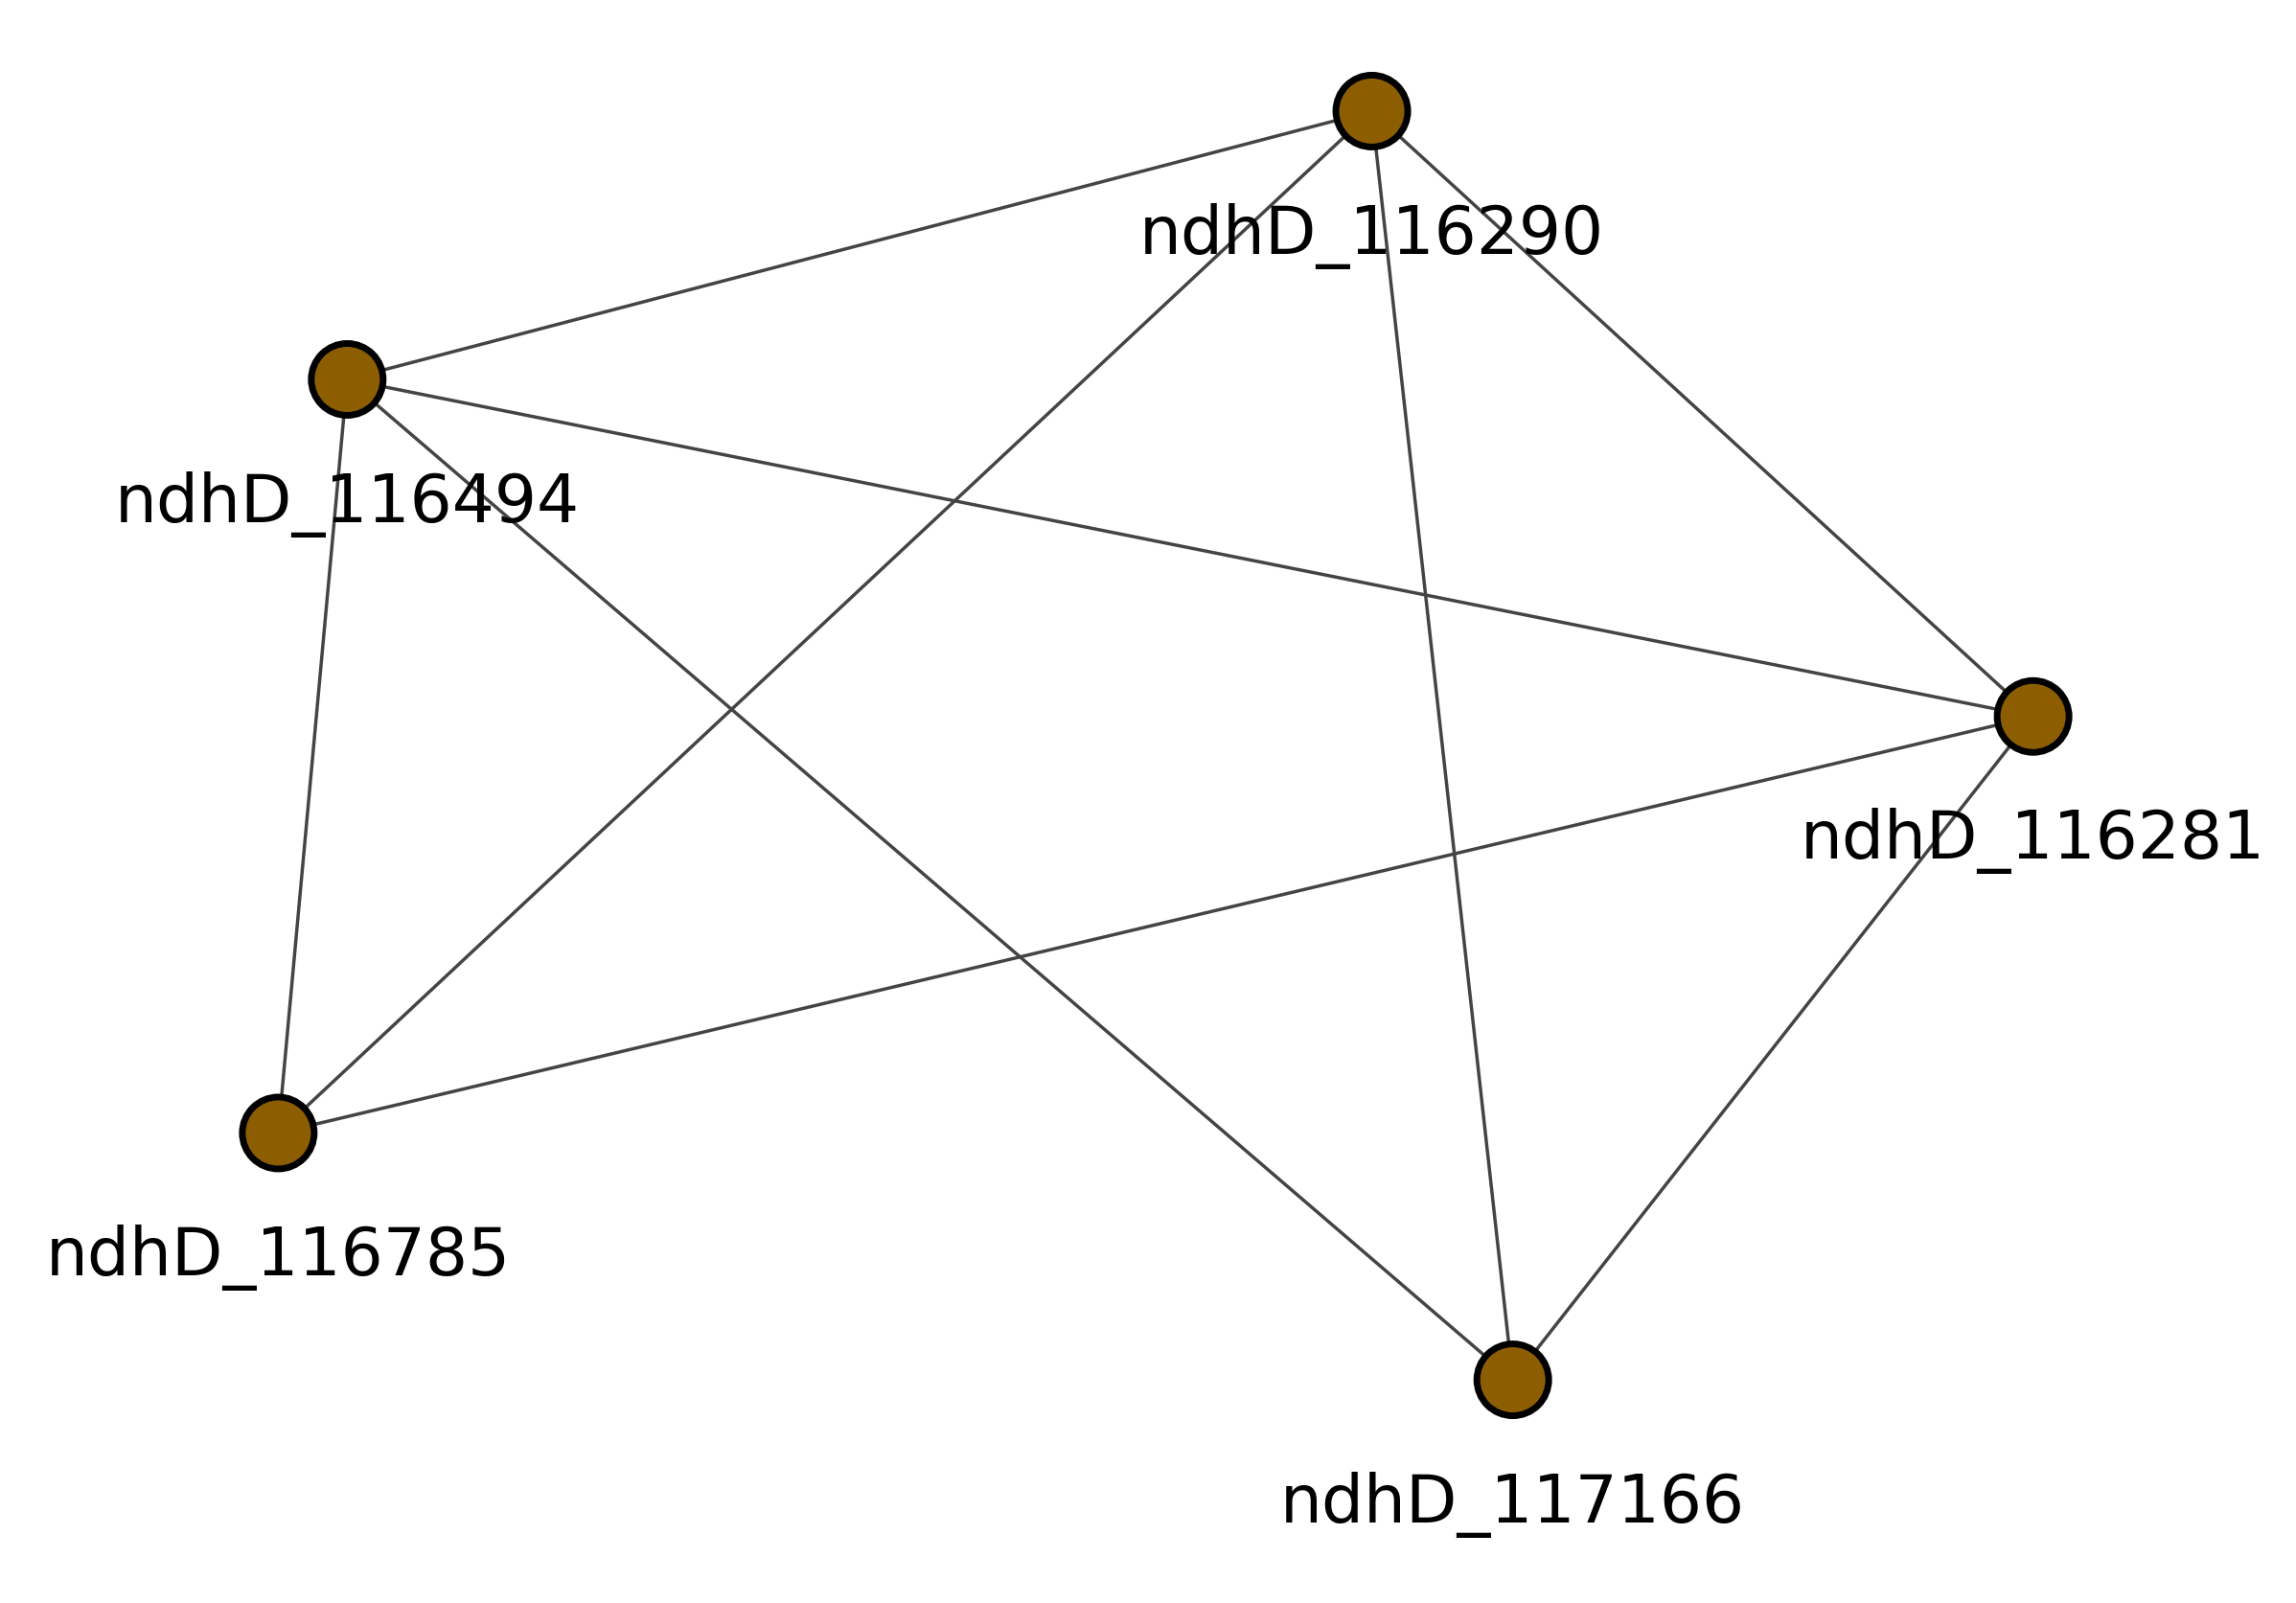
\includegraphics[width=3.125in,height=\textheight,keepaspectratio]{Figures Reference Graphs/depend_ndhD_Fig5.png}

}

\subcaption{\label{fig-ndhD-analysis-a}Dependencies network}

\end{minipage}%
%
\begin{minipage}{0.13\linewidth}
~\end{minipage}%
%
\begin{minipage}{0.43\linewidth}

\centering{

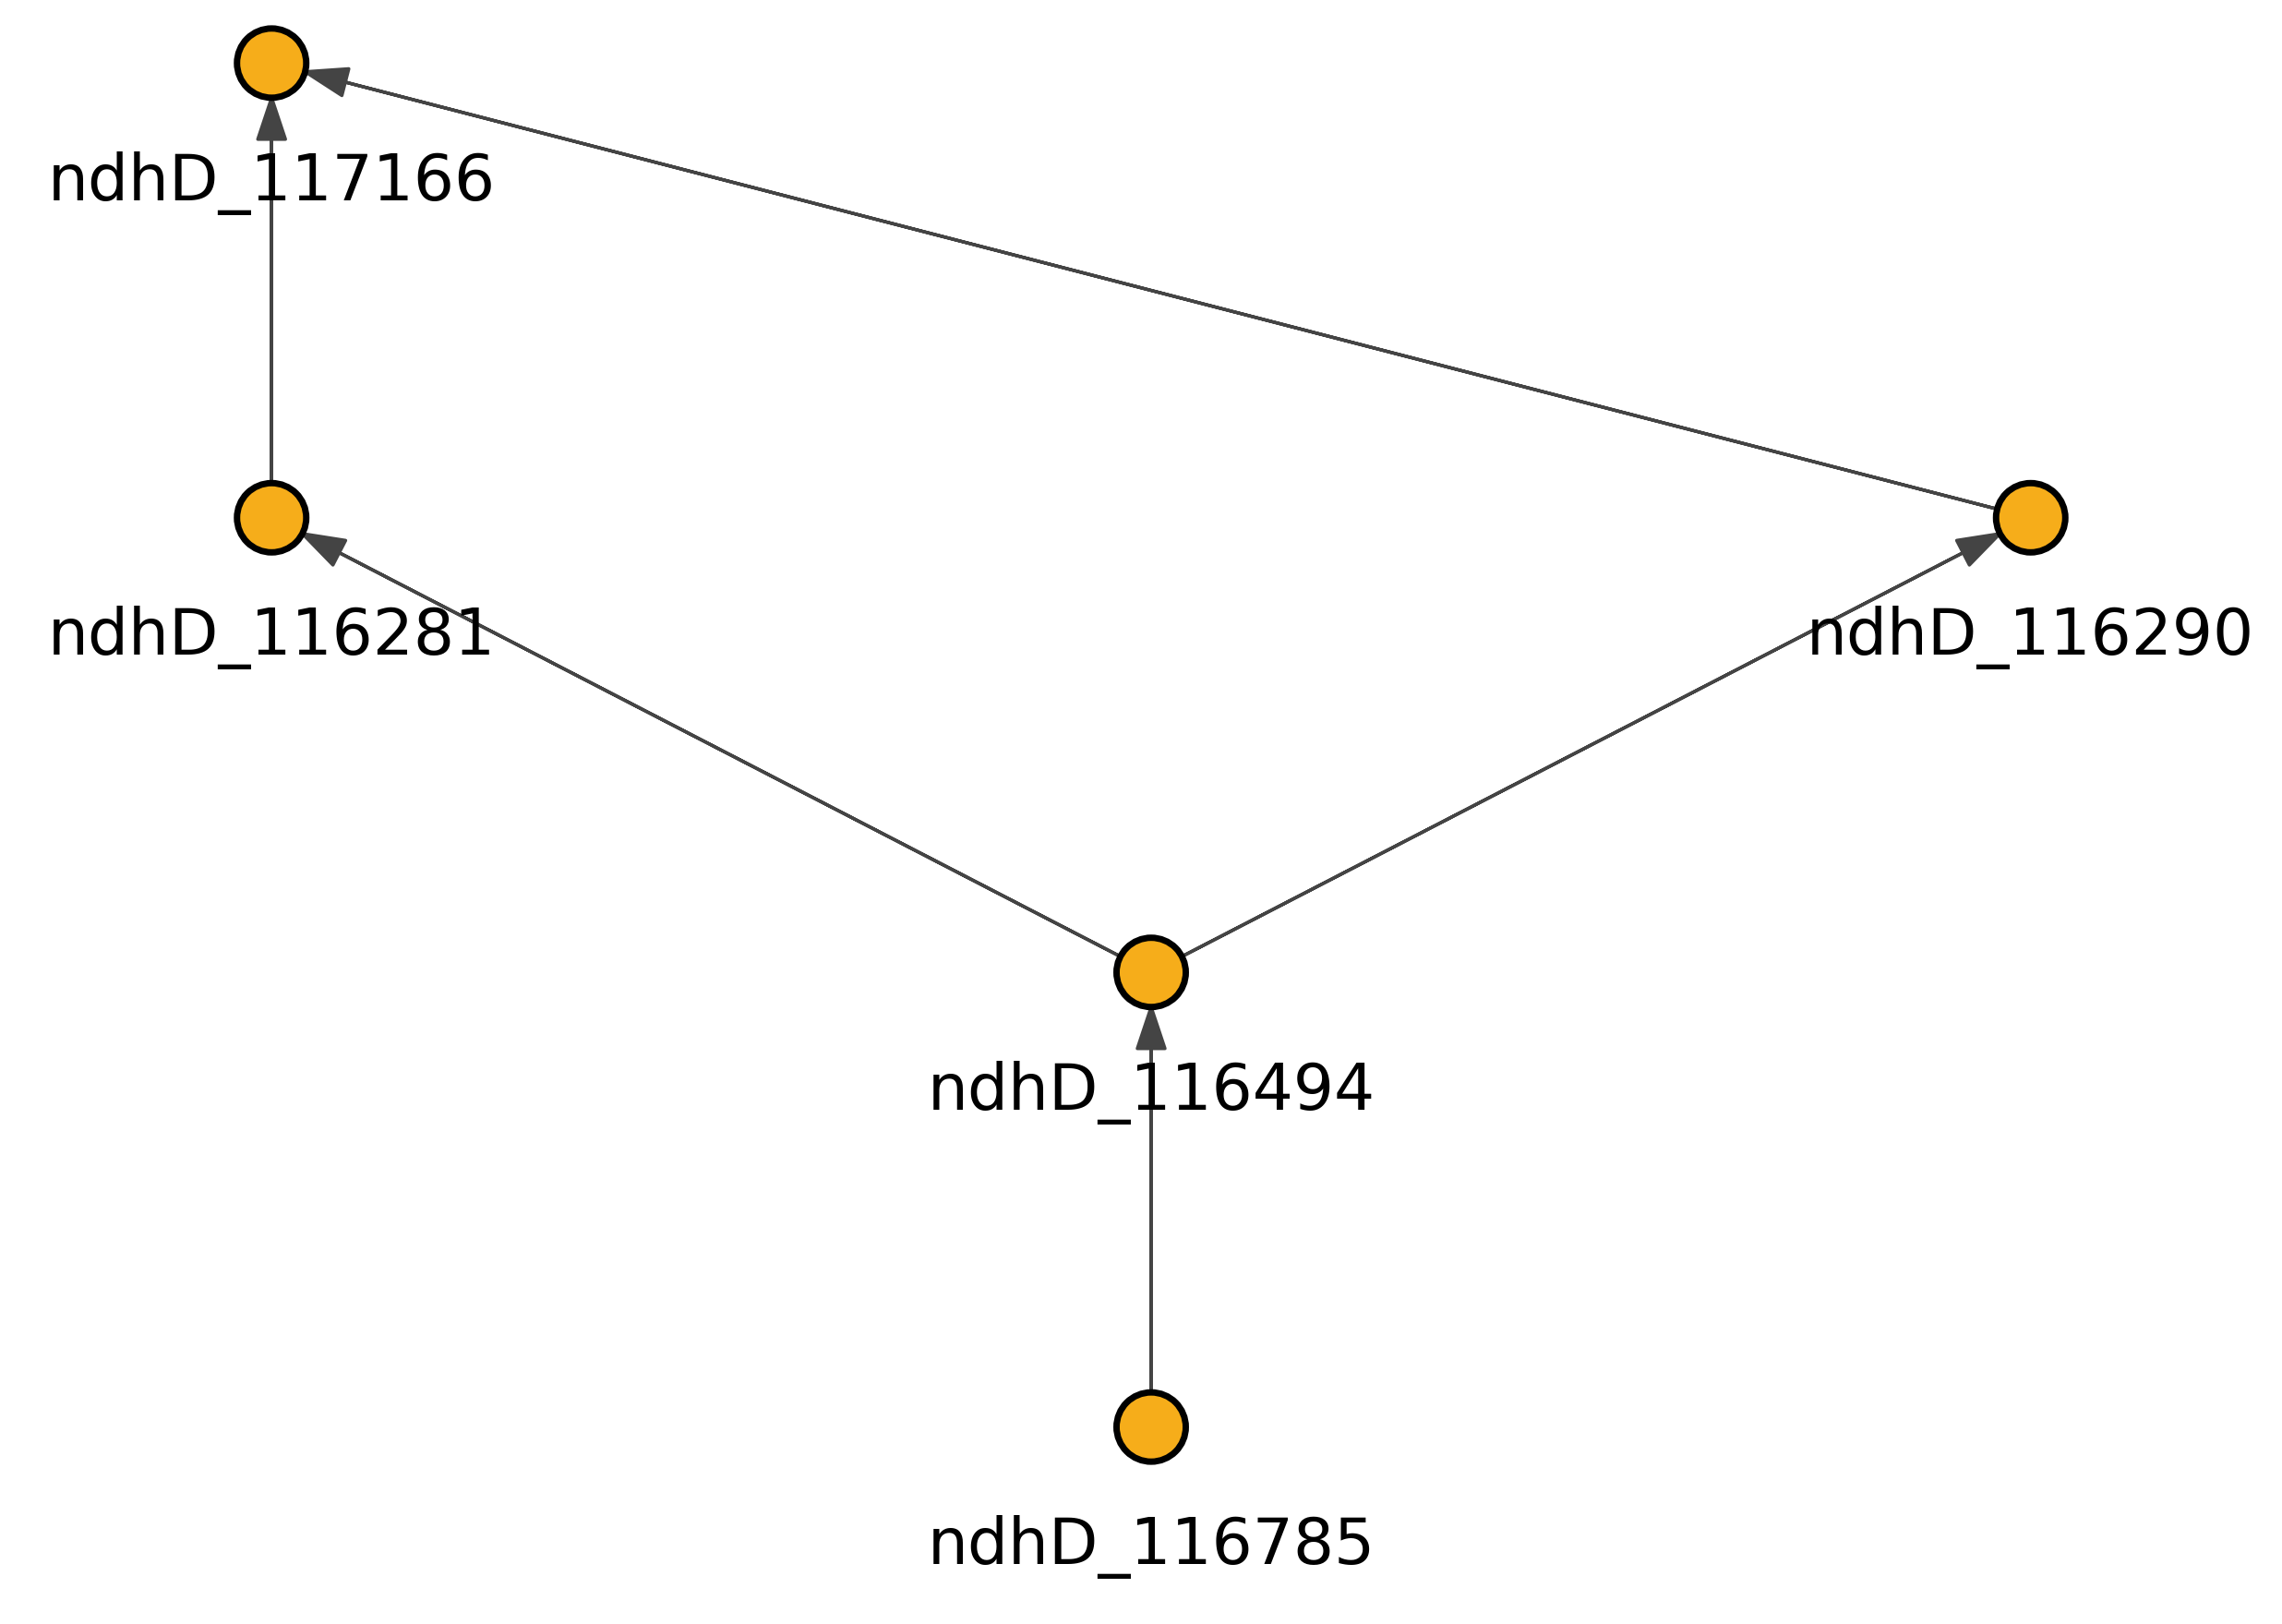
\includegraphics[width=3.125in,height=\textheight,keepaspectratio]{Figures Reference Graphs/chron_ndhD_Fig6.png}

}

\subcaption{\label{fig-ndhD-analysis-b}Reference maturation chronology}

\end{minipage}%

\caption{\label{fig-ndhD-analysis}Analysis of genetic regulation for
\emph{ndhD} from \citeproc{ref-Long_Reads_GuilcherEtAl}{{[}1{]}}: (a)
statistical dependencies between maturation events, and (b) resulting
directed acyclic graph representing the maturation timeline based on
frequency ordering.}

\end{figure}%

The previous conception is based on a determinist viewpoint, commonly
shared in the biological community: \emph{a maturation event strictly
depends on its predecessors: it is triggered by them and cannot occur
otherwise}. However, we know by now that the interactions between
different maturation events can be much more complex and intricate than
that (cf. \citeproc{ref-Heterologous_SchmitzEtAl}{{[}15{]}},
\citeproc{ref-LarchMito_MarechalEtAl}{{[}16{]}}.
\citeproc{ref-ChloroCP31A_TillichEtAl}{{[}17{]}},
\citeproc{ref-SiteSelective_KarcherBock}{{[}18{]}},
\citeproc{ref-CisElements_TakenakaNeuwirtBrennicke}{{[}19{]}}).

In this sense, our approach represents a paradigm shift based on the
following two objections to the deterministic postulate: \emph{an event
can have a strong causal effect even if it is rare} and
\emph{probabilistically some events can still happen without their
causal predecessors occurring}. Accordingly, a maturation event can
appear on the top of the maturation timeline even if it is hardly
observed alone (that is without other regulations).

A biological explanation for this phenomenon relates to the speed at
which events occur. Assume for example, that event \(A\) strongly or
rapidly promotes event \(B\), then \(B\) will quickly follow \(A\), so
\(A\) will rarely be observed alone. If we further assume that \(B\) can
occur (for some small probability) without \(A\) and \(B\) does not
promote \(A\), then \(B\) will often be observed without \(A\). In this
scenario \(A\) is the cause of \(B\), yet using the deterministic
viewpoint we would conclude otherwise.

Such circumstances can indeed be observed within the working dataset.
Namely, generating the frequency table of all five possible outcomes for
\emph{ndhD}, one can find instances of this phenomenon. Specifically,
Table~\ref{tbl-contigency_ed40_ed41} shows the contingency matrix for
the pair of maturation events located at the genomic sites 116494 and
116785. Let \(A:= \text{ndhD\_116494}\) and \(B:= \text{ndhD\_116785}\).
We observe that ndhD\_116494 appears much less frequently alone than
ndhD\_116785. According to the deterministic postulate, this would
suggest an arrow
\(\text{ndhD\_116785}\longrightarrow \text{ndhD\_116494}\), as shown in
Figure~\ref{fig-ndhD-analysis-b}. However, the causal Hill-Climbing
model (HC-model, \citeproc{ref-TeyssierKoller2005}{{[}20{]}}), for
example, proposes the reverse direction,
\(\text{ndhD\_116494}\longrightarrow \text{ndhD\_116785}\), as seen in
Figure~\ref{fig-causal_HCmodel_chron_ndhD}\footnote{In fact, most of our
  causal models propose this arrow (see
  Figure~\ref{fig-cross_analysis_ndhD}).}.

\begin{longtable}[]{@{}lll@{}}

\caption{\label{tbl-contigency_ed40_ed41}Contingency matrix for the pair
(ndhD\_116494, ndhD\_116785)}

\tabularnewline

\toprule\noalign{}
& ndhD\_116785 = 0 & ndhD\_116785 = 1 \\
\midrule\noalign{}
\endhead
\bottomrule\noalign{}
\endlastfoot
ndhD\_116494 = 0 & 82 & 144 \\
ndhD\_116494 = 1 & 39 & 304 \\

\end{longtable}

As we will see in Section~\ref{sec-chloro}, some of the proposed models
even yield a reversed chronology compared to the one proposed in
\citeproc{ref-Long_Reads_GuilcherEtAl}{{[}1{]}}. The causal HC-model
again serves as an example: the path
\(\text{ndhD\_116290}\longrightarrow\text{ndhD\_116494}\longrightarrow \text{ndhD\_116785}\)
from Figure~\ref{fig-causal_HCmodel_chron_ndhD} reflects a reversed
timeline relative to that proposed by the reference model in
Figure~\ref{fig-ndhD-analysis-b}.

Moreover, the frequency table allows the following counts:

\begin{itemize}
\tightlist
\item
  ndhD\_116290 appears \(8\) times alone.
\item
  ndhD\_116290 appears \(26\) times together with ndhD\_116494.
\item
  ndhD\_116290 appears \(262\) times together with both ndhD\_116494 and
  ndhD\_116785.
\end{itemize}

In other words, the event ndhD\_116290 strongly promotes ndhD\_116494,
so it is rarely observed alone (and ndhD\_116494 is often observed
without ndhD\_116290). Besides, we see an increasing number of
co-occurrences with the subsequent events of the proposed timeline.

\begin{figure}[H]

\centering{

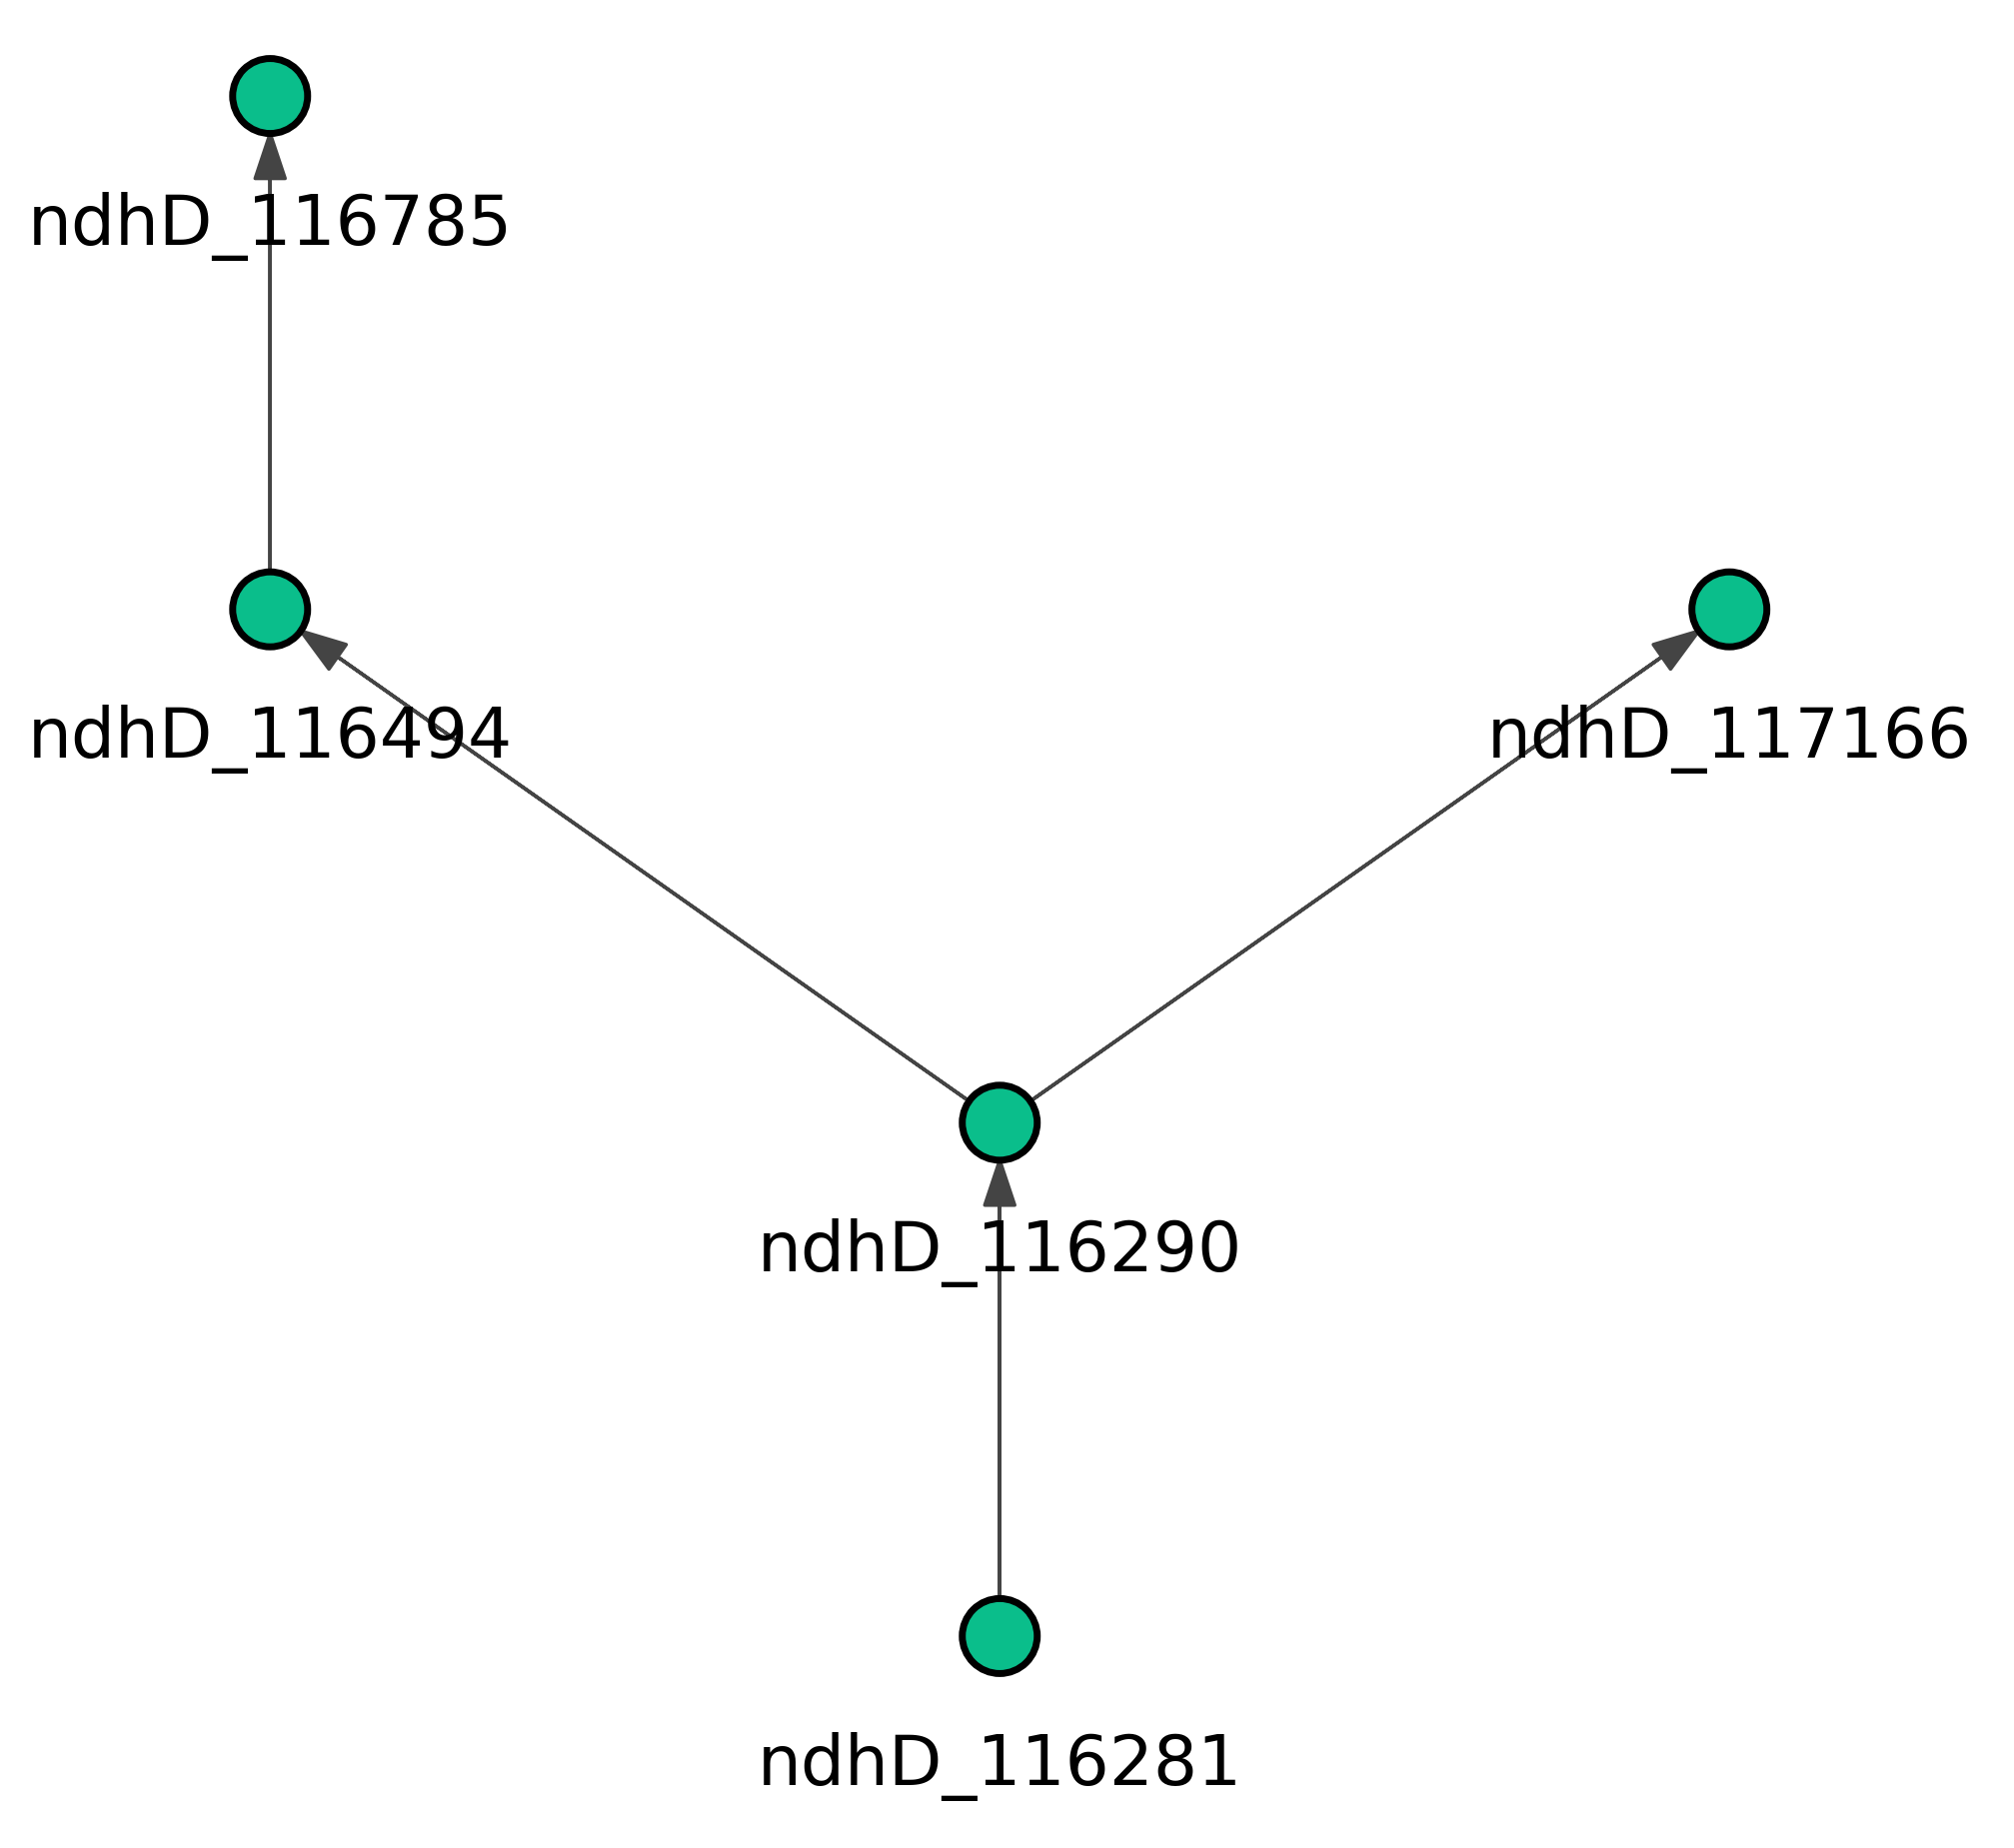
\includegraphics[width=3.125in,height=\textheight,keepaspectratio]{Figures Causal Chronology/chron_DAG_HC_ndhD.png}

}

\caption{\label{fig-causal_HCmodel_chron_ndhD}Causal HC-model for
maturation chronology for \emph{ndhD}}

\end{figure}%

More formally, the deterministic postulate relies on a connection
between the phenomenon \(\Big(\text{$A$ is the cause of $B$}\Big)\) and
the phenomenon
\(\Big(\text{$A$ is observed alone more often than $B$ alone}\Big)\).
However, from a probabilistic point of view, it is clear that the second
phenomenon does not allow to conclude any causal effect of \(A\) on
\(B\). Therefore, our paradigm shift consists in adopting a
probabilistic approach to the problem by directly computing
\(P(A\Rightarrow B)\). The mathematical framework for this is the causal
inference theory in terms of \emph{do-calculus} developped by J. Pearl
(cf. \citeproc{ref-CausalityBook_Pearl}{{[}13{]}},
\citeproc{ref-CausalityPaper_Pearl}{{[}21{]}}).

\begin{definition}[]\protect\hypertarget{def-CausalEffect}{}\label{def-CausalEffect}

We say that \(A\) has a causal effect on \(B\) if
\[P(B=1\ |\ \text{do($A=1$)}) > P(B=1\ |\ \text{do($A=0$)}).\]

We put \(P(A\Rightarrow B):= P(B=1\ |\ \text{do($A=1$)})\) and
\(P(\overline{A}\Rightarrow B):= P(B=1\ |\ \text{do($A=0$)})\).

\end{definition}

\begin{refremark}
It is apparent that there is a close relationship between
\emph{chronology} and \emph{causality}. Indeed, if \(B\) occurs before
\(A\), then \(A\) is definitely not a cause of \(B\). In other words,
causality entails a temporal order, hence a chronology.

\label{rem-chron_causality}

\end{refremark}

To conclude this section, we summarize the proposed pipeline within our
probabilistic framework, which is implemented and illustrated in
Section~\ref{sec-chloro}.

\begin{enumerate}
\def\labelenumi{\arabic{enumi}.}
\tightlist
\item
  \textbf{Causal discovery}. The first step is to infer a Directed
  Acyclic Graph (DAG) directly from the working dataset. We apply
  several well‑known methods: Hill Climbing (HC,
  \citeproc{ref-TeyssierKoller2005}{{[}20{]}}), Peter‑Clark (PC,
  \citeproc{ref-spirtes1993causation}{{[}22{]}}), LiNGAM
  \citeproc{ref-shimizu2006linear}{{[}23{]}}; and more recent continuous
  optimization variants such as NOTEARS
  \citeproc{ref-DagsNotears}{{[}14{]}}. This step involves both
  unconditional (statistical) dependence tests and conditional
  dependence tests, in order to establish directed edges between pairs
  of events in accordance with the observed data \footnote{This initial
    DAG contains a complex network of \emph{all} possible (directed)
    interdependencies between different events.}.
\end{enumerate}

\begin{enumerate}
\def\labelenumi{\arabic{enumi}.}
\setcounter{enumi}{1}
\item
  \textbf{Causal inference}. The first step yields a directed edge
  between two events, say \(A\rightarrow B\). This suggests that \(A\)
  is a potential cause of \(B\), though it may nevertheless happen that
  \(B\) occurs without \(A\). To decide whether \(A\) is an actual cause
  of \(B\), we perform a causal inference analysis: isolating the causal
  effect; identifying and adjusting for confounders; and, when possible,
  designing interventions or applying graphical criteria such as the
  \emph{backdoor criterion} to ensure that any spurious associations are
  removed.
\item
  \textbf{Chronology representation}. Finally, we construct the
  \emph{maximal causality path} based on the previous analysis. More
  precisely, among all causal effects, we retain only those with the
  highest impact, respecting the topological order of the initial DAG
  obtained in the first step. By the end of this procedure one obtains a
  tree (as a sub-DAG of the discovered DAG in the first step)
  representing the chronology between the maturation events\footnote{This
    tree reflects, by construction, the \emph{relevant} (directed)
    interdependence network between different events. In this sense, it
    represents the \emph{actual} causal structure underlying the initial
    DAG according to the \emph{causal minimality principle} (cf.
    \citeproc{ref-CausalityBook_Pearl}{{[}13{]}}).}.
\end{enumerate}

\section{Inferring Causal Maturation Timelines in Arabidopsis thaliana
via Bayesian Gene‑Regulation Models}\label{sec-chloro}

In this section, we apply the full causal inference pipeline described
earlier to the post-transcriptional maturation of two chloroplast genes
in \emph{Arabidopsis thaliana}: \textbf{\emph{ndhB}} and
\textbf{\emph{ndhD}}. These genes provide an ideal testing ground for
our methodology: they involve multiple sequential maturation
events---such as splicing and editing---captured in binary form from
full-length transcriptomic nanopore reads, and exhibit block-structured
missing data. Our goal is to infer robust and interpretable causal
chronologies of these events, going beyond mere co-occurrence or
frequency-based assumptions. Starting from imputed datasets, we learn
causal structures using HC, PC, LiNGAM, and NOTEARS, estimate causal
effects using do-calculus, and construct timeline DAGs that reflect
high-impact, directed causal relationships between maturation events.
The NOTEARS algorithm was adapted via a two-level stability selection
strategy to enhance robustness in the discovery of causal structures;
see Appendix Section~\ref{sec-notears} for details.

\subsection{Imputation through Bayesian network
discovery}\label{sec-imputation}

An important limitation of the datasets used to study gene regulation in
\emph{Arabidopsis thaliana} is the significant presence of missing
values. The distribution of these missing entries makes it impractical
to restrict the dataset to fully observed rows, as this would
drastically reduce the number of usable observations. This issue also
affects the first step of our pipeline--\textbf{\emph{Causal
discovery}}--. As a result, we must perform imputation jointly with the
learning of the corresponding Bayesian network.

To handle the full dataset, our strategy for missing data involves two
stages of imputation: 1. \textbf{\emph{Initial imputation}}, and 2.
\textbf{\emph{Graphical model imputation}}. Implementation details and
configuration settings are available in a
\href{https://github.com/cambroise/chloroDAG}{GitHub repository}.

\begin{enumerate}
\def\labelenumi{\arabic{enumi}.}
\item
  \textbf{Initial imputation}. First, we perform a preliminary imputaton
  of missing values in order to have a complete dataset as a starting
  point for learning the Bayesian Network (via the selected causal
  discovery algorithm). Technically, the initial imputation is carried
  out using the \texttt{IterativeImputer} class from the
  \texttt{scikit-learn} Python library (cf.
  \citeproc{ref-scikit-learnLibrary}{{[}24{]}}). This method models each
  feature with missing values as a function of other features, using
  those estimates for imputation in a round-robin fashion. At each step,
  one feature (i.e.~column) is treated as the target and the others as
  predictors.
\item
  \textbf{Graphical model imputation}. Next, we apply an
  \emph{Expectation-Maximization} (EM) algorithm to jointly refine the
  imputed values and the Bayesian Network. The EM algorithm alternates
  between two steps:

  \begin{itemize}
  \tightlist
  \item
    \textbf{E-step (Expectation):} Missing values are imputed using the
    current Bayesian Network. For each missing value:

    \begin{itemize}
    \tightlist
    \item
      The parents of the variable in the current DAG are identified.
    \item
      The corresponding Conditional Probability Distribution (CPD) is
      used to compute the most likely value for the missing entry, given
      its parents' values.
    \item
      The dataset is updated by replacing the missing value with this
      most probable estimate.
    \end{itemize}
  \item
    \textbf{M-step (Maximization):} A new Bayesian Network is learned
    from the updated dataset using the selected causal discovery
    algorithm (HC, PC, LiNGAM, or NOTEARS). This includes:

    \begin{itemize}
    \tightlist
    \item
      Re-learning the DAG structure from the completed data.
    \item
      Re-estimating the CPDs.
    \end{itemize}
  \end{itemize}
\end{enumerate}

These steps are repeated iteratively until convergence, defined as the
point where the proportion of changed directed edges between iterations
falls below 1\%.

\begin{refremark}
Numerical experiments with our gene regulation datasets have shown that
the choice of initial imputation method does not significantly affect
the resulting graphical model. For example, a simple \emph{mode}
imputation yields the same final network.

\label{rem-init_imp}

\end{refremark}

\begin{refremark}
The \textbf{\emph{Graphical model imputation}} method described above
converges rapidly. In fact, in our experiments, the network stabilizes
by the second iteration. One possible explanation for this efficiency
lies in the way missing values are updated: when a variable with missing
data is identified, the marginal probabilities required for its update
are computed using the values obtained from the initial imputation. That
is, even if some parent variables also had missing values originally,
they are treated as observed, based on the initial imputation.

A more principled approach would involve applying a \emph{Belief
Propagation} algorithm (cf.
\citeproc{ref-IntelligentSystemsBook_Pearl}{{[}25{]}},
\citeproc{ref-LoopyBP}{{[}26{]}}) in step (iv.c) to account for the
uncertainty in the imputed parent values. However, our experiments
indicate that this variant is significantly slower and does not lead to
any substantial refinement of the resulting Bayesian network. In
practice, the final graph is effectively the same as the one obtained
directly from the initial imputation, without applying any further
iterative refinement steps. One potential reason for this behavior is
that the \emph{Belief Propagation}-based version of the imputation
process imposes, by construction, rigid structural constraints on the
DAG, which in turn limits the ability of the EM algorithm to refine the
network structure.

\label{rem-Belief_Prop}

\end{refremark}

In our case study, we focus on datasets that describe the genetic
regulation of the \emph{ndhB} and \emph{ndhD} genes located in the
chloroplast of \emph{Arabidopsis thaliana}. We provide a brief
description of the datasets used and the distribution of missing
(\texttt{nan}) values.

Maturation events are modeled as binary random variables: \(1\) if
observed during post-transcriptional maturation, \(0\) otherwise. Errors
introduced by the nanopore sequencing technology used in
\citeproc{ref-Long_Reads_GuilcherEtAl}{{[}1{]}} are treated as
unobserved events and assigned a value of \(0\) during initial
pre-processing---an approach consistent with the binary encoding.

\subsubsection*{\texorpdfstring{\emph{ndhB}
dataset}{ndhB dataset}}\label{ndhb-dataset}

\begin{itemize}
\tightlist
\item
  \textbf{No.~observations}: \(1899\) including \(117\) fully observed.
\item
  \textbf{No.~maturation events}: \(12\) whose sites are \(94622\),
  \(94999\), \(95225\), \(95608\), \(95644\), \(95650\), \(96419\),
  \(96439\), \(96457\), \(96579\), \(96698\), \(97016\).
\item
  \textbf{Distribution of \texttt{nan} values}. Each observation
  contains a \emph{unique} block with consecutive reads, i.e.~there is
  no isolated reads in the genomic region between \texttt{nan} values.
  Figure~\ref{fig-ndhB_nan_distr} shows a visualisation of the
  distribution of the values of the \emph{ndhB} dataset before the
  imputation process described previously.
\end{itemize}

\begin{figure}[H]

\centering{

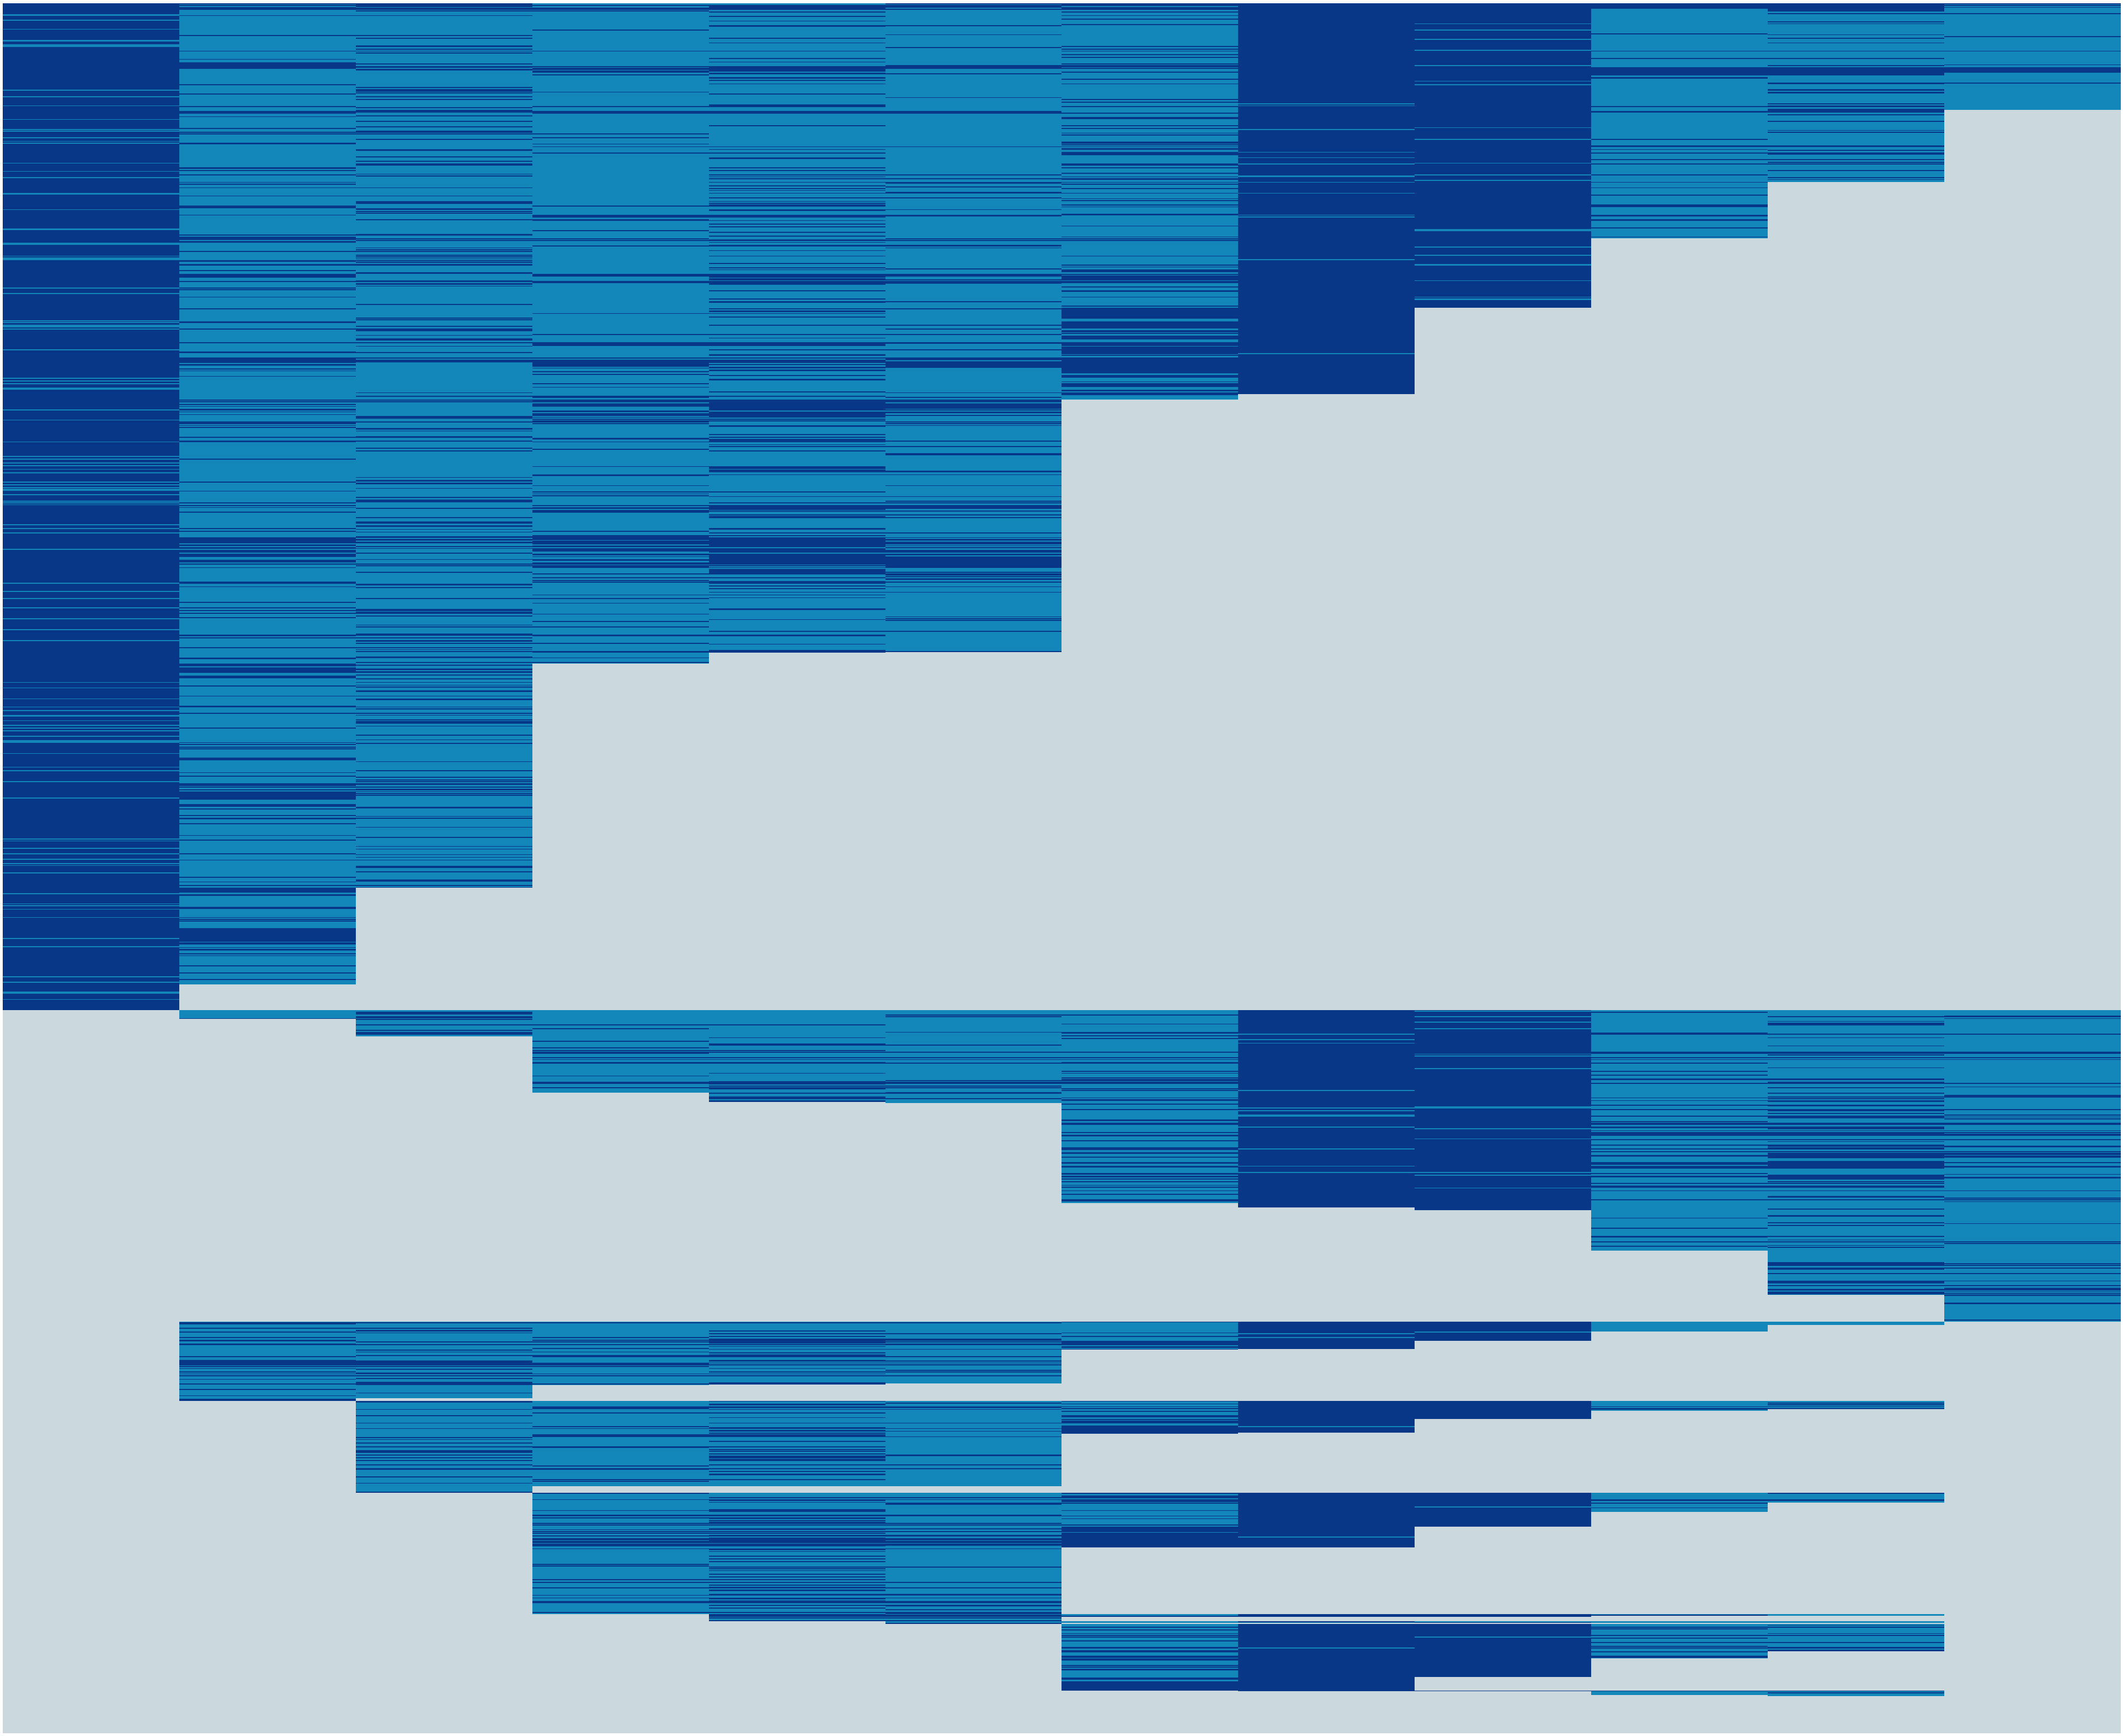
\includegraphics[width=0.4\linewidth,height=\textheight,keepaspectratio]{Figures NaN distributions/ndhB_visu_sorted.png}

}

\caption{\label{fig-ndhB_nan_distr}Distribution of values for
\emph{ndhB} before imputation: \(\color{MyDarkBlue}{\blacksquare}\)
\(=\) value \(0\), \(\color{MyBlue}{\blacksquare}\) \(=\) value \(1\),
\(\color{MySmokyBlue}{\blacksquare}\) \(=\) value \texttt{nan}}

\end{figure}%

\subsubsection*{\texorpdfstring{\emph{ndhD}
dataset}{ndhD dataset}}\label{ndhd-dataset}

\begin{itemize}
\tightlist
\item
  \textbf{No.~observations}: \(7752\) including \(930\) fully observed.
\item
  \textbf{No.~maturation events}: \(5\) whose sites are \(116281\),
  \(116290\), \(116494\), \(116785\), \(117166\).
\item
  \textbf{Distribution of \texttt{nan} values}. Each observation
  contains a \emph{unique} block with consecutive reads, i.e.~there is
  no isolated reads in the genomic region between \texttt{nan} values.
  Figure~\ref{fig-ndhD_nan_distr} shows a visualisation of the
  distribution of the values of the \emph{ndhD} dataset before the
  imputation process described previously.
\end{itemize}

\begin{figure}[H]

\centering{

\includegraphics[width=0.18\linewidth,height=\textheight,keepaspectratio]{Figures NaN distributions/ndhD_visu_sorted.png}

}

\caption{\label{fig-ndhD_nan_distr}Distribution of values for
\emph{ndhD} before imputation: \(\color{MyDarkBlue}{\blacksquare}\)
\(=\) value \(0\), \(\color{MyBlue}{\blacksquare}\) \(=\) value \(1\),
\(\color{MySmokyBlue}{\blacksquare}\) \(=\) value \texttt{nan}}

\end{figure}%

\subsection{Causal inference}\label{sec-quantitative-causality}

In this section, we detail the implementation of our probabilistic
approach applied to the \emph{ndhB} and \emph{ndhD} genes of the
chloroplast of \emph{Arabidopsis thaliana}.

The first step in our pipeline is \textbf{\emph{Causal discovery}}. The
graphs in Figure~\ref{fig-CD_ndhB} and Figure~\ref{fig-CD_ndhD}
represent the discovered DAGs from the working datasets (i.e.~after the
imputation process described in Section~\ref{sec-imputation}), obtained
using the HC, PC, LiNGAM, and NOTEARS algorithms. The HC and PC
algorithms are implemented via the \texttt{pgmpy} Python package (cf.
\citeproc{ref-pgmpyLibrary}{{[}27{]}}), while LiNGAM is implemented
using the \texttt{causal-learn} package (cf.
\citeproc{ref-CausalLearnLibrary}{{[}28{]}}). Implementation details and
configuration settings are available at our
\href{https://github.com/cambroise/chloroDAG}{GitHub repository}.

\begin{figure}[H]

\begin{minipage}{0.43\linewidth}

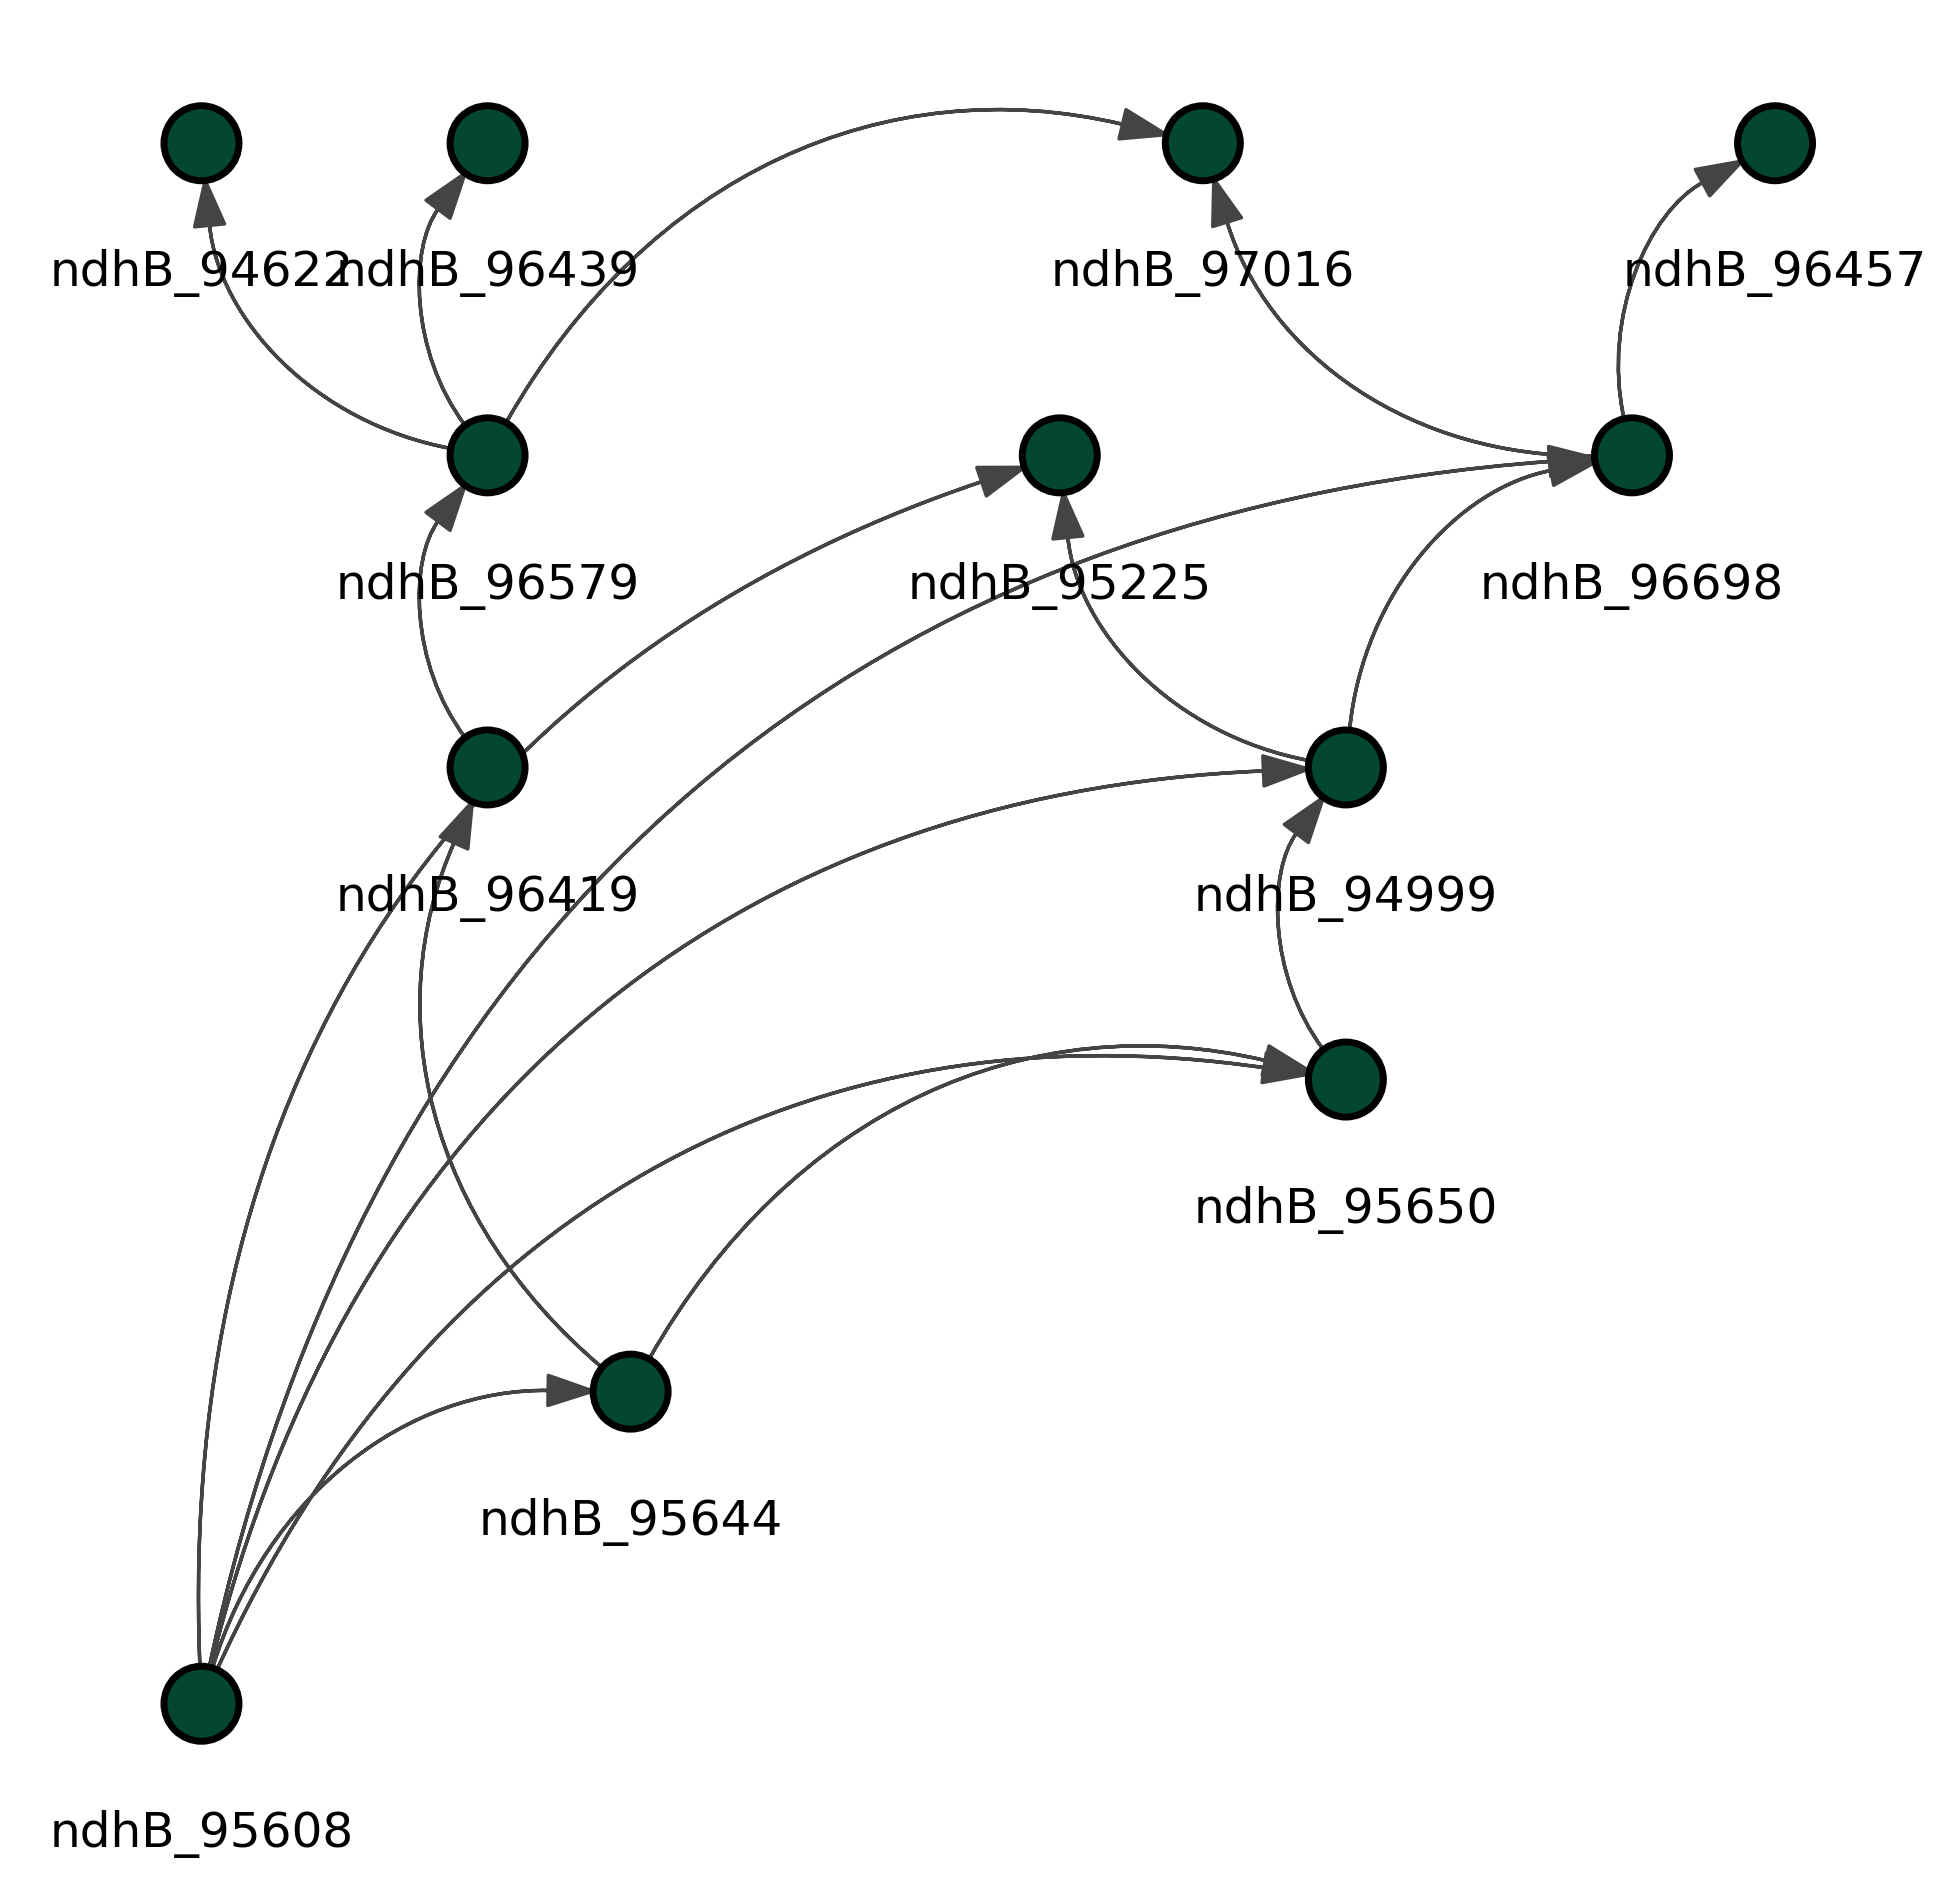
\includegraphics[width=3.125in,height=\textheight,keepaspectratio]{Figures Causal Discovery/DAG_HC_ndhB.png}

\subcaption{\label{}HC}
\end{minipage}%
%
\begin{minipage}{0.13\linewidth}
~\end{minipage}%
%
\begin{minipage}{0.43\linewidth}

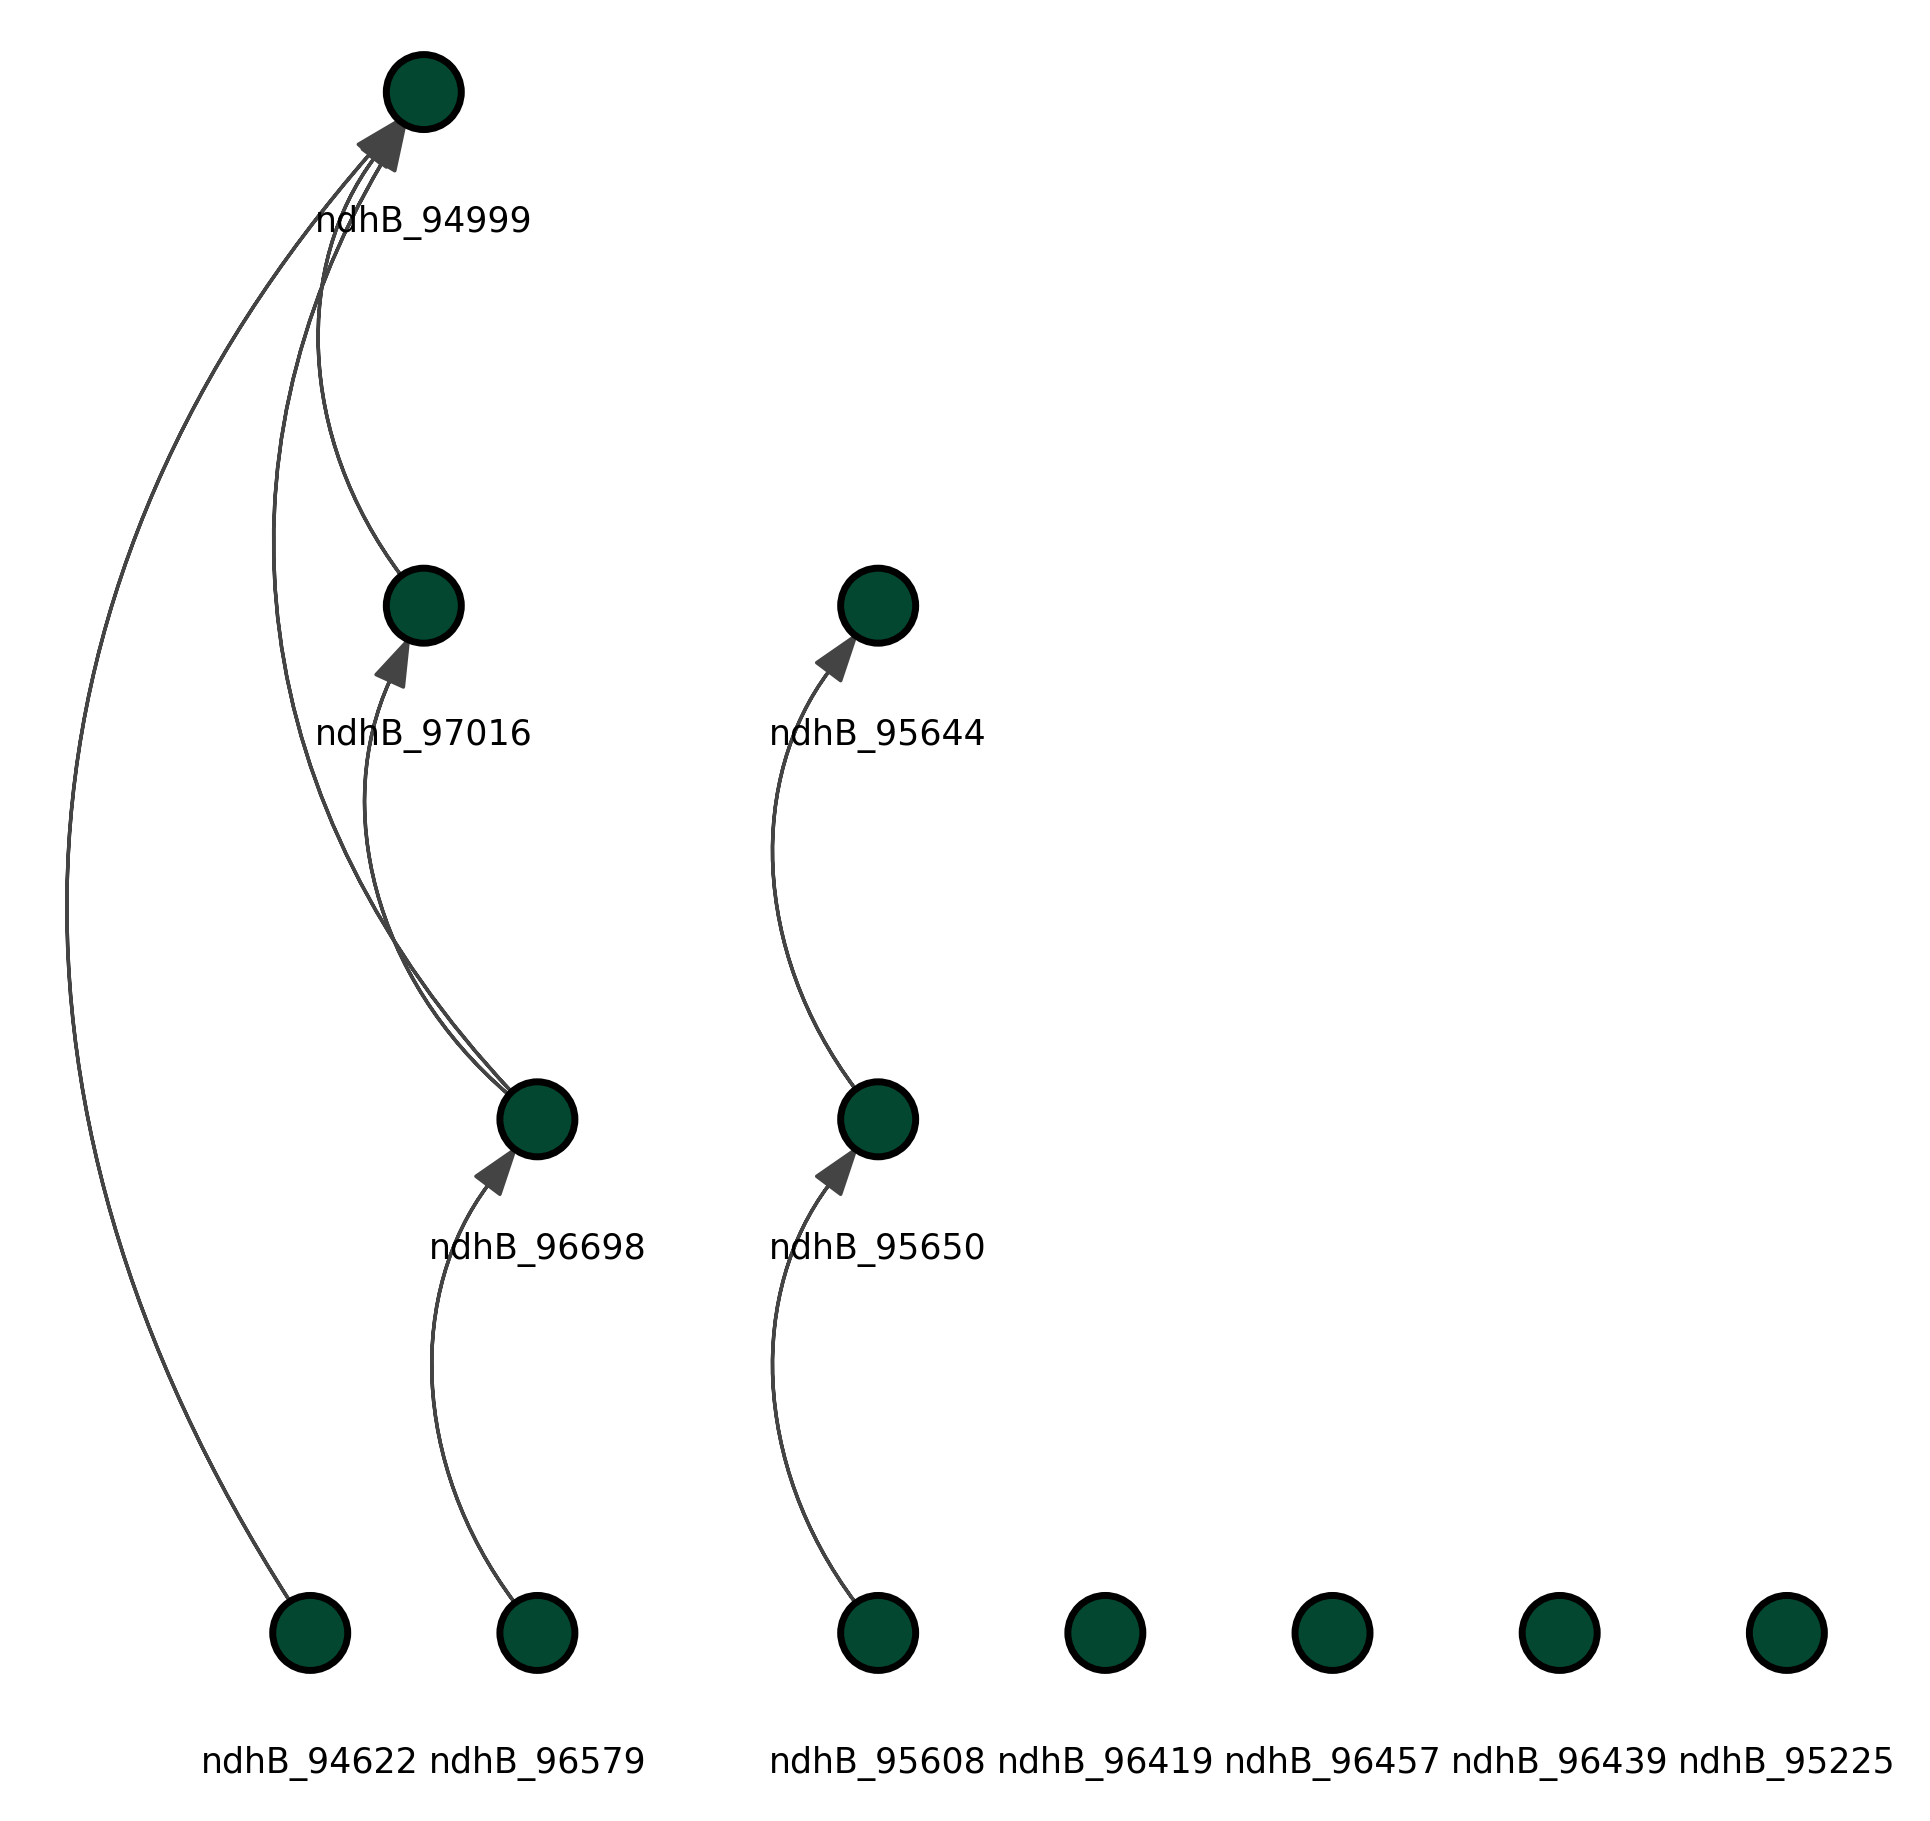
\includegraphics[width=3.64583in,height=\textheight,keepaspectratio]{Figures Causal Discovery/DAG_PC_ndhB.png}

\subcaption{\label{}PC}
\end{minipage}%
\newline
\begin{minipage}{0.43\linewidth}

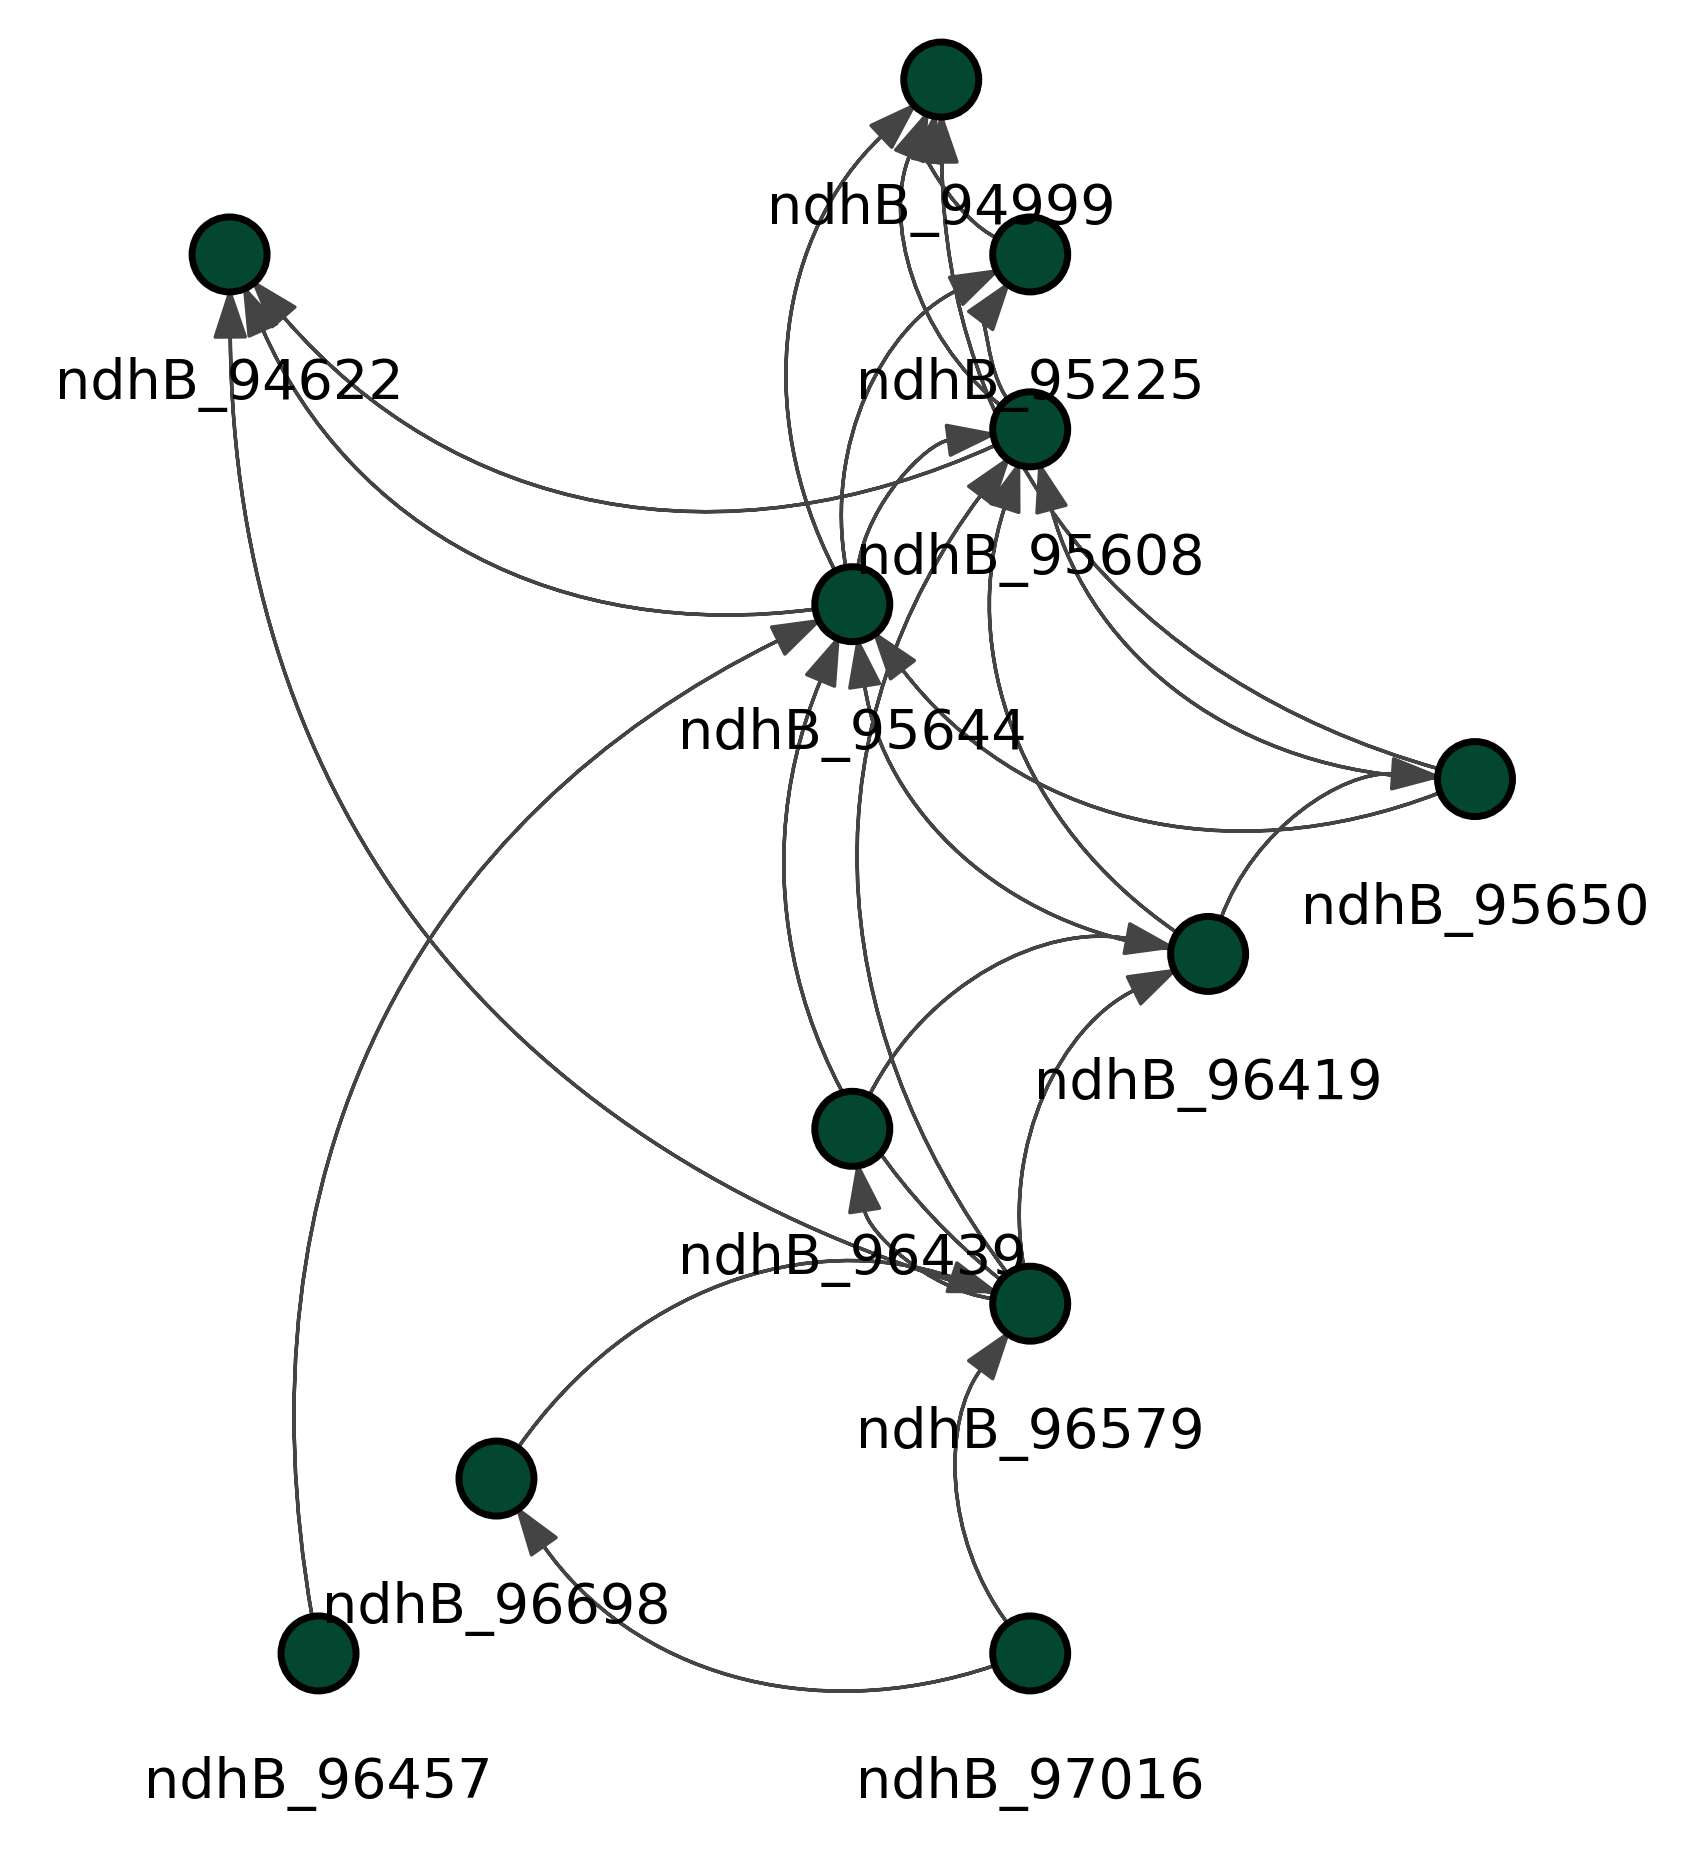
\includegraphics[width=3.125in,height=\textheight,keepaspectratio]{Figures Causal Discovery/DAG_LiNGAM_ndhB.png}

\subcaption{\label{}LiNGAM}
\end{minipage}%
%
\begin{minipage}{0.13\linewidth}
~\end{minipage}%
%
\begin{minipage}{0.43\linewidth}

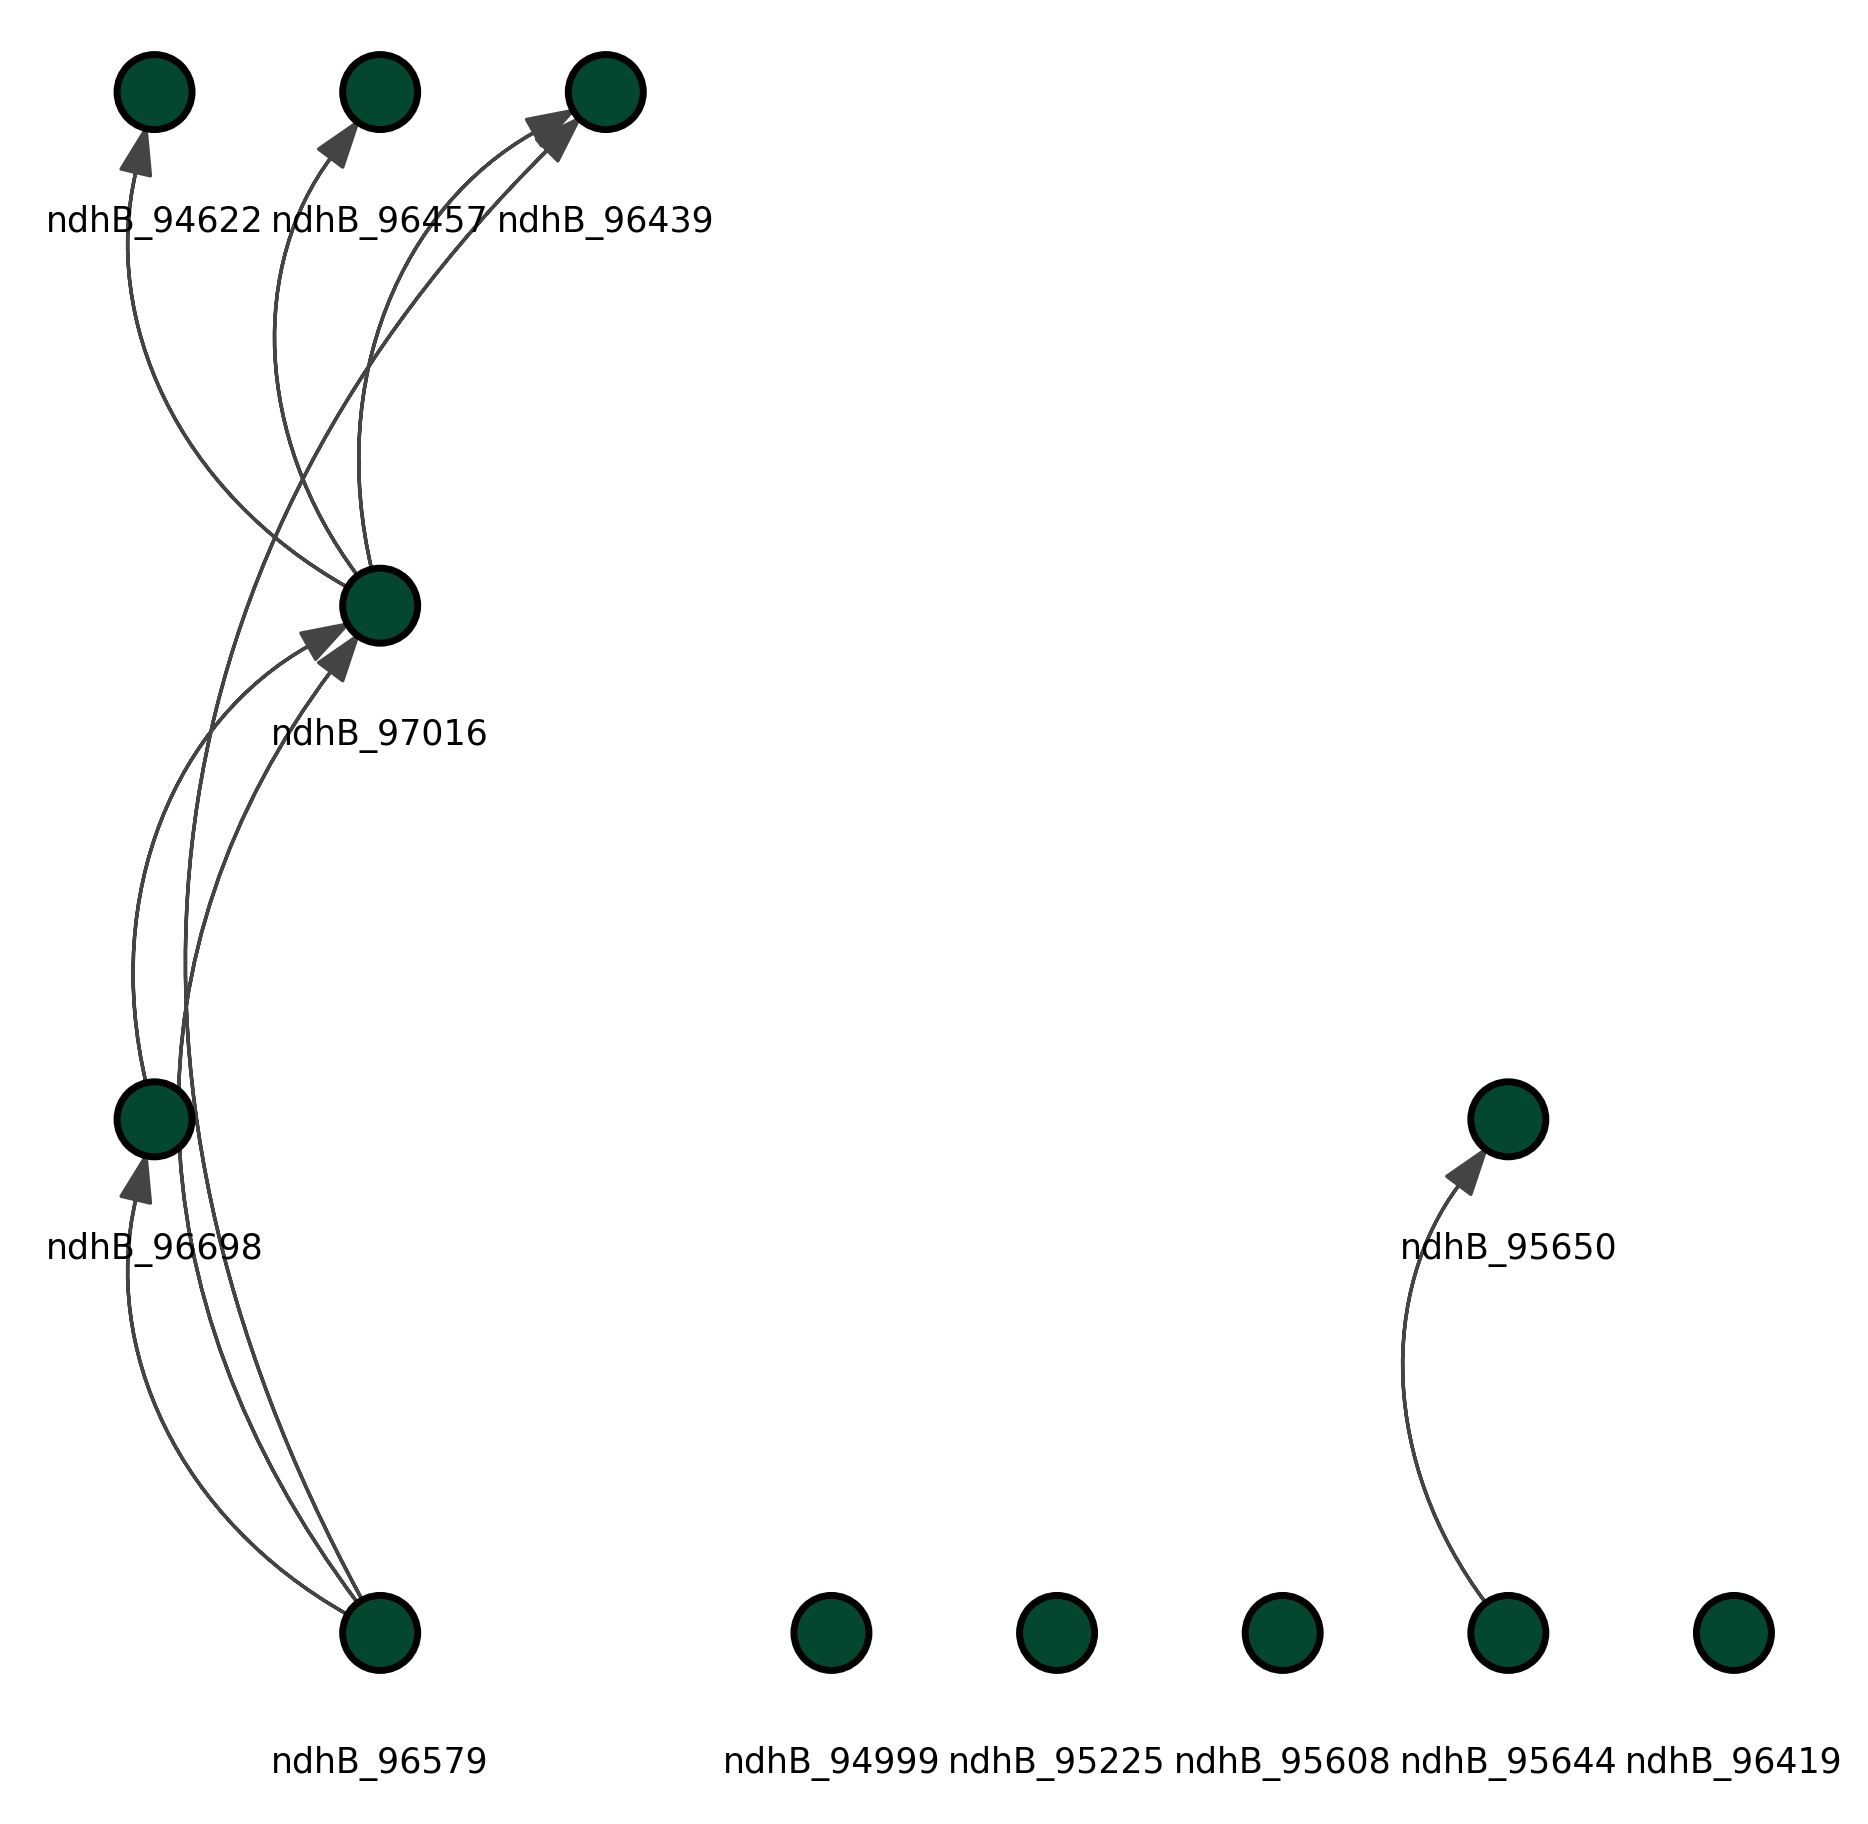
\includegraphics[width=3.64583in,height=\textheight,keepaspectratio]{Figures Causal Discovery/DAG_NOTEARS_ndhB.png}

\subcaption{\label{}NOTEARS}
\end{minipage}%

\caption{\label{fig-CD_ndhB}Causal Discovery for \emph{ndhB}}

\end{figure}%

\begin{figure}[H]

\begin{minipage}{0.43\linewidth}

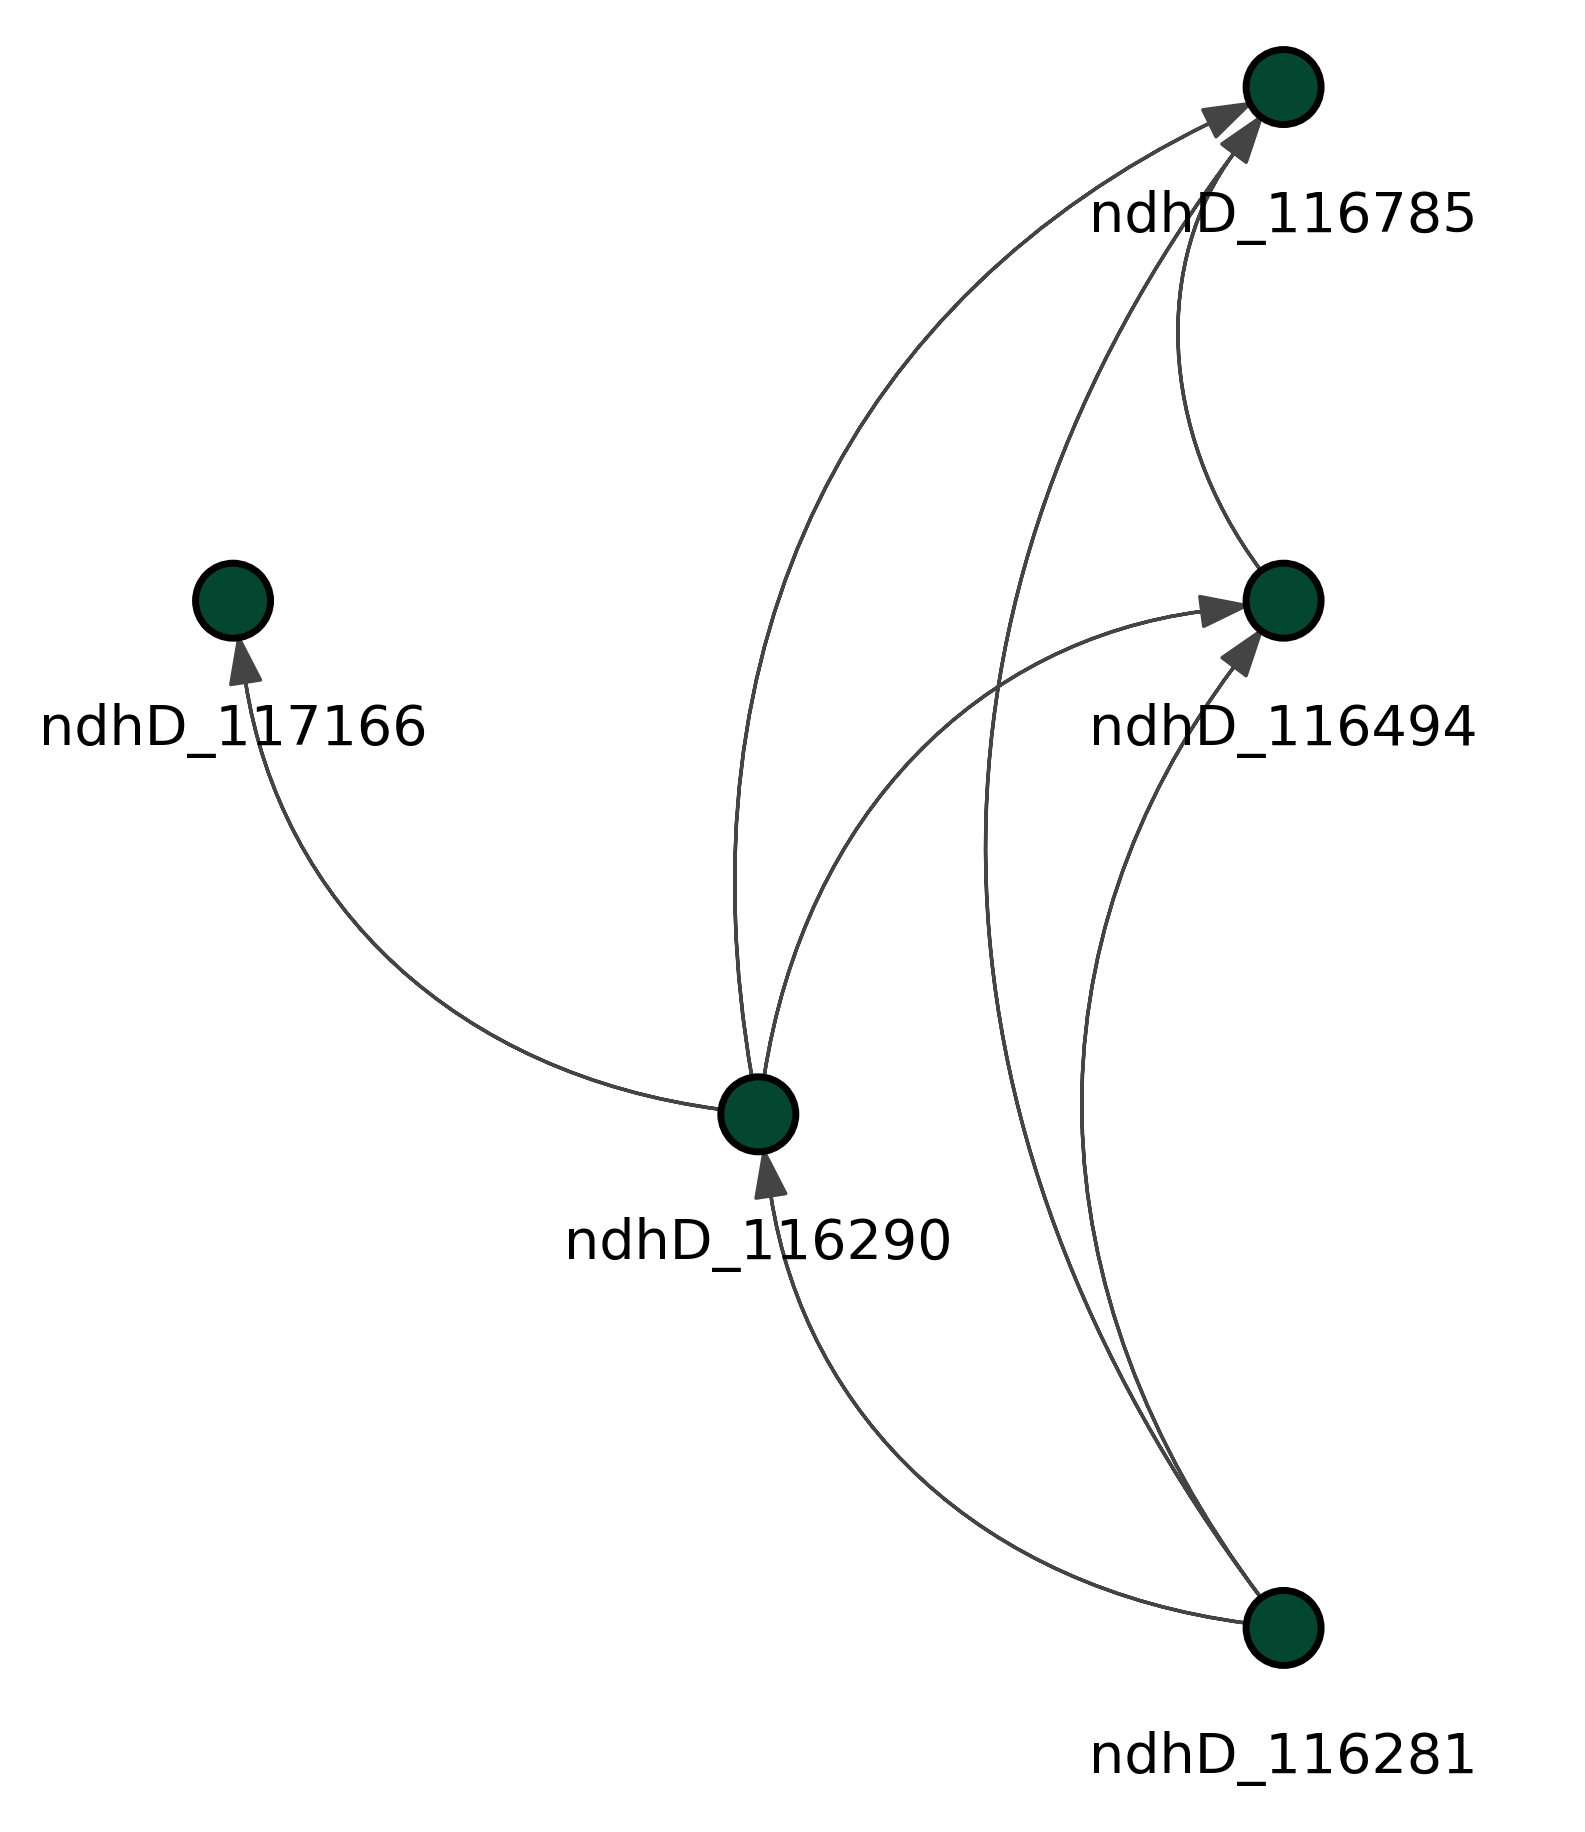
\includegraphics[width=3.125in,height=\textheight,keepaspectratio]{Figures Causal Discovery/DAG_HC_ndhD.png}

\subcaption{\label{}HC}
\end{minipage}%
%
\begin{minipage}{0.13\linewidth}
~\end{minipage}%
%
\begin{minipage}{0.43\linewidth}

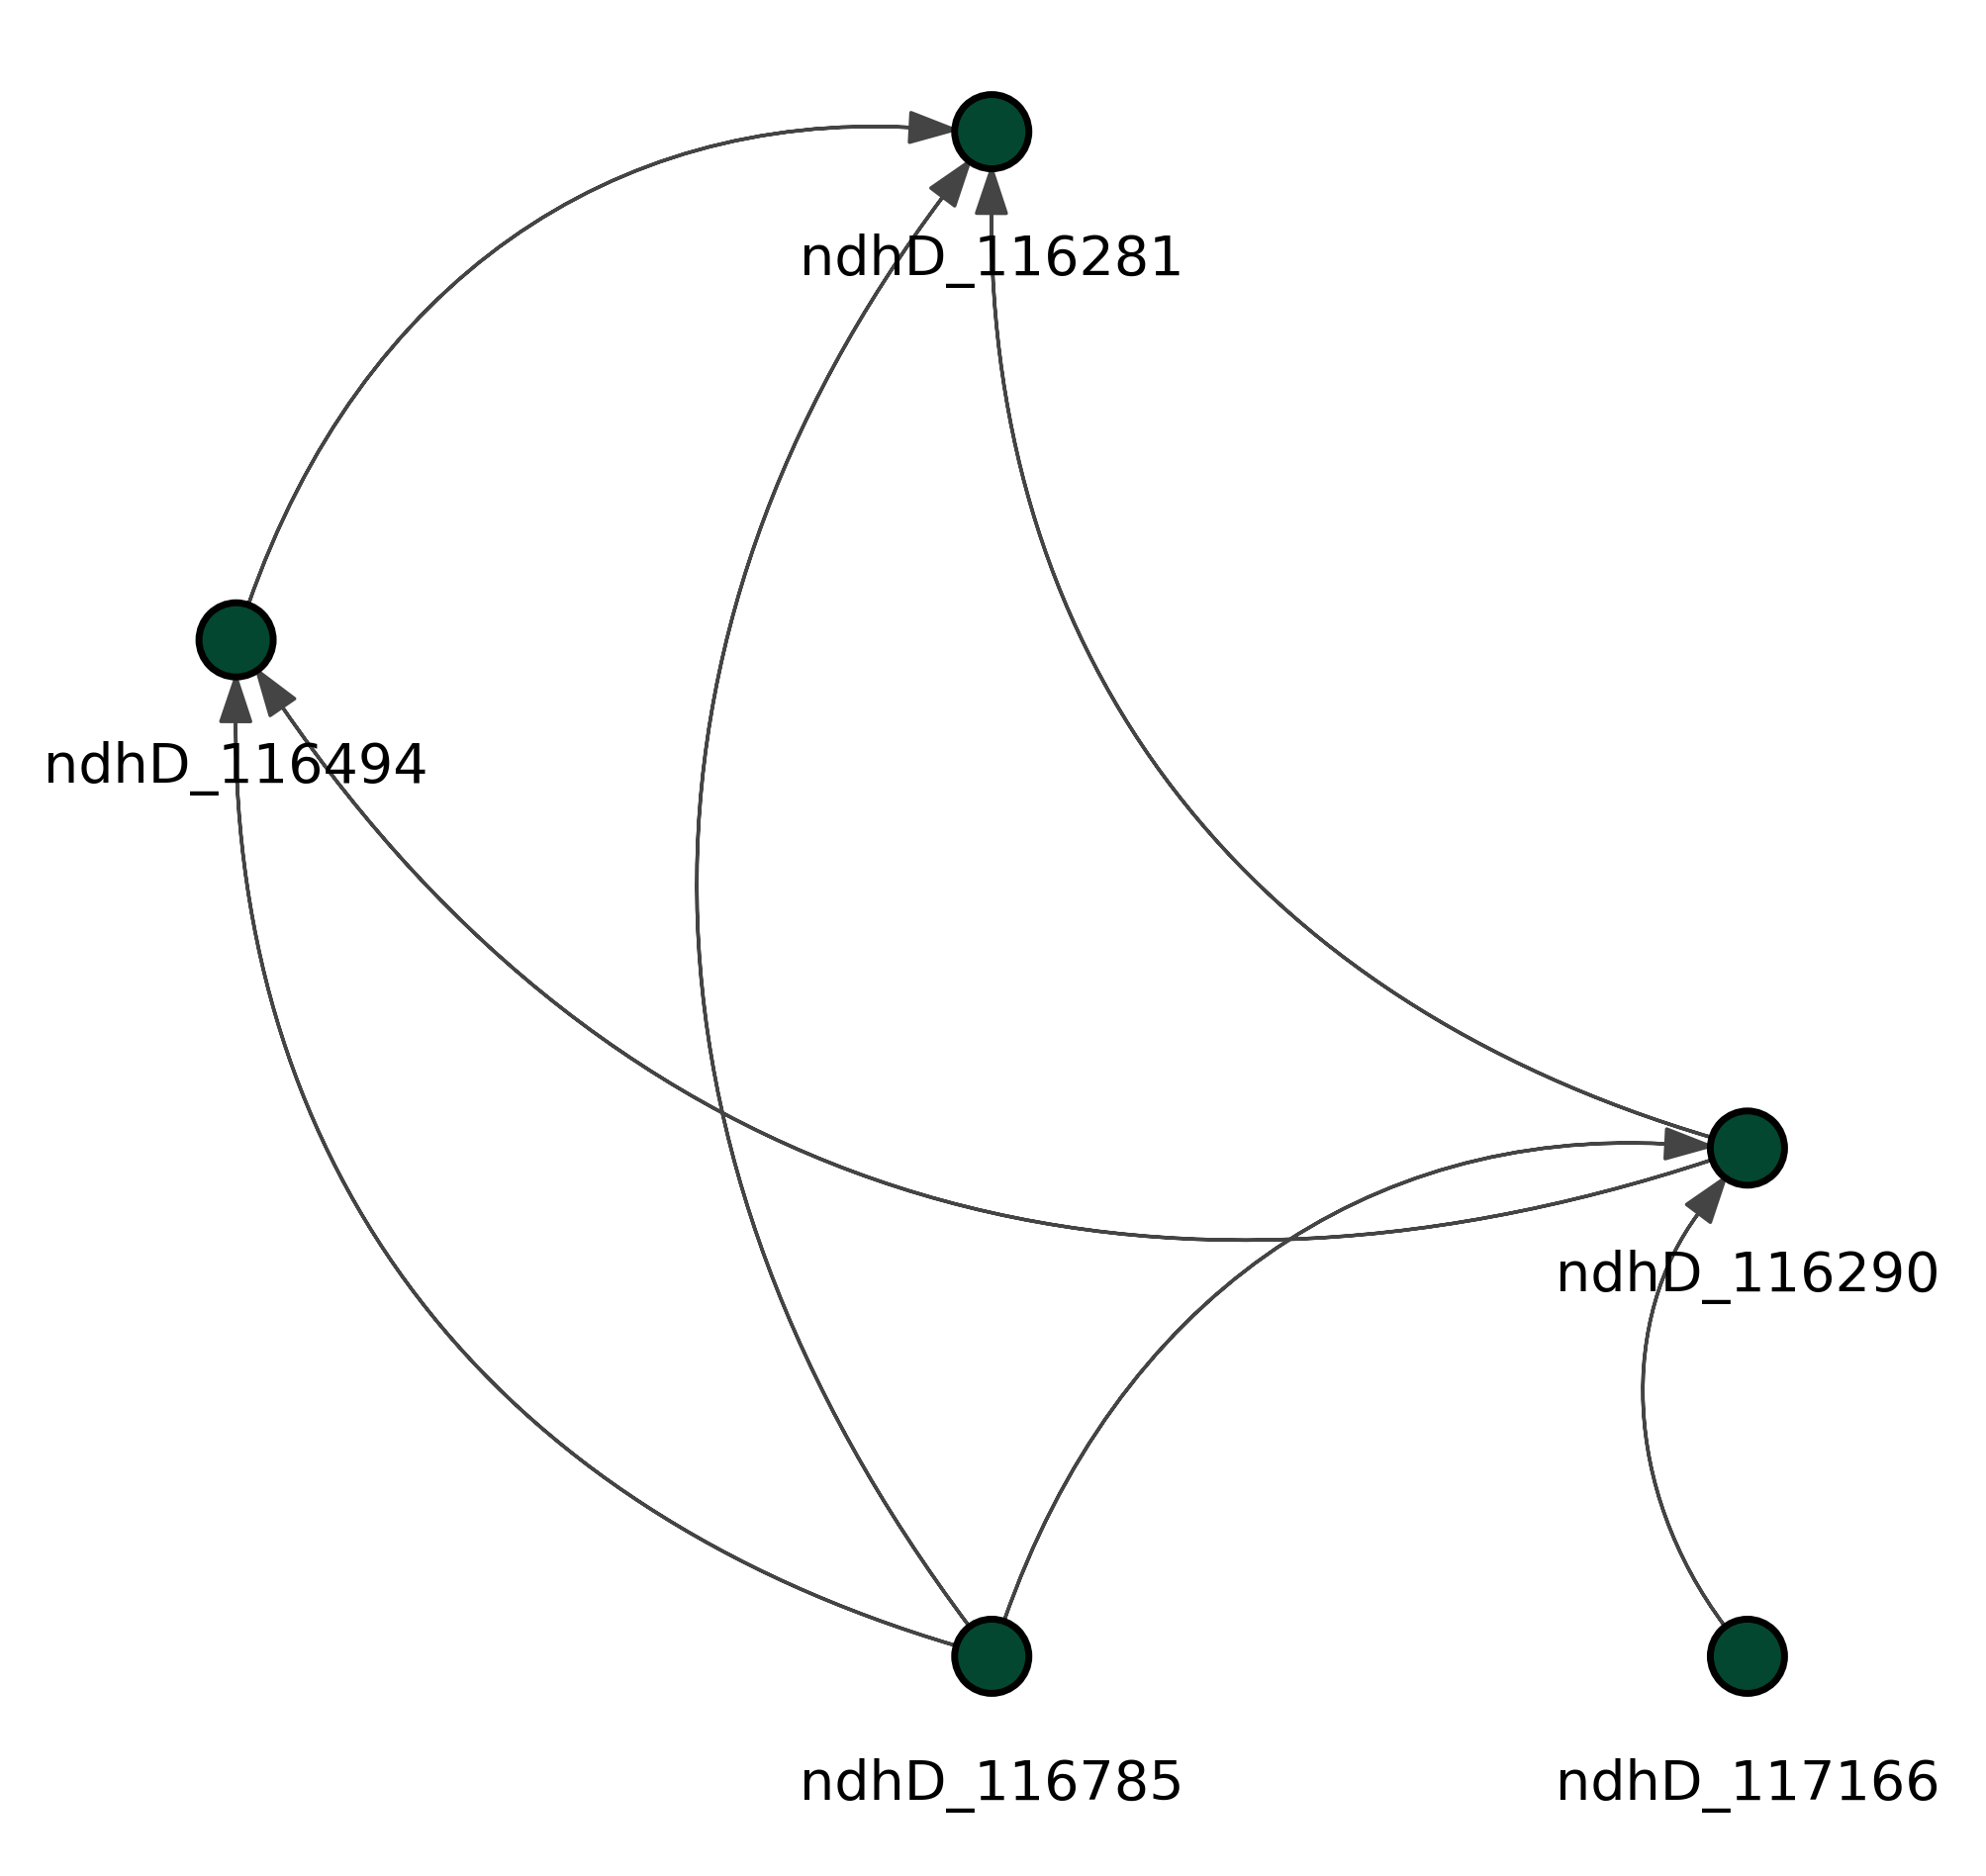
\includegraphics[width=3.64583in,height=\textheight,keepaspectratio]{Figures Causal Discovery/DAG_PC_ndhD.png}

\subcaption{\label{}PC}
\end{minipage}%
\newline
\begin{minipage}{0.43\linewidth}

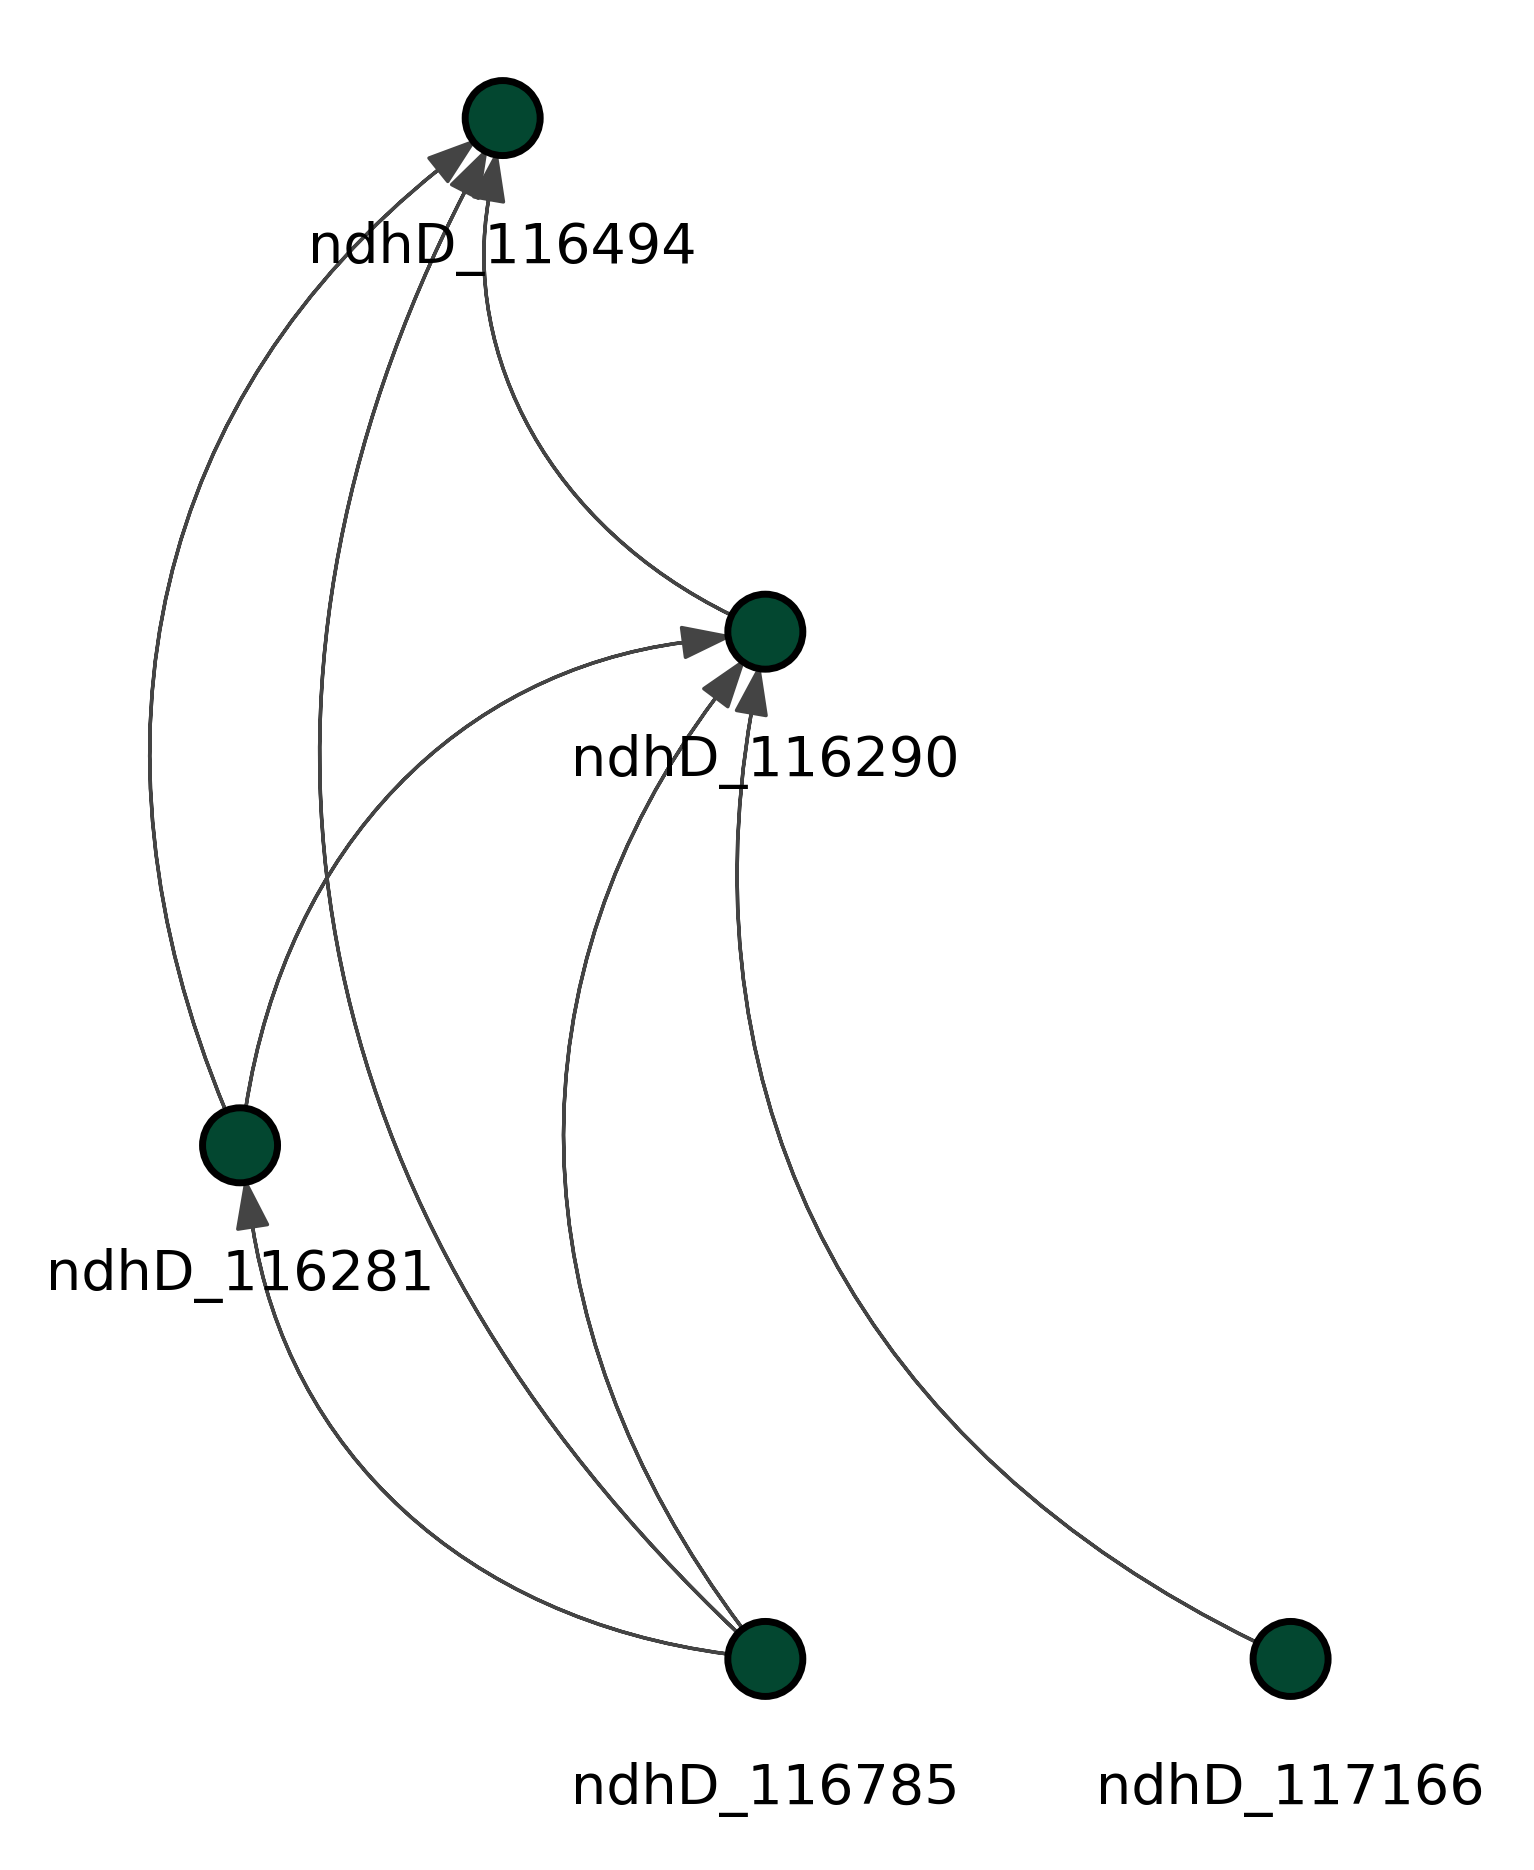
\includegraphics[width=3.125in,height=\textheight,keepaspectratio]{Figures Causal Discovery/DAG_LiNGAM_ndhD.png}

\subcaption{\label{}LiNGAM}
\end{minipage}%
%
\begin{minipage}{0.13\linewidth}
~\end{minipage}%
%
\begin{minipage}{0.43\linewidth}

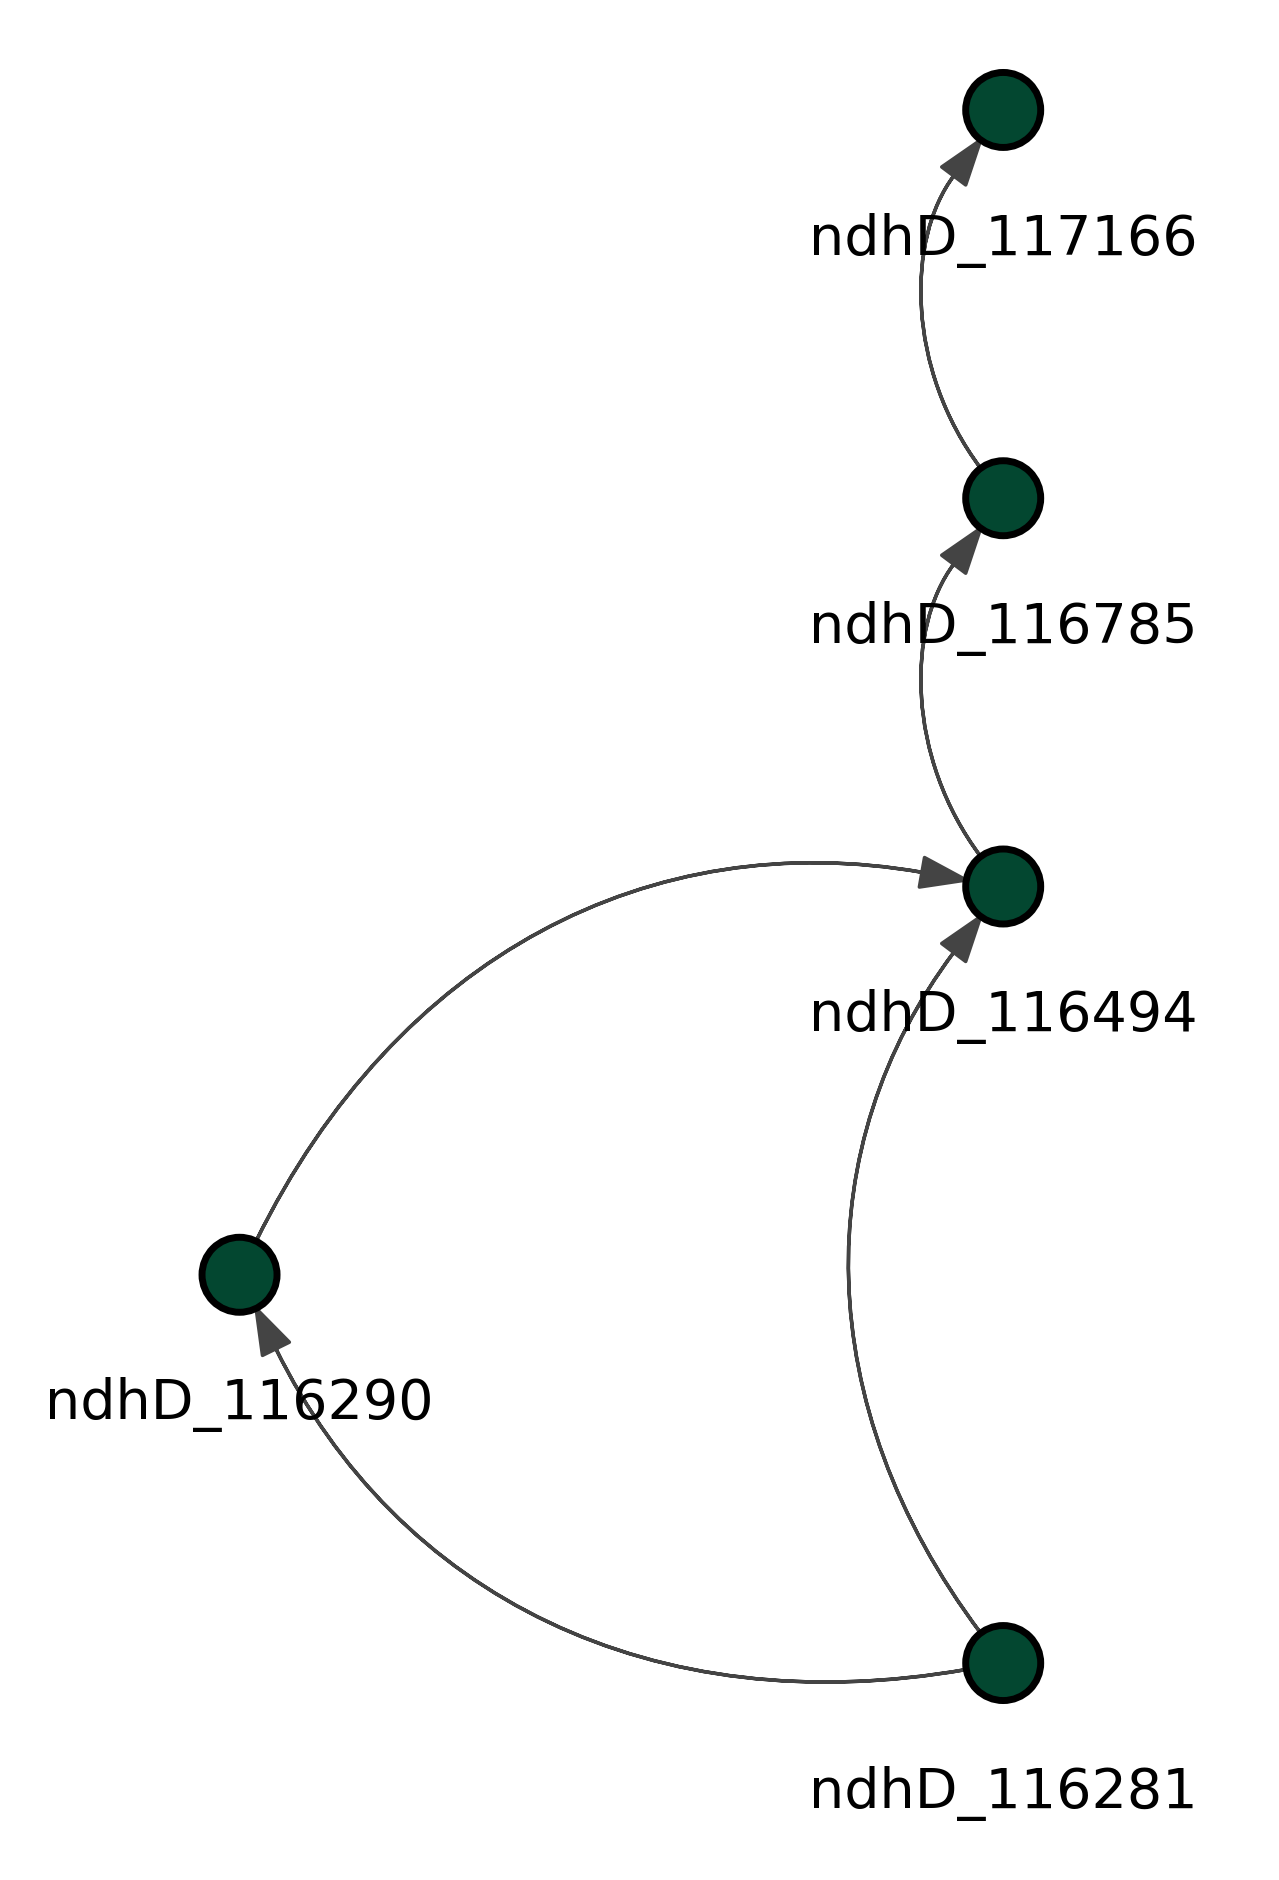
\includegraphics[width=3.125in,height=\textheight,keepaspectratio]{Figures Causal Discovery/DAG_NOTEARS_ndhD.png}

\subcaption{\label{}NOTEARS}
\end{minipage}%

\caption{\label{fig-CD_ndhD}Causal Discovery for \emph{ndhD}}

\end{figure}%

\subsubsection{Interventional reasoning}\label{sec-quant_CausalEffects}

Having identified directed edges through causal discovery, we now turn
to the question of whether these edges reflect true causal
relationships. To assess this, we apply \textbf{interventional
reasoning} using the \texttt{DoWhy} Python library
\citeproc{ref-dowhy}{{[}29{]}}, which enables us to estimate the
\textbf{Average Causal Effect (ACE)} of one event on another.

The \textbf{ACE} quantifies how much the outcome \(Y\) would change on
average if we were to intervene and set the treatment variable \(X\) to
1 versus 0. Formally, it is defined as

\[
\text{ACE} := \mathbb{E}[Y \mid \text{do}(X=1)] - \mathbb{E}[Y \mid \text{do}(X=0)].
\]

In situations where a mediator lies along the causal path from \(X\) to
\(Y\), we instead focus on estimating the Natural Direct Effect (NDE),
which captures the component of the effect not transmitted through the
mediator.

To carry out this analysis, we follow a structured four-step process for
each DAG learned from the data:

\begin{enumerate}
\def\labelenumi{\arabic{enumi}.}
\item
  \textbf{Model creation}. For each pair of events \((A, B)\) connected
  by a directed edge \(A \rightarrow B\), we construct a
  \texttt{CausalModel} in \texttt{DoWhy}, designating \(A\) as the
  treatment and \(B\) as the outcome.
\item
  \textbf{Identification}. Using the structure of the DAG,
  \texttt{DoWhy} checks whether the causal effect is identifiable from
  observational data. This step relies on graphical criteria such as the
  \textbf{backdoor} and \textbf{frontdoor} conditions derived from
  do-calculus.
\item
  \textbf{Estimation}. If the effect is identifiable, we estimate the
  ACE using statistical techniques such as linear regression or
  matching. When mediators are detected, the estimation is refined to
  isolate the NDE.
\item
  \textbf{Validation}. Finally, we retain only those causal links for
  which the estimated ACE is strictly positive, indicating a likely
  genuine causal influence. When an NDE is used, this value is reported
  instead. In both cases, the result is recorded in our summary tables
  under the label \emph{Actual Effect}.
\end{enumerate}

Full estimation details are provided in the appendix
Section~\ref{sec-causal_inference_results}, specifically in the
\emph{Causal relations figures} (Figure~\ref{fig-CR_ndhB} and
Figure~\ref{fig-CR_ndhD}), which present the most relevant causal
relationships inferred from each of the previously obtained graphs
together with the corresponding \emph{Actual Effect} value. We refer to
the available material at our
\href{https://github.com/cambroise/chloroDAG}{GitHub repository} for
further precisions.

\subsubsection{Chronology
representation}\label{chronology-representation}

The final step in our pipeline is \textbf{\emph{Chronology
representation}}: we construct the \emph{maximal causality path} based
on the previous analysis. Among all valid causal relationships estimated
previously, we retain only those with the highest impact in accordance
with the topological order of the discovered DAG. The construction of
the causal-chronology DAG is carried out in several steps.

\begin{enumerate}
\def\labelenumi{\roman{enumi}.}
\item
  We sort the rows of the causal inference tables in descending order of
  \emph{Actual Effect}.
\item
  Among the possible causes for the same `Outcome (Y)', we retain only
  the one with the greatest \emph{Actual Effect}. This yields a
  collection of \emph{high-impact} cause-effect arrows, which we refer
  to as \emph{strong\_causal\_relations}.
\item
  We compute the topological order of the discovered DAG and determine
  the level of each node. This is done using the
  \texttt{topological\_sorting()} function from the \texttt{igraph}
  Python library (cf. \citeproc{ref-igraphLibrary}{{[}30{]}}). The nodes
  are then grouped by their topological level.
\item
  We sort the directed edges in \emph{strong\_causal\_relations} in
  accordance with the topological levels of their source nodes.
\item
  We construct the corresponding DAG, thereby defining the chronology.
\item
  We verify whether all roots of the initial DAG are included in the
  chronology. If not, they are added as isolated nodes (at topological
  level \(0\)).
\item
  We add all nodes that were already isolated in the initial DAG as well
  as those that can become isolated after this construction.
\end{enumerate}

\begin{refremark}
Note that this construction implies that the resulting causal-chronology
DAG is a (directed) \emph{tree}. Indeed, in this procedure each node has
at most one incoming edge (since only the strongest causal link is
retained for each outcome) and cycles are prevented by the topological
ordering.

\label{rem-chron_tree}

\end{refremark}

The application of this method to the \emph{ndhB} and \emph{ndhD} genes
of the chloroplast of \emph{Arabidopsis thaliana} yields the maturation
timelines represented in their DAG form in Figure~\ref{fig-Chron_ndhB}
and Figure~\ref{fig-Chron_ndhD}, respectively.

\begin{figure}[H]

\begin{minipage}{0.43\linewidth}

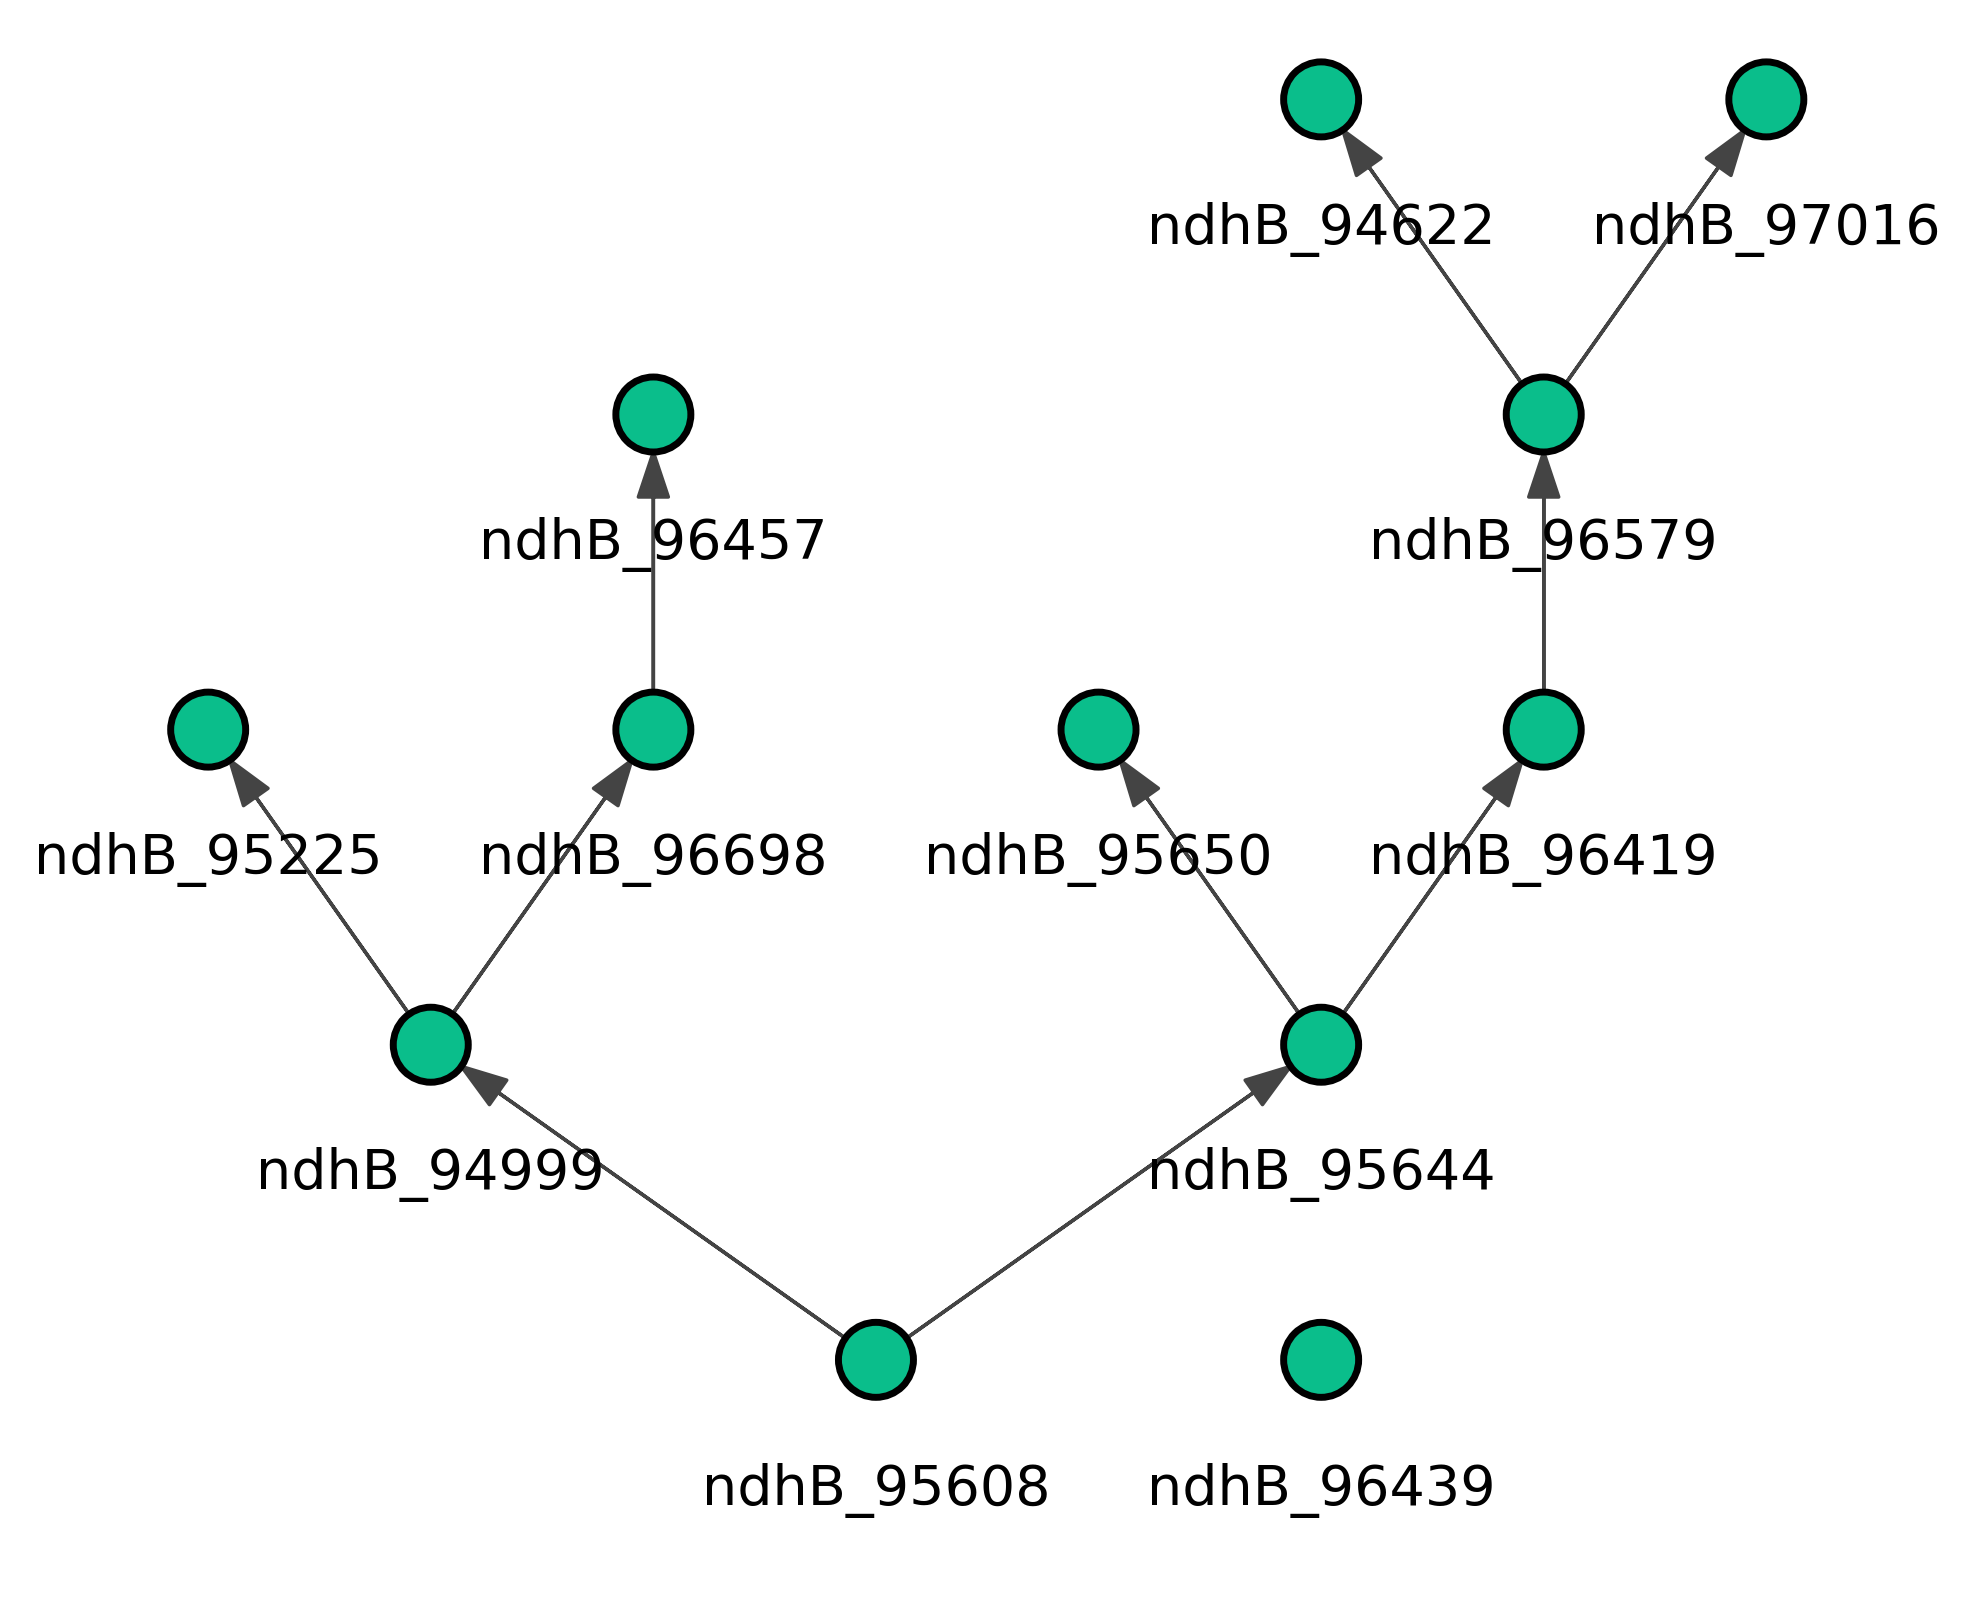
\includegraphics[width=3.125in,height=\textheight,keepaspectratio]{Figures Causal Chronology/chron_DAG_HC_ndhB.png}

\subcaption{\label{}HC-model}
\end{minipage}%
%
\begin{minipage}{0.13\linewidth}
~\end{minipage}%
%
\begin{minipage}{0.43\linewidth}

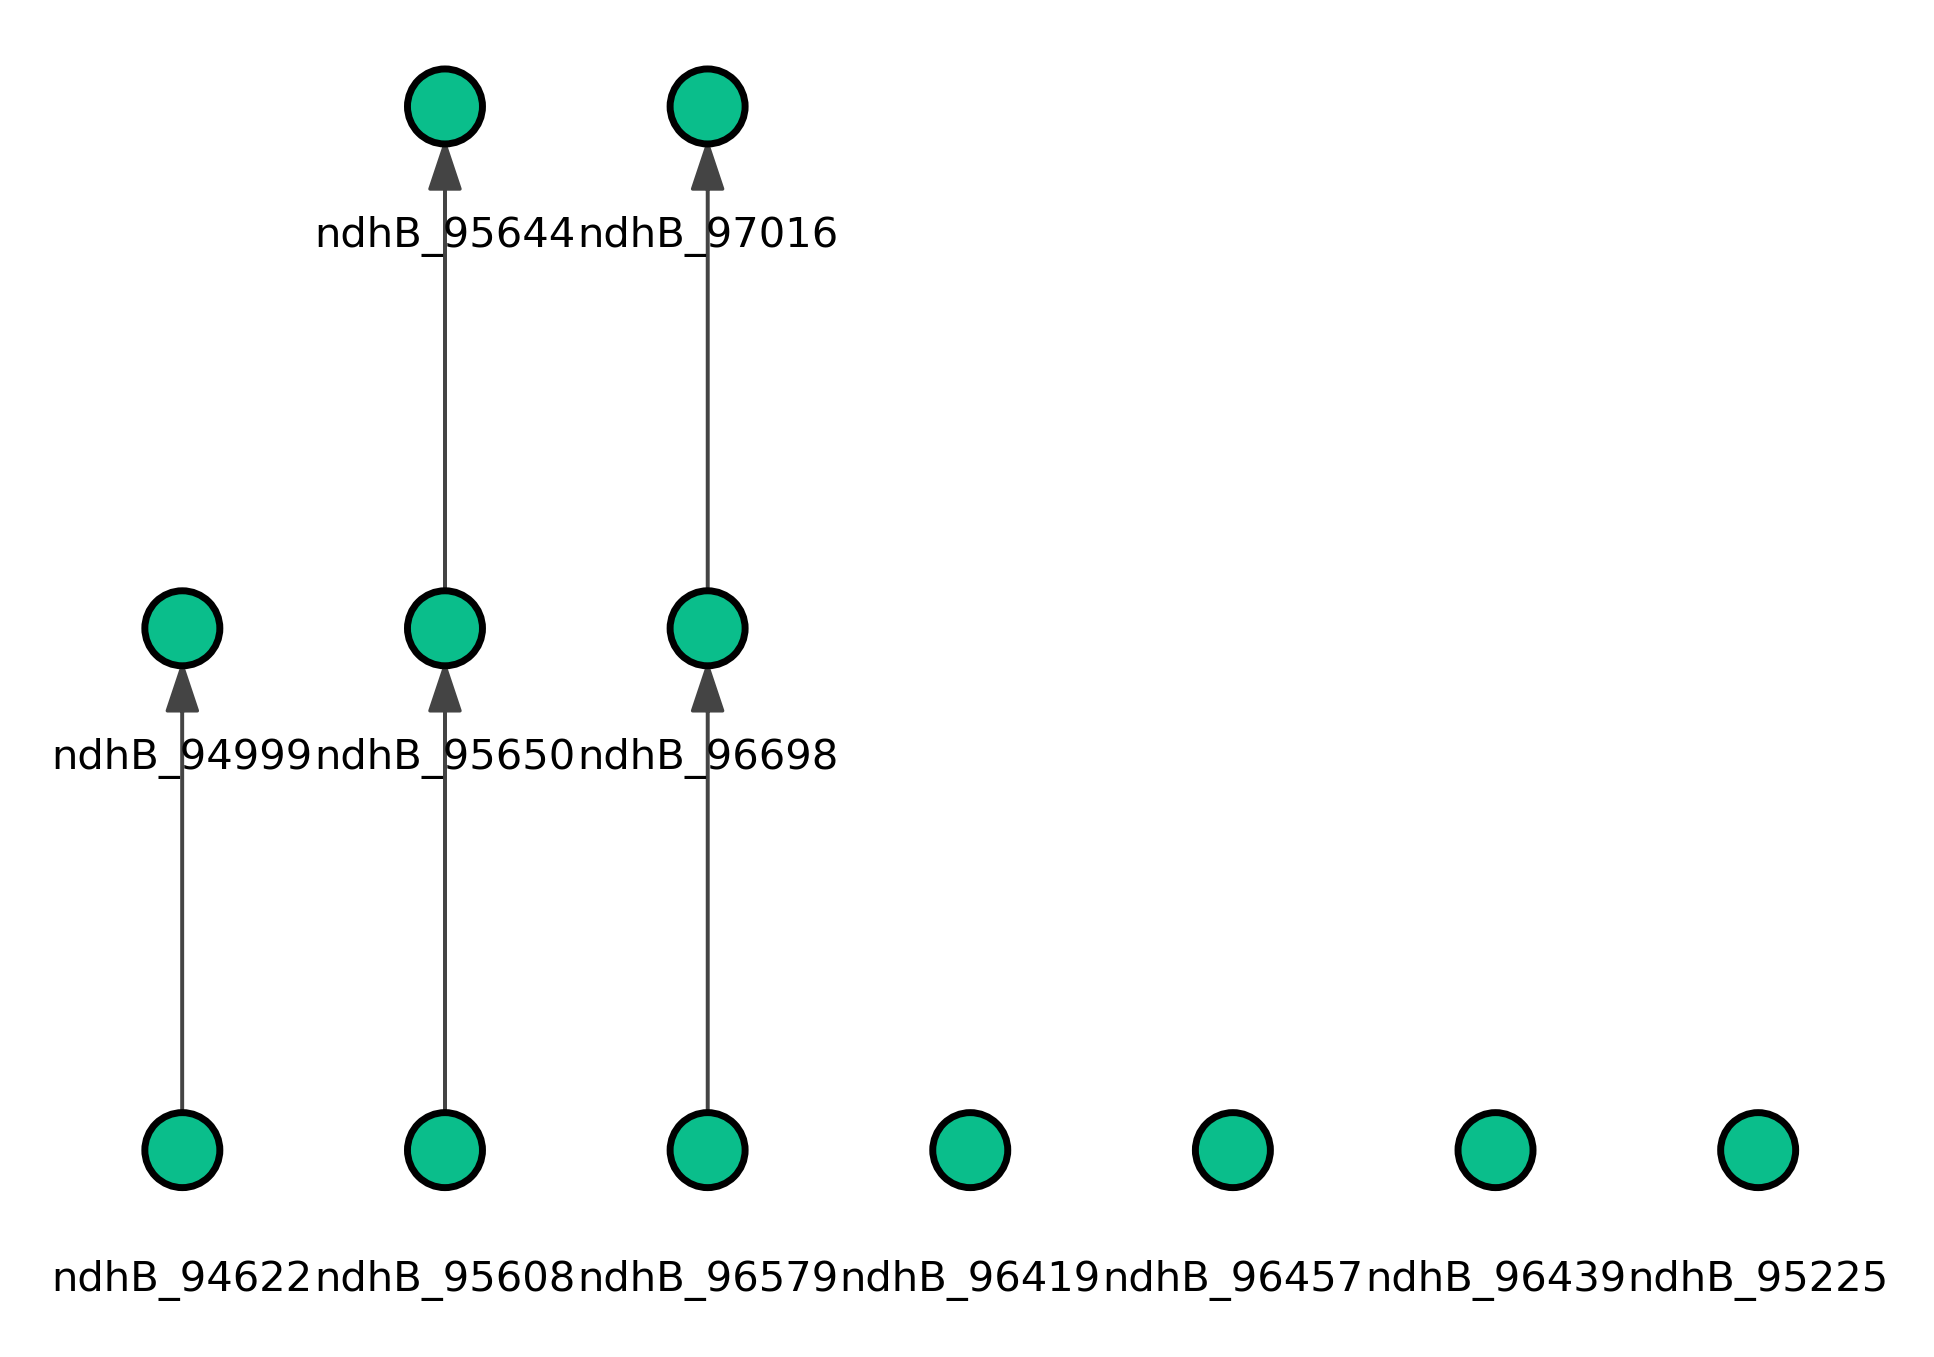
\includegraphics[width=3.125in,height=\textheight,keepaspectratio]{Figures Causal Chronology/chron_DAG_PC_ndhB.png}

\subcaption{\label{}PC-model}
\end{minipage}%
\newline
\begin{minipage}{0.43\linewidth}

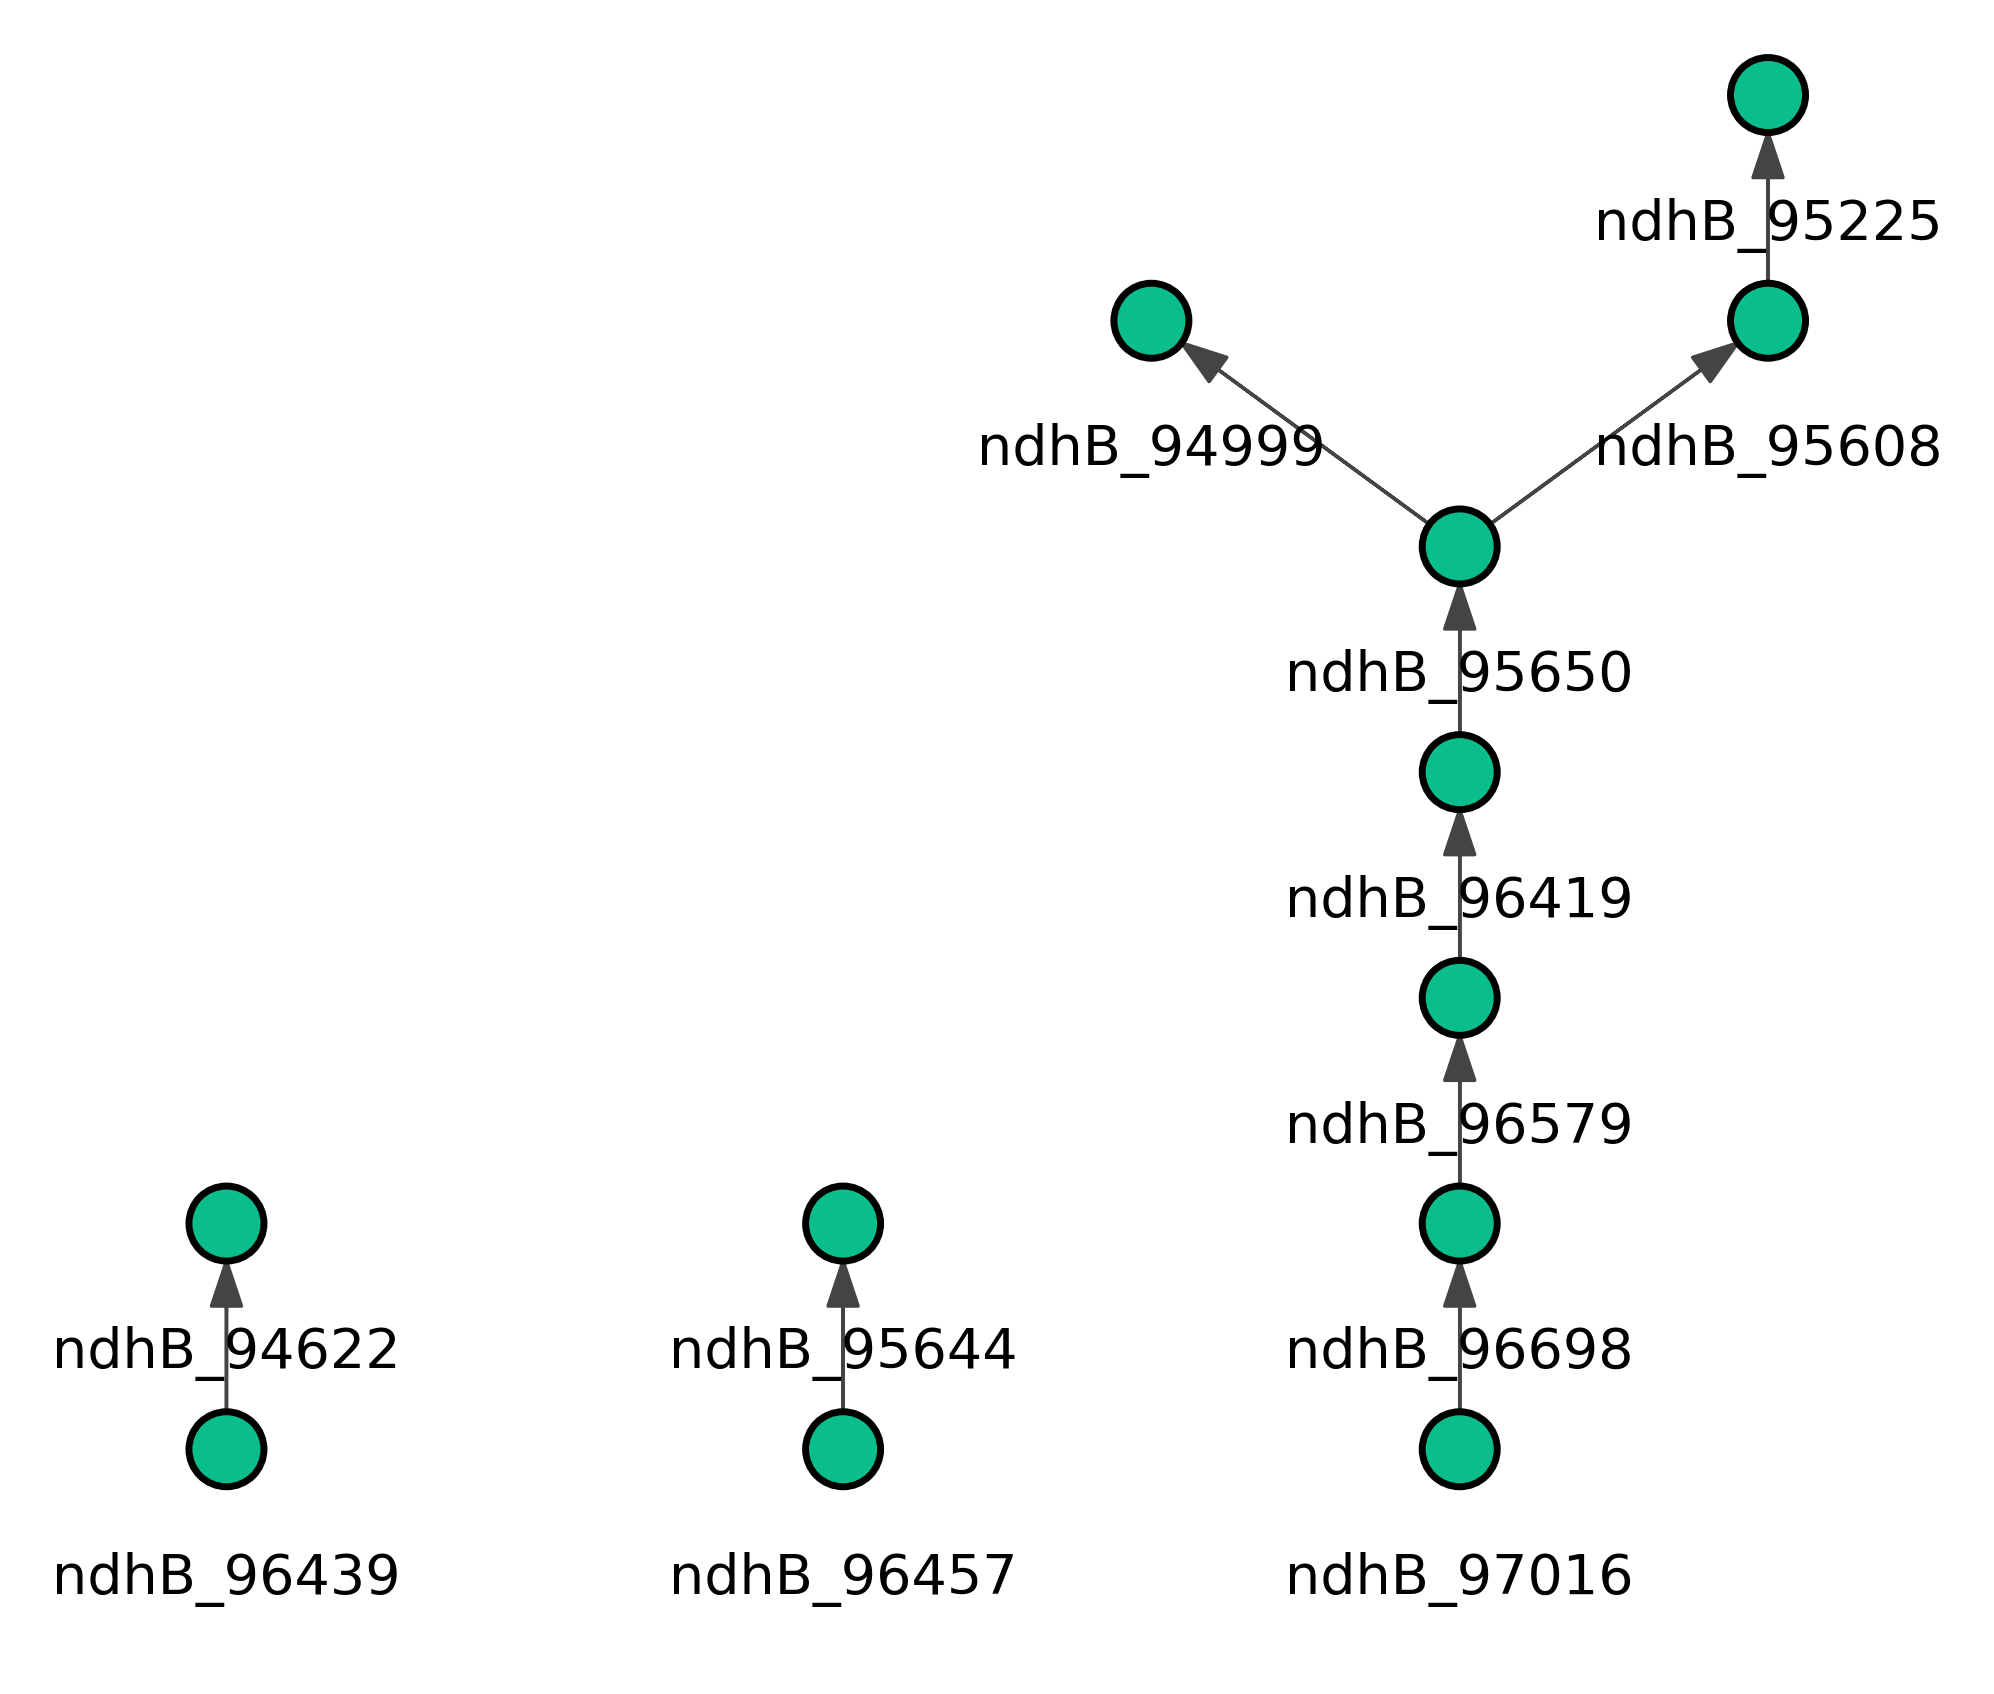
\includegraphics[width=3.125in,height=\textheight,keepaspectratio]{Figures Causal Chronology/chron_DAG_LiNGAM_ndhB.png}

\subcaption{\label{}LiNGAM-model}
\end{minipage}%
%
\begin{minipage}{0.13\linewidth}
~\end{minipage}%
%
\begin{minipage}{0.43\linewidth}

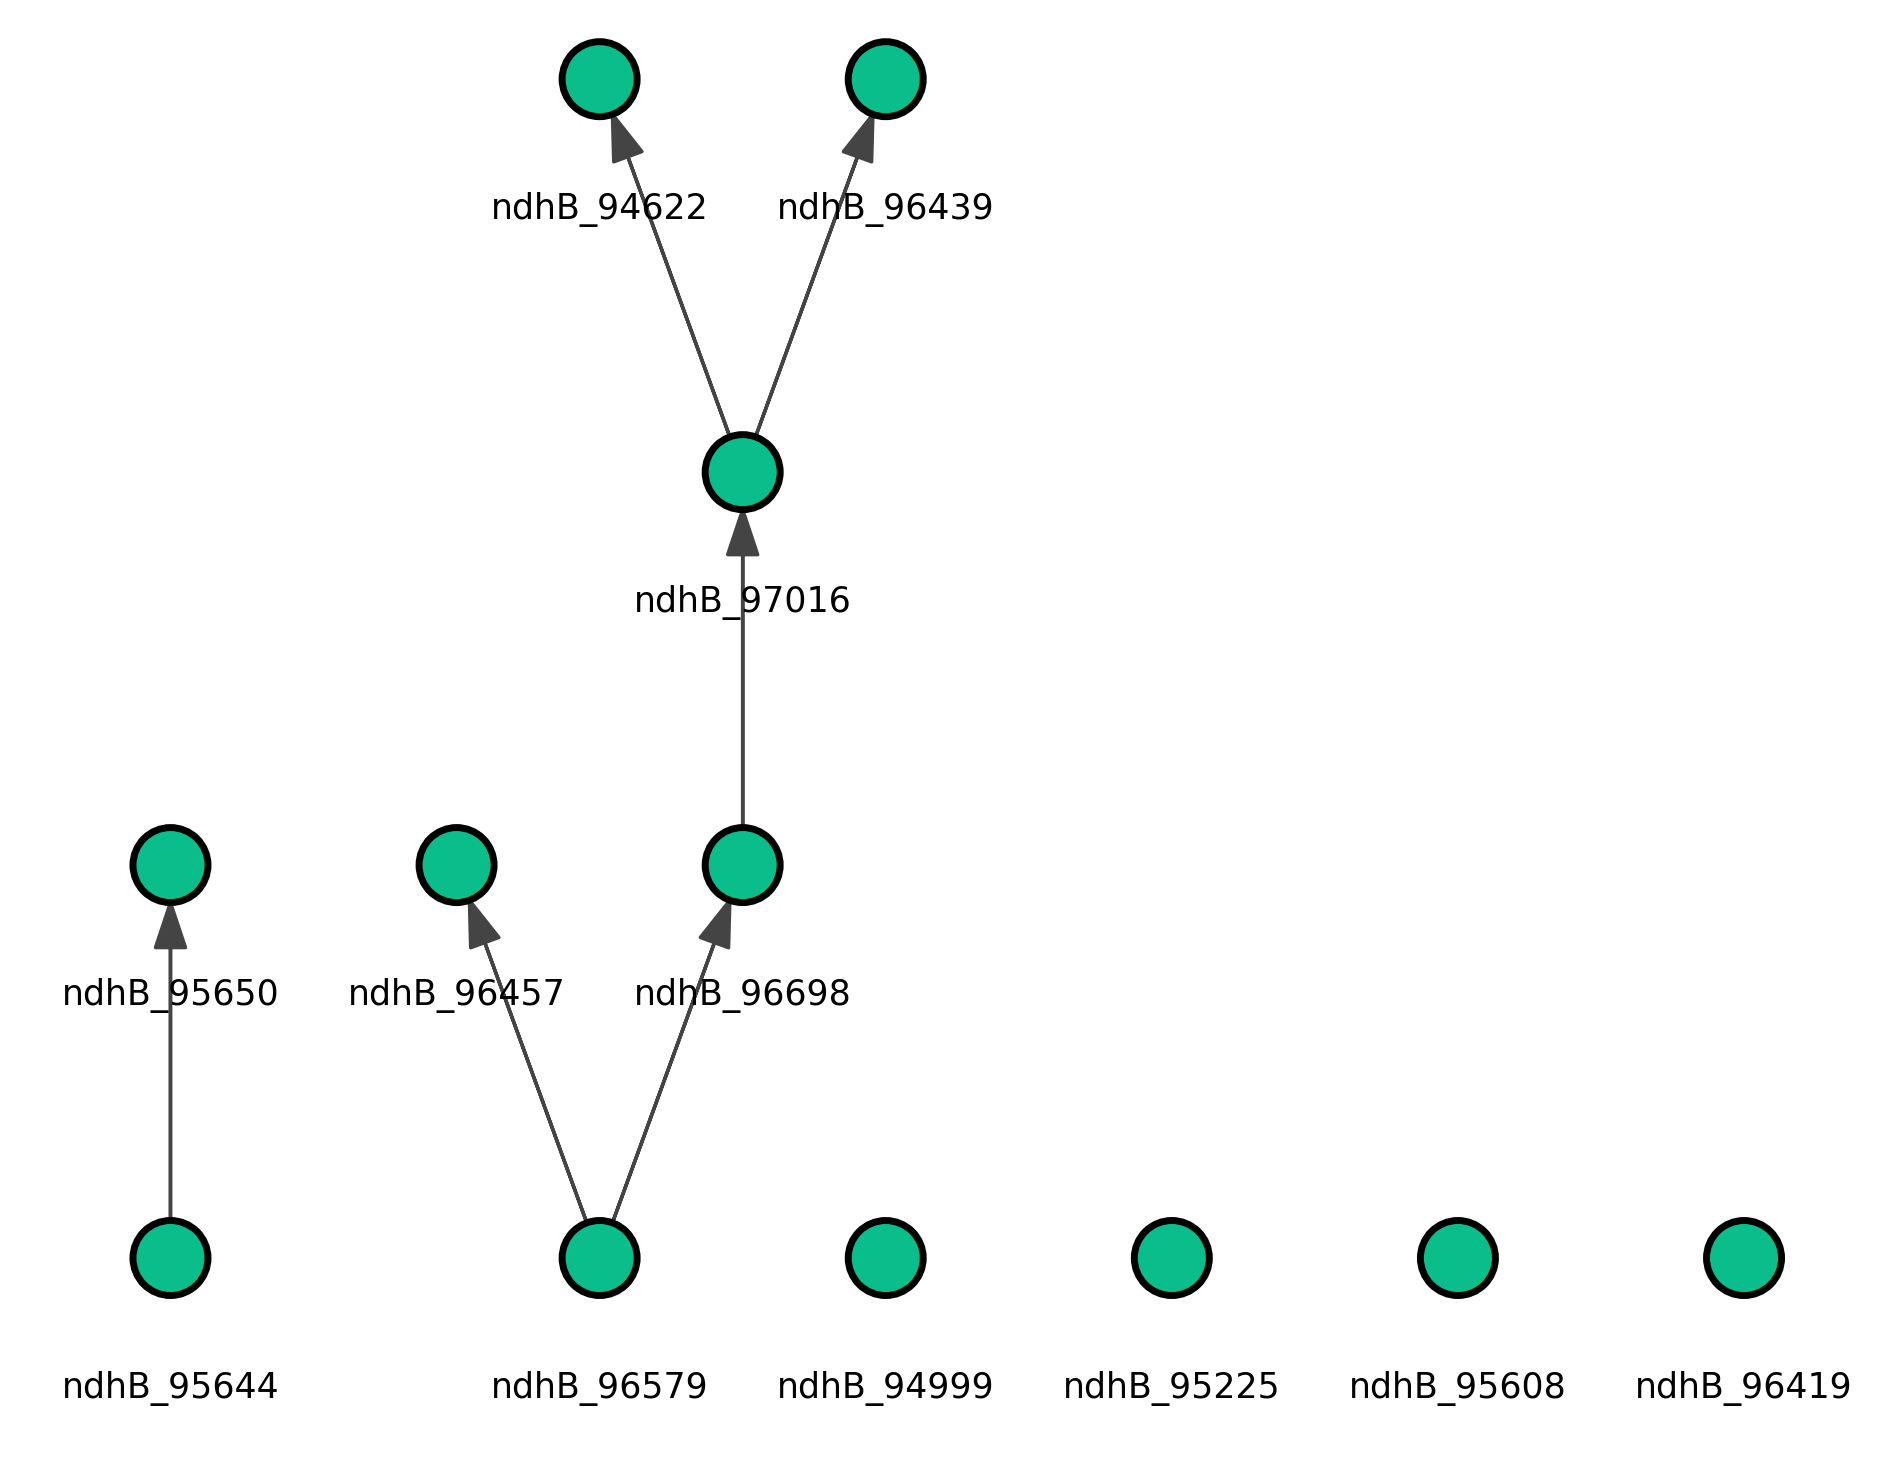
\includegraphics[width=3.125in,height=\textheight,keepaspectratio]{Figures Causal Chronology/chron_DAG_NOTEARS_ndhB.png}

\subcaption{\label{}NOTEARS-model}
\end{minipage}%

\caption{\label{fig-Chron_ndhB}Causal models for maturation chronology
for \emph{ndhB}}

\end{figure}%

\begin{figure}[H]

\begin{minipage}{0.43\linewidth}

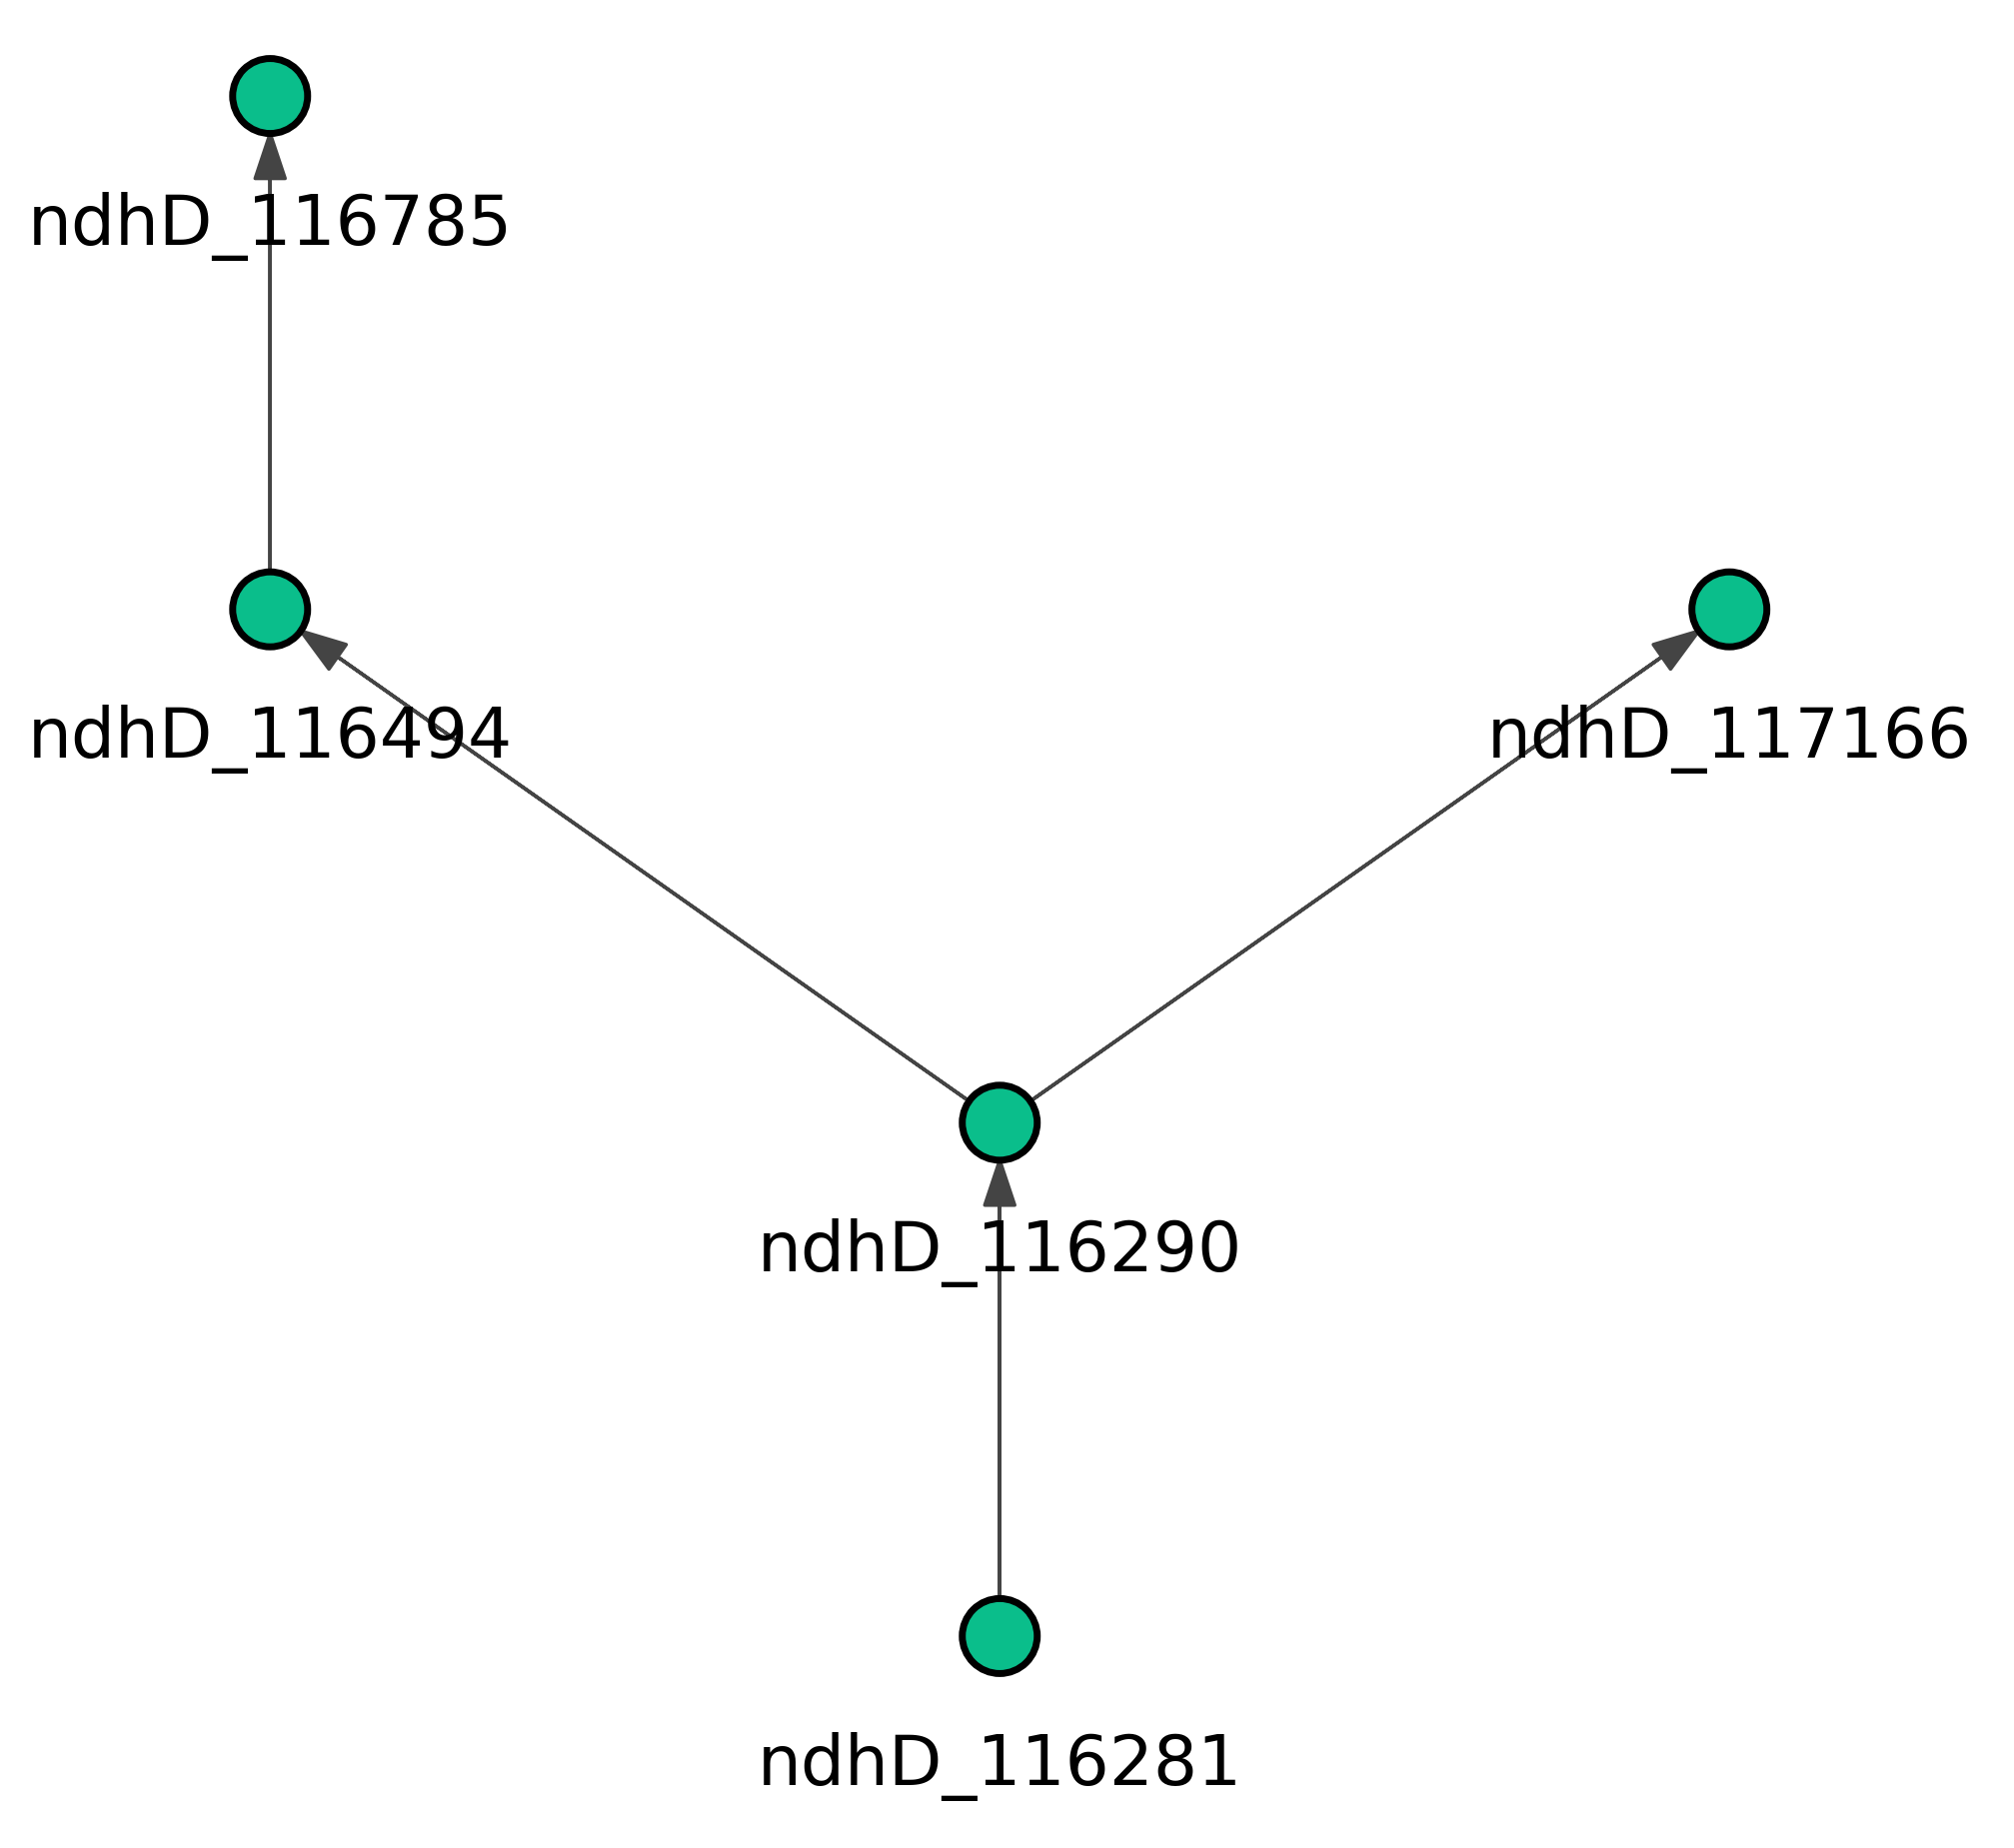
\includegraphics[width=3.125in,height=\textheight,keepaspectratio]{Figures Causal Chronology/chron_DAG_HC_ndhD.png}

\subcaption{\label{}HC-model}
\end{minipage}%
%
\begin{minipage}{0.13\linewidth}
~\end{minipage}%
%
\begin{minipage}{0.43\linewidth}

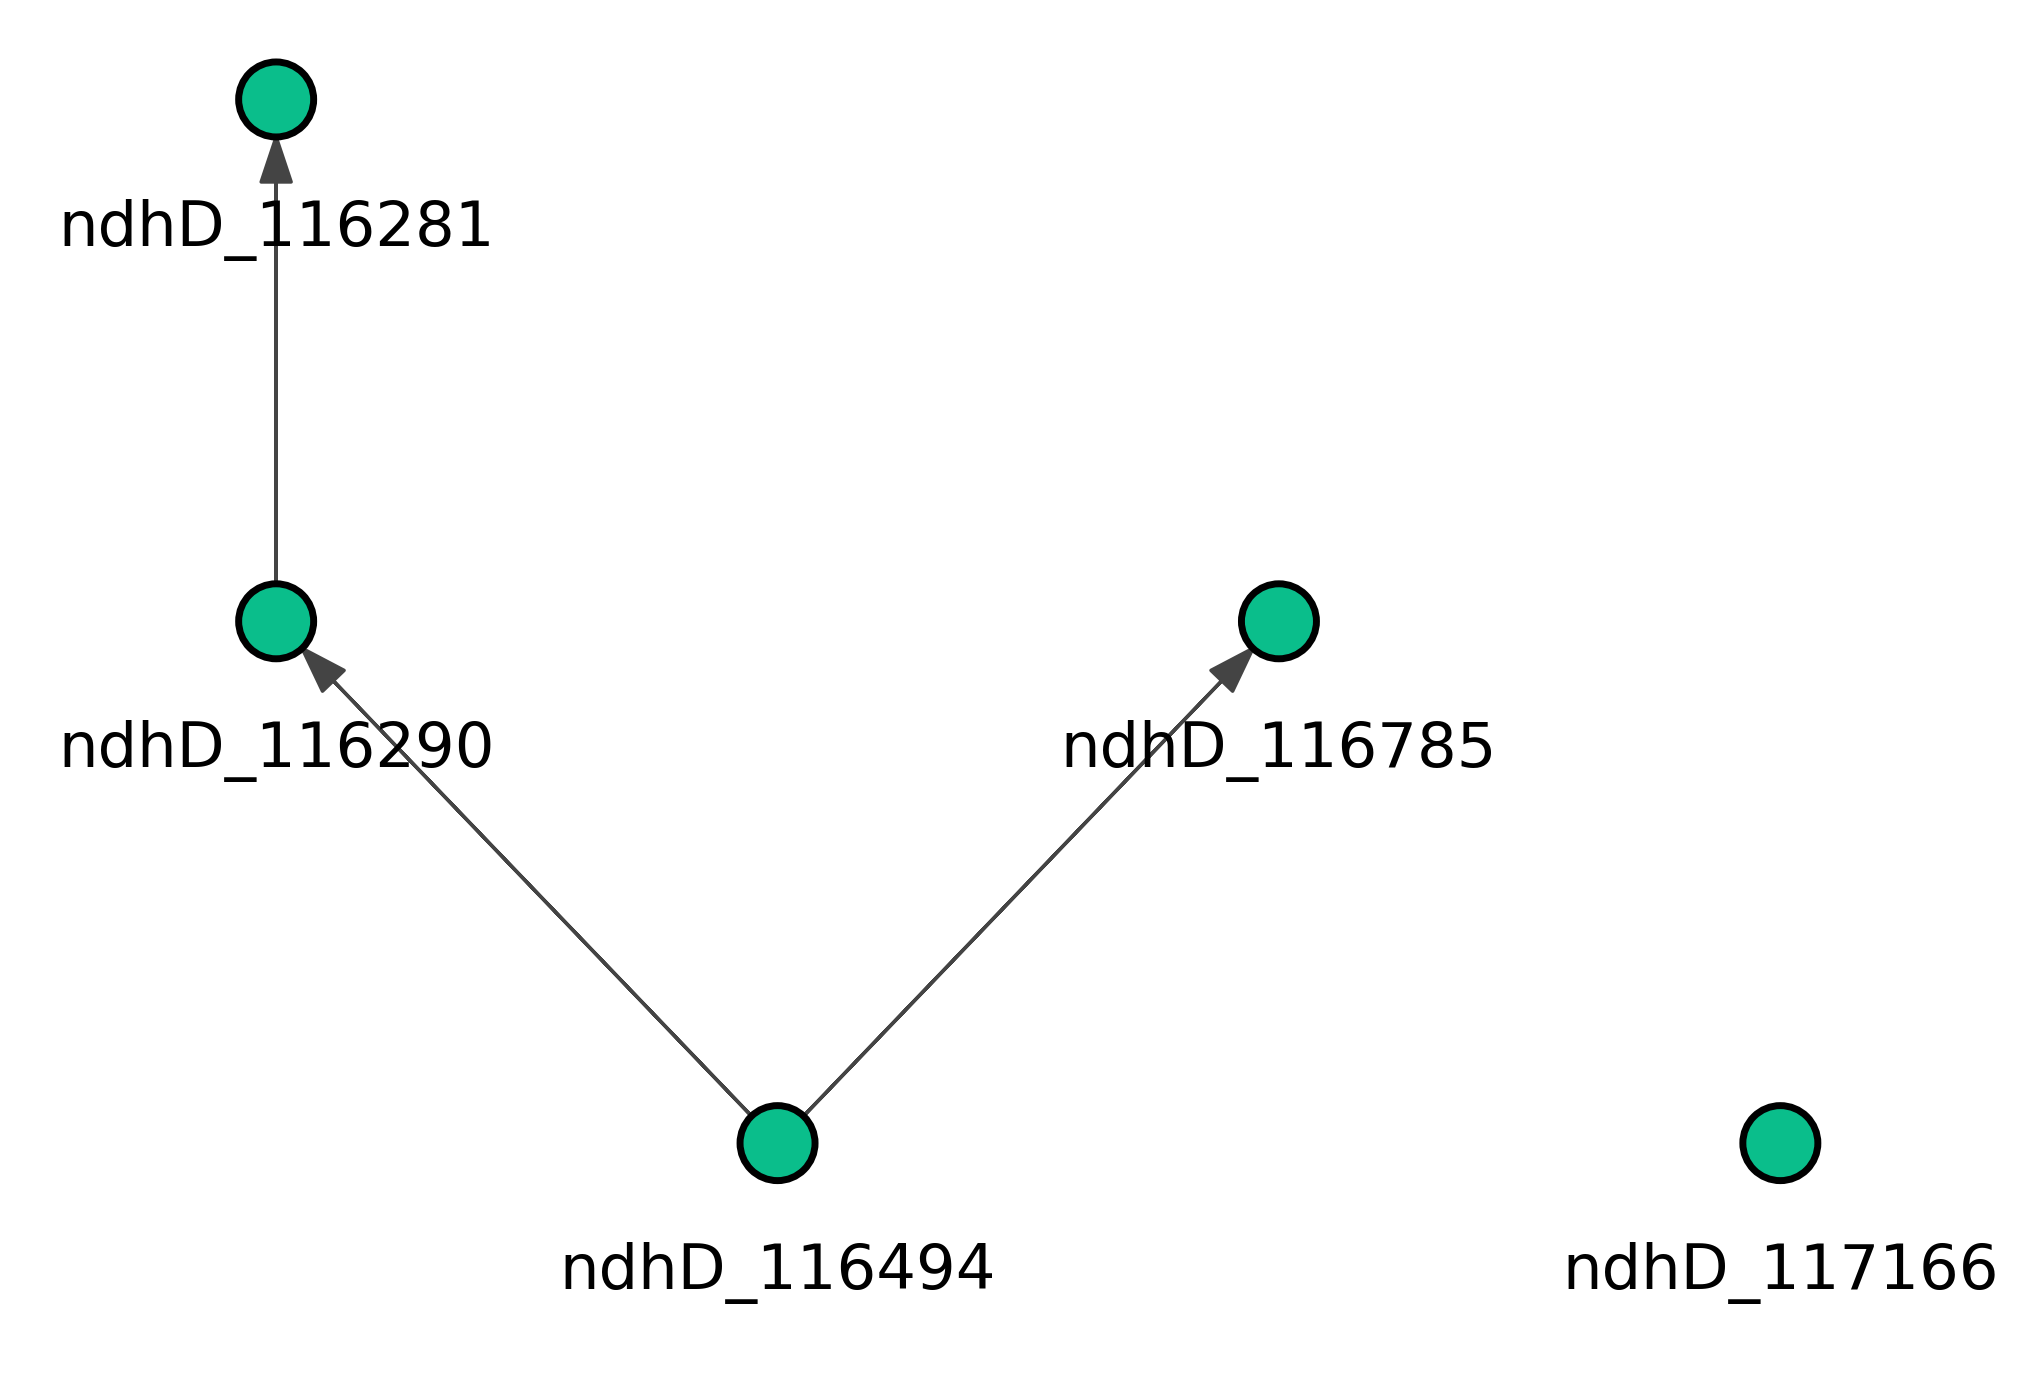
\includegraphics[width=3.125in,height=\textheight,keepaspectratio]{Figures Causal Chronology/chron_DAG_PC_ndhD.png}

\subcaption{\label{}PC-model}
\end{minipage}%
\newline
\begin{minipage}{0.43\linewidth}

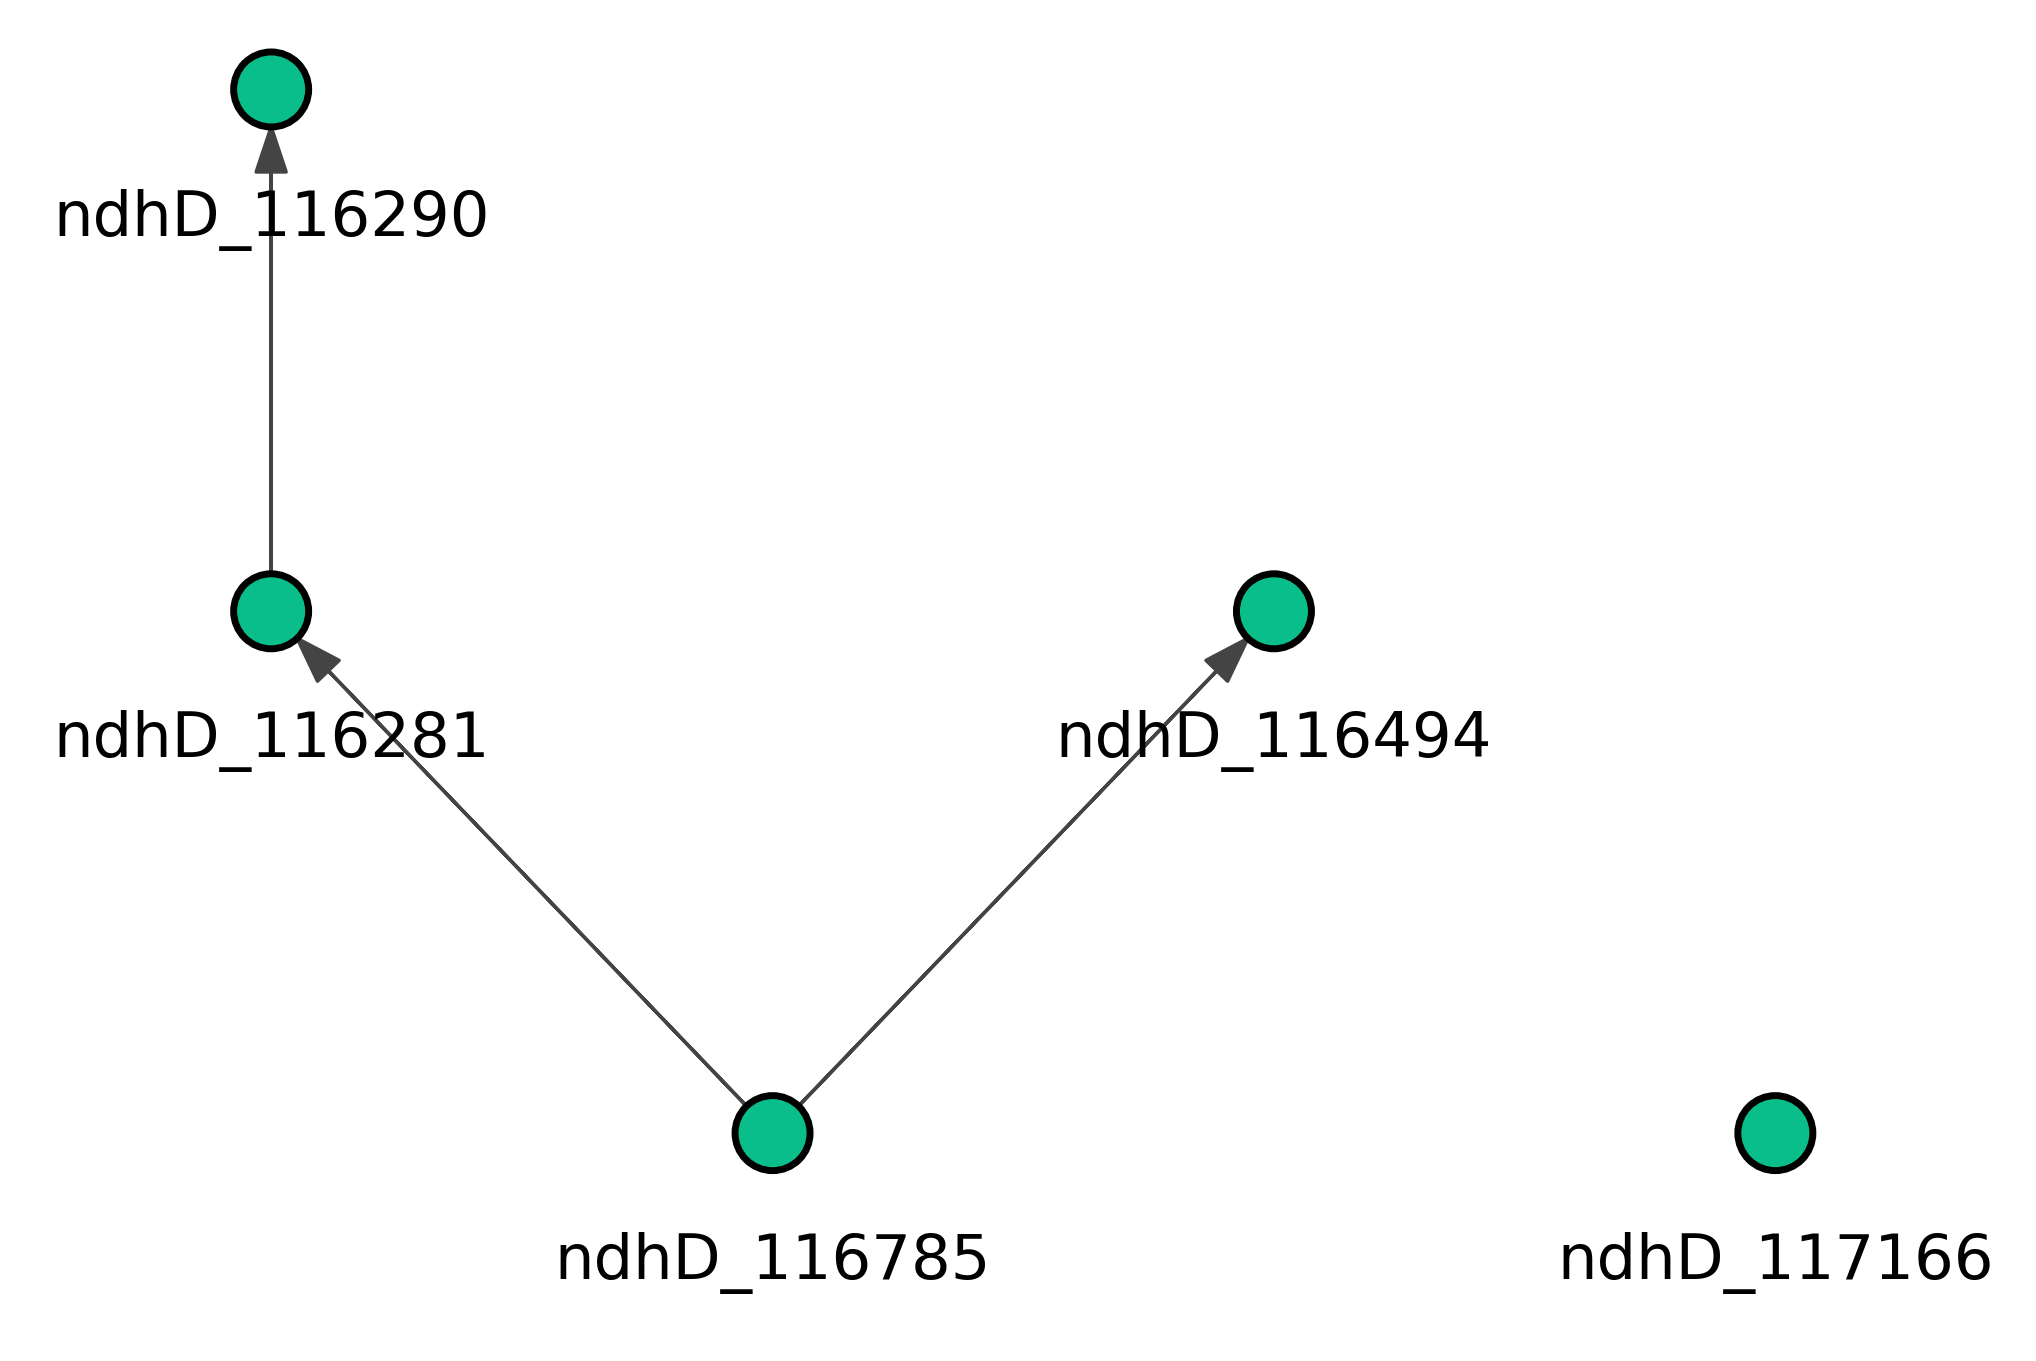
\includegraphics[width=3.125in,height=\textheight,keepaspectratio]{Figures Causal Chronology/chron_DAG_LiNGAM_ndhD.png}

\subcaption{\label{}LiNGAM-model}
\end{minipage}%
%
\begin{minipage}{0.13\linewidth}
~\end{minipage}%
%
\begin{minipage}{0.43\linewidth}

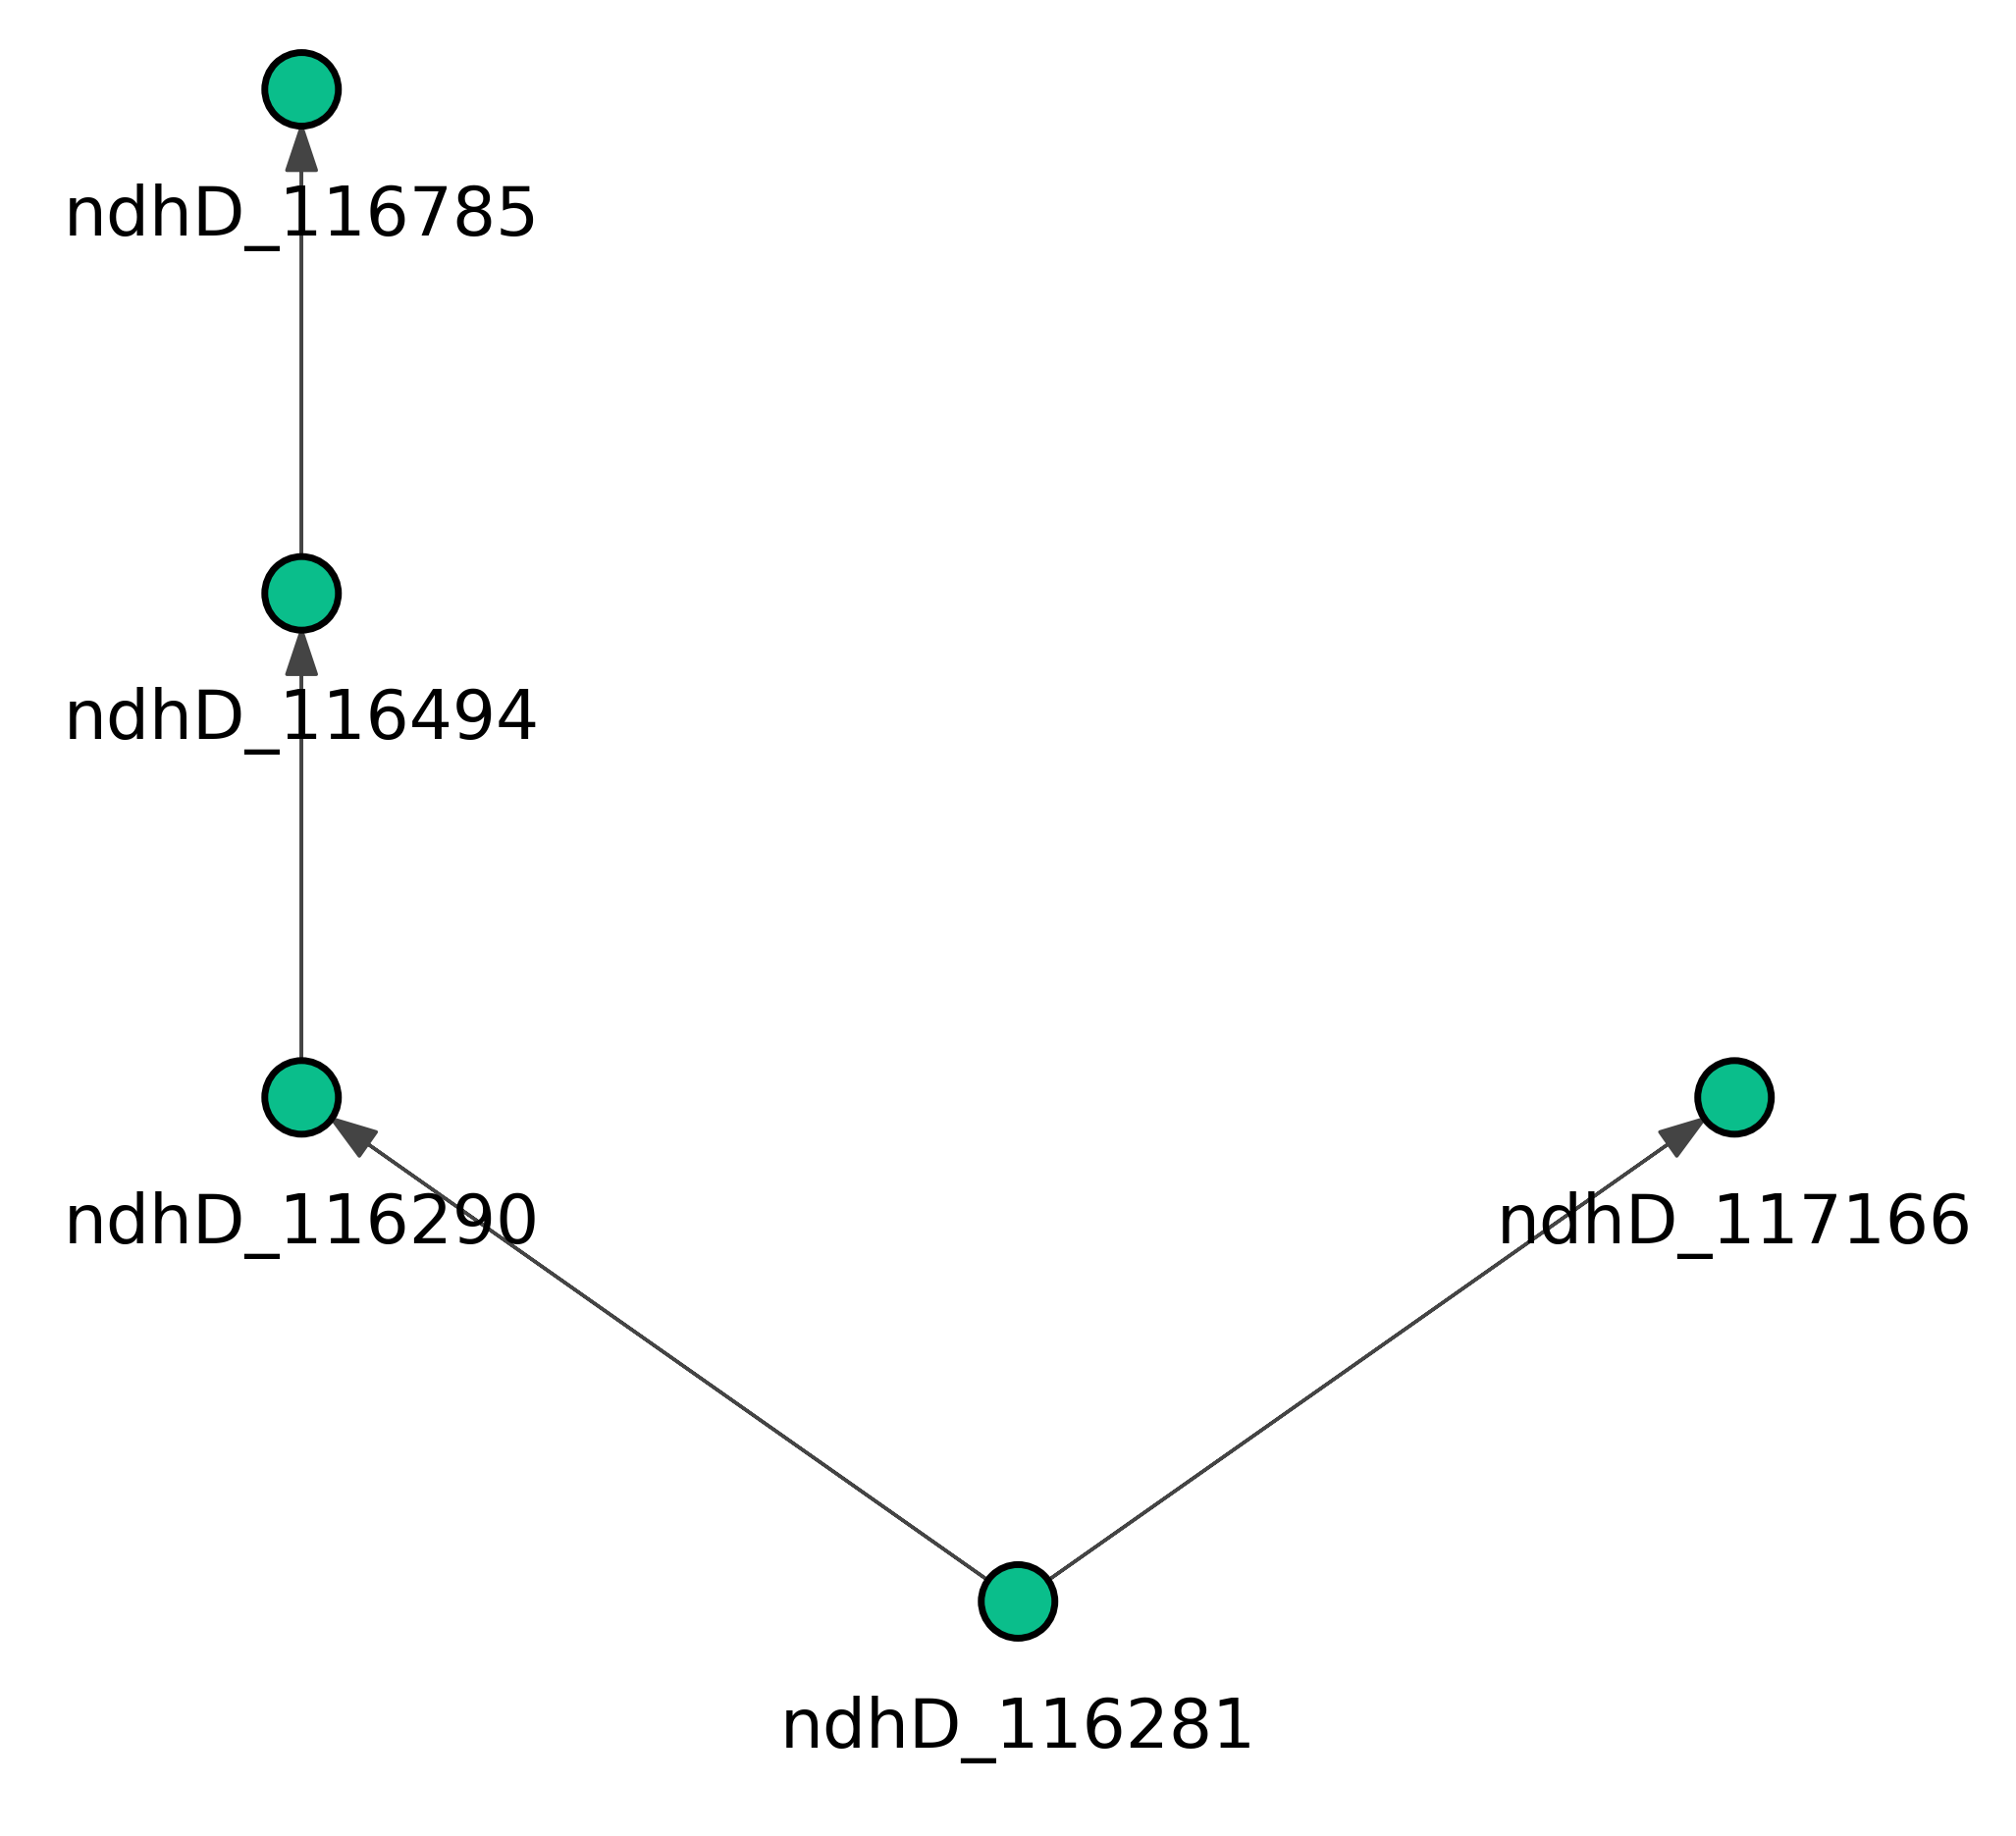
\includegraphics[width=3.125in,height=\textheight,keepaspectratio]{Figures Causal Chronology/chron_DAG_NOTEARS_ndhD.png}

\subcaption{\label{}NOTEARS-model}
\end{minipage}%

\caption{\label{fig-Chron_ndhD}Causal models for maturation chronology
for \emph{ndhD}}

\end{figure}%

These results naturally raise the question: \emph{which model should be
selected for a given gene?}

One approach is to validate each model against both the data and
existing expert knowledge. Details of this validation process ---
including assessments of the causal estimators and the inferred DAG
structures --- are provided in Section~\ref{sec-Reliability}.

Another complementary strategy is to perform a comparative analysis of
the inferred networks across multiple models, aiming to identify
\textbf{consistently recovered edges}. This consensus-based approach
highlights stable relationships---whether directed or undirected---that
appear robust to modeling choices. These consensus edges, combined with
expert knowledge, can then be used to define a \textbf{whitelist} of
trusted connections, guiding the construction of a more accurate and
interpretable regulatory network.

For example, the cross-analysis of the causal models for \emph{ndhB}
(Figure~\ref{fig-Chron_ndhB}) yields the sets of consistently recovered
directed and undirected edges represented in
Figure~\ref{fig-cross_analysis_ndhB} as a multigraph.

\begin{figure}[H]

\begin{minipage}{0.43\linewidth}

\centering{

\pandocbounded{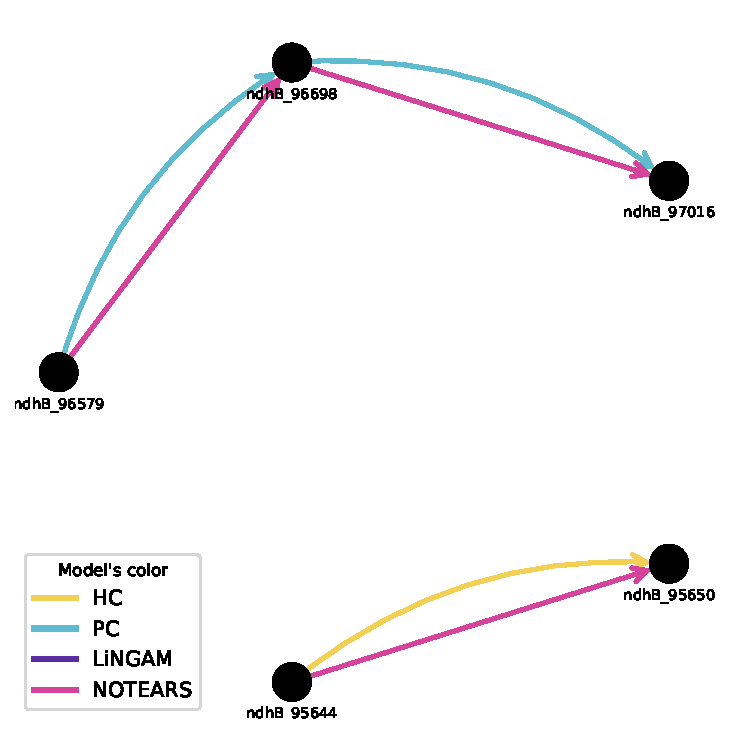
\includegraphics[keepaspectratio]{chloroDAG_files/figure-pdf/fig-cross_analysis_ndhb_dir-output-1.pdf}}

}

\subcaption{\label{fig-cross_analysis_ndhb_dir}Directed edges in at
least 2 models for \emph{ndhB}}

\end{minipage}%
%
\begin{minipage}{0.13\linewidth}
~\end{minipage}%
%
\begin{minipage}{0.43\linewidth}

\centering{

\pandocbounded{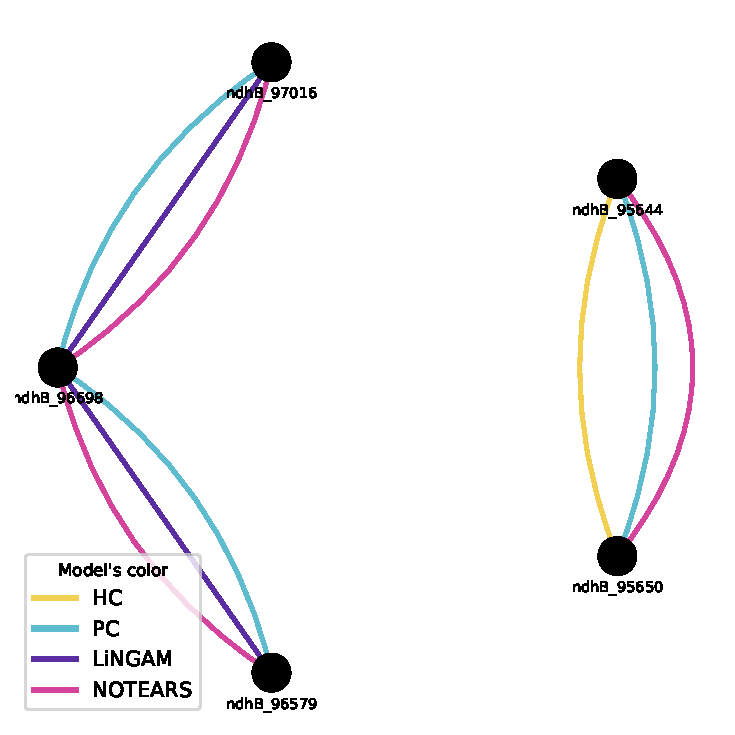
\includegraphics[keepaspectratio]{chloroDAG_files/figure-pdf/fig-cross_analysis_ndhb_undir-output-1.pdf}}

}

\subcaption{\label{fig-cross_analysis_ndhb_undir}Undirected edges in at
least 3 models for \emph{ndhB}}

\end{minipage}%

\caption{\label{fig-cross_analysis_ndhB}Cross-analysis for consistently
recovered edges within \emph{ndhB} causal models}

\end{figure}%

The cross-analysis of the causal models for \emph{ndhD}
(Figure~\ref{fig-Chron_ndhD}) yields the sets of consistently recovered
directed and undirected edges represented in
Figure~\ref{fig-cross_analysis_ndhD} as a multigraph.

\begin{figure}[H]

\begin{minipage}{0.43\linewidth}

\centering{

\pandocbounded{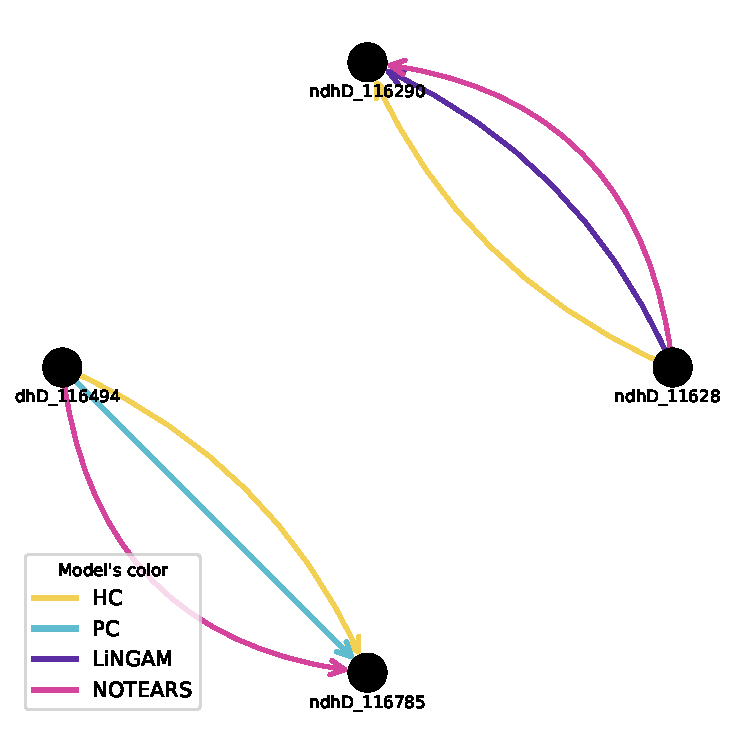
\includegraphics[keepaspectratio]{chloroDAG_files/figure-pdf/fig-cross_analysis_ndhd_dir-output-1.pdf}}

}

\subcaption{\label{fig-cross_analysis_ndhd_dir}Directed edges in at
least 3 models for \emph{ndhD}}

\end{minipage}%
%
\begin{minipage}{0.13\linewidth}
~\end{minipage}%
%
\begin{minipage}{0.43\linewidth}

\centering{

\pandocbounded{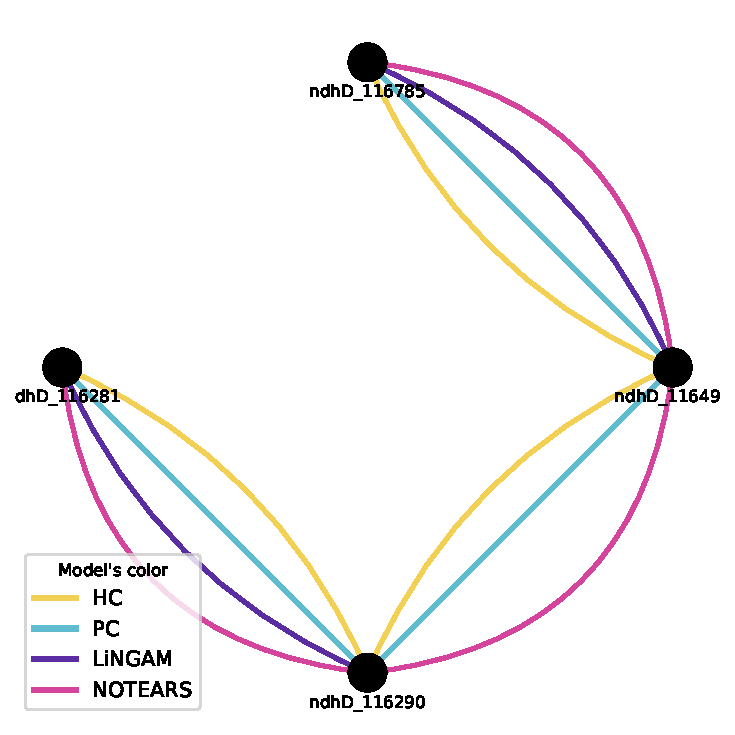
\includegraphics[keepaspectratio]{chloroDAG_files/figure-pdf/fig-cross_analysis_ndhd_undir-output-1.pdf}}

}

\subcaption{\label{fig-cross_analysis_ndhd_undir}Undirected edges in at
least 3 models for \emph{ndhD}}

\end{minipage}%

\caption{\label{fig-cross_analysis_ndhD}Cross-analysis for consistently
recovered edges within \emph{ndhD} causal models}

\end{figure}%

\subsubsection{Comparison with Reference
Models}\label{comparison-with-reference-models}

We next compare our inferred maturation timelines with the reference
chronologies presented by Guilcher \emph{et al.}
\citeproc{ref-Long_Reads_GuilcherEtAl}{{[}1{]}} to assess whether the
causal-chronology models provide a superior fit to the observed
maturation process.

The reference timelines for \emph{ndhB} and \emph{ndhD}, as defined in
\citeproc{ref-Long_Reads_GuilcherEtAl}{{[}1{]}}, are illustrated in DAG
form in Figure~\ref{fig-ref_chrons}.

\begin{figure}[H]

\begin{minipage}{0.43\linewidth}

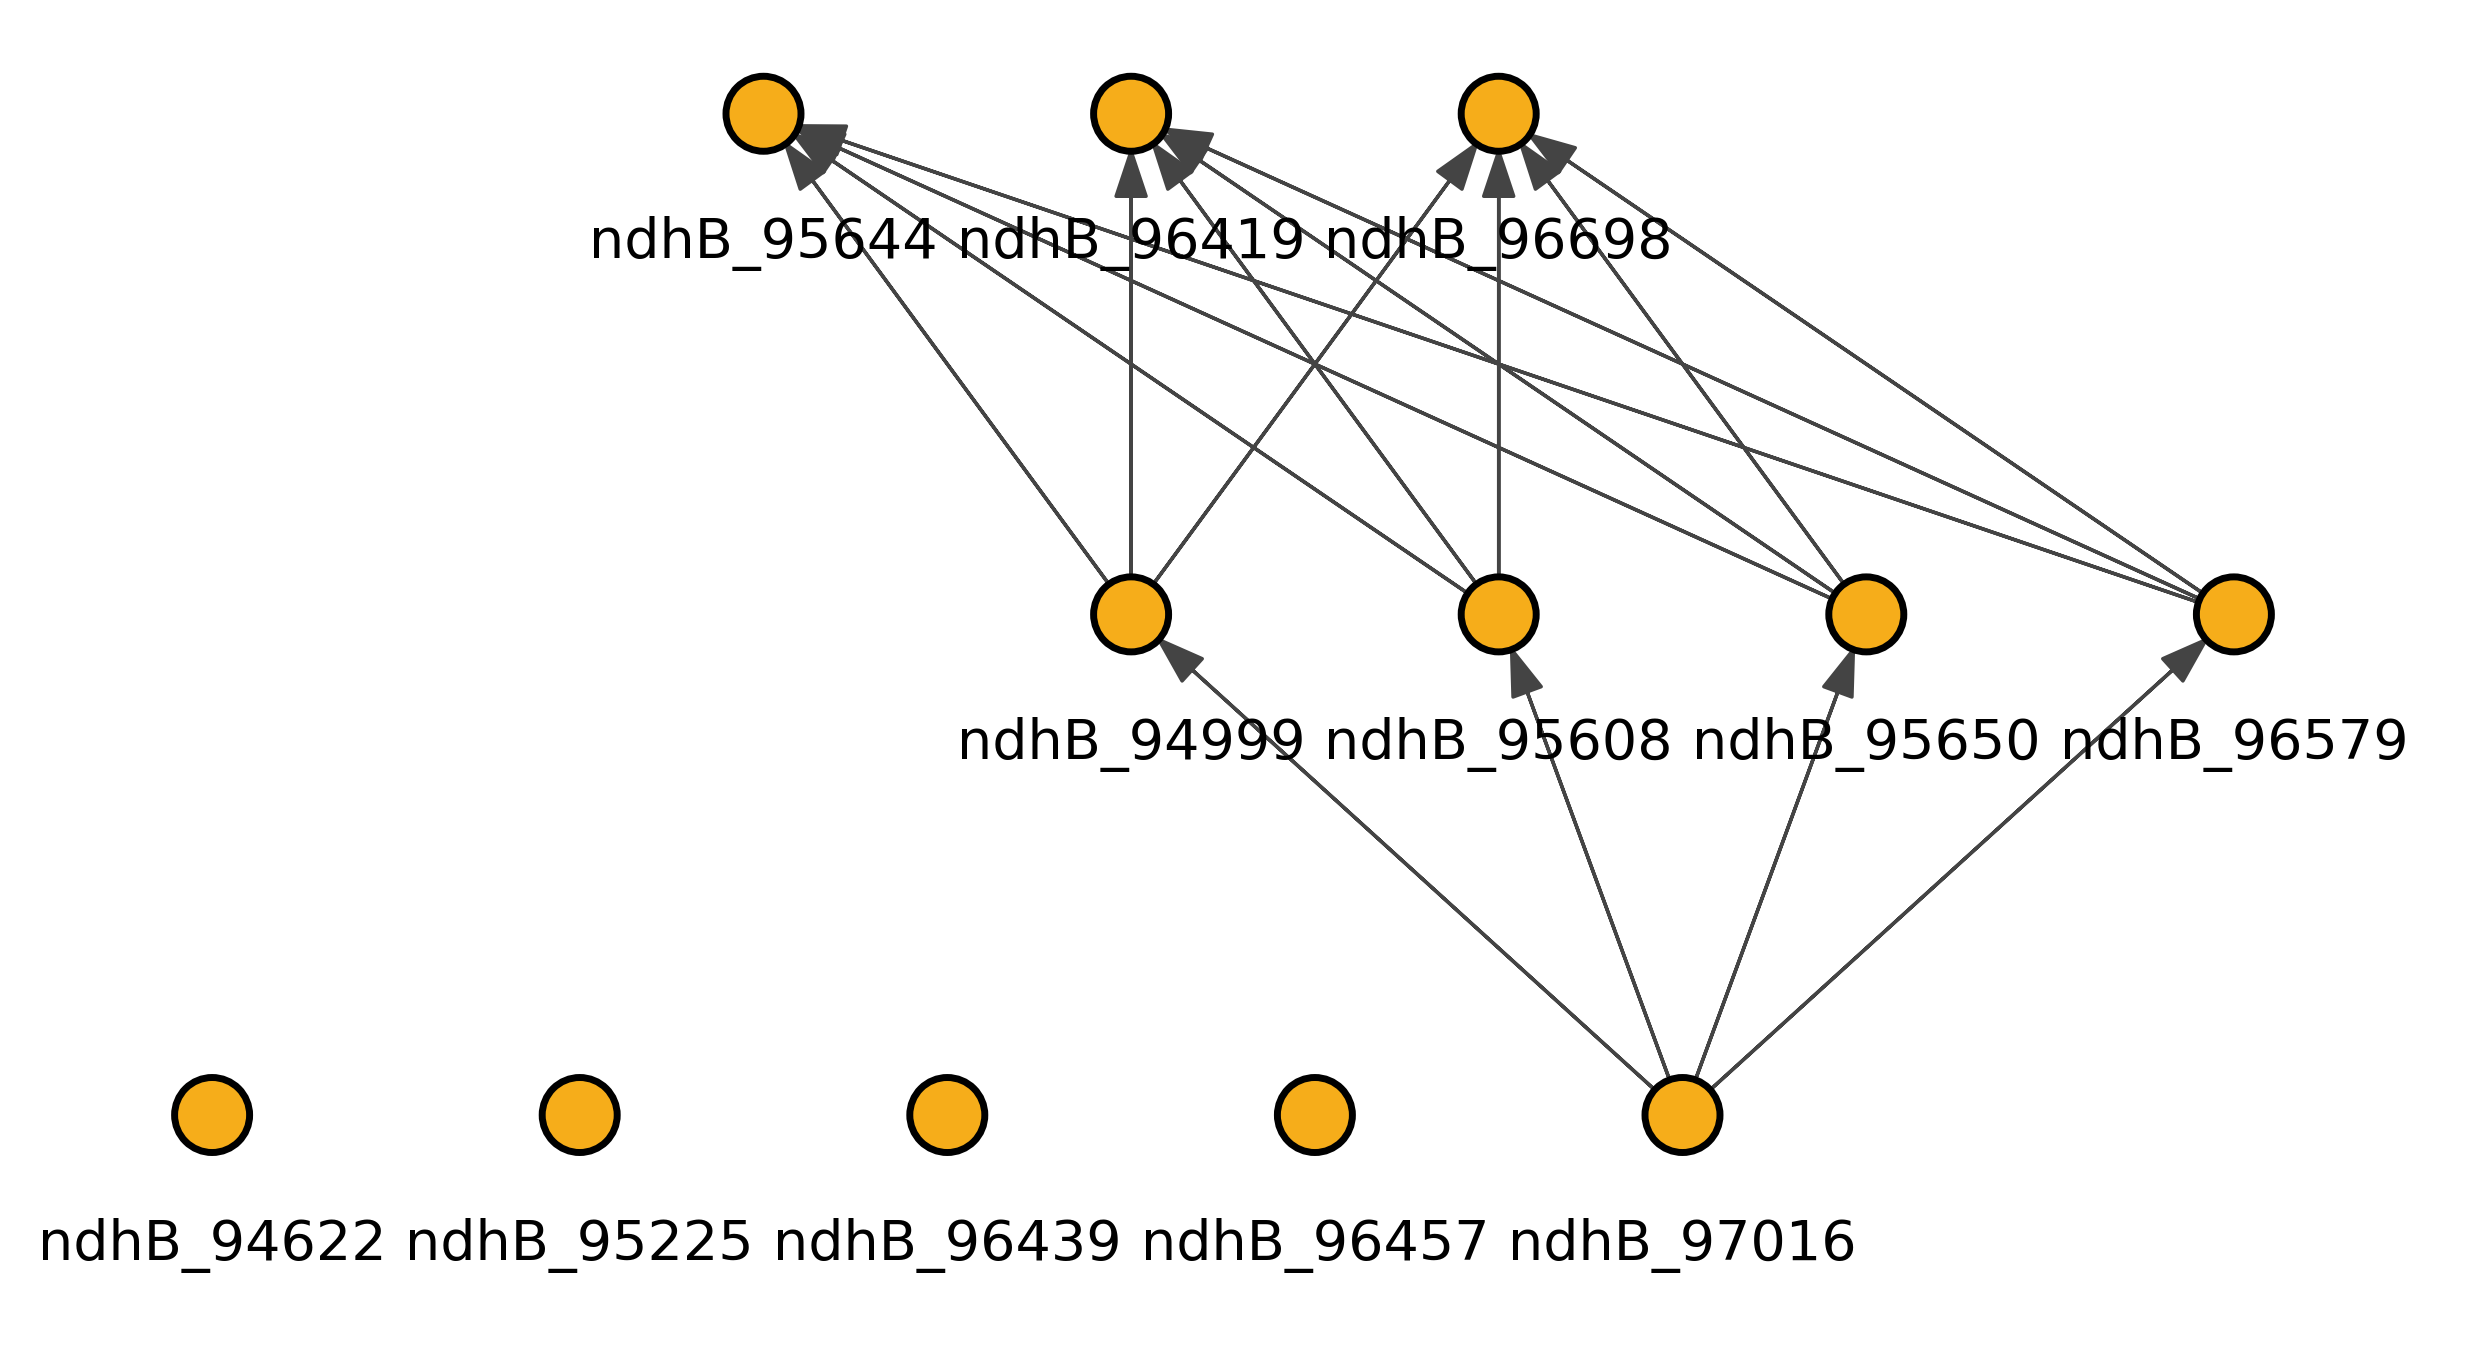
\includegraphics[width=3.125in,height=\textheight,keepaspectratio]{Figures Reference Graphs/chron_ndhB_Fig6_without_intron.png}

\subcaption{\label{}\emph{ndhB}}
\end{minipage}%
%
\begin{minipage}{0.13\linewidth}
~\end{minipage}%
%
\begin{minipage}{0.43\linewidth}

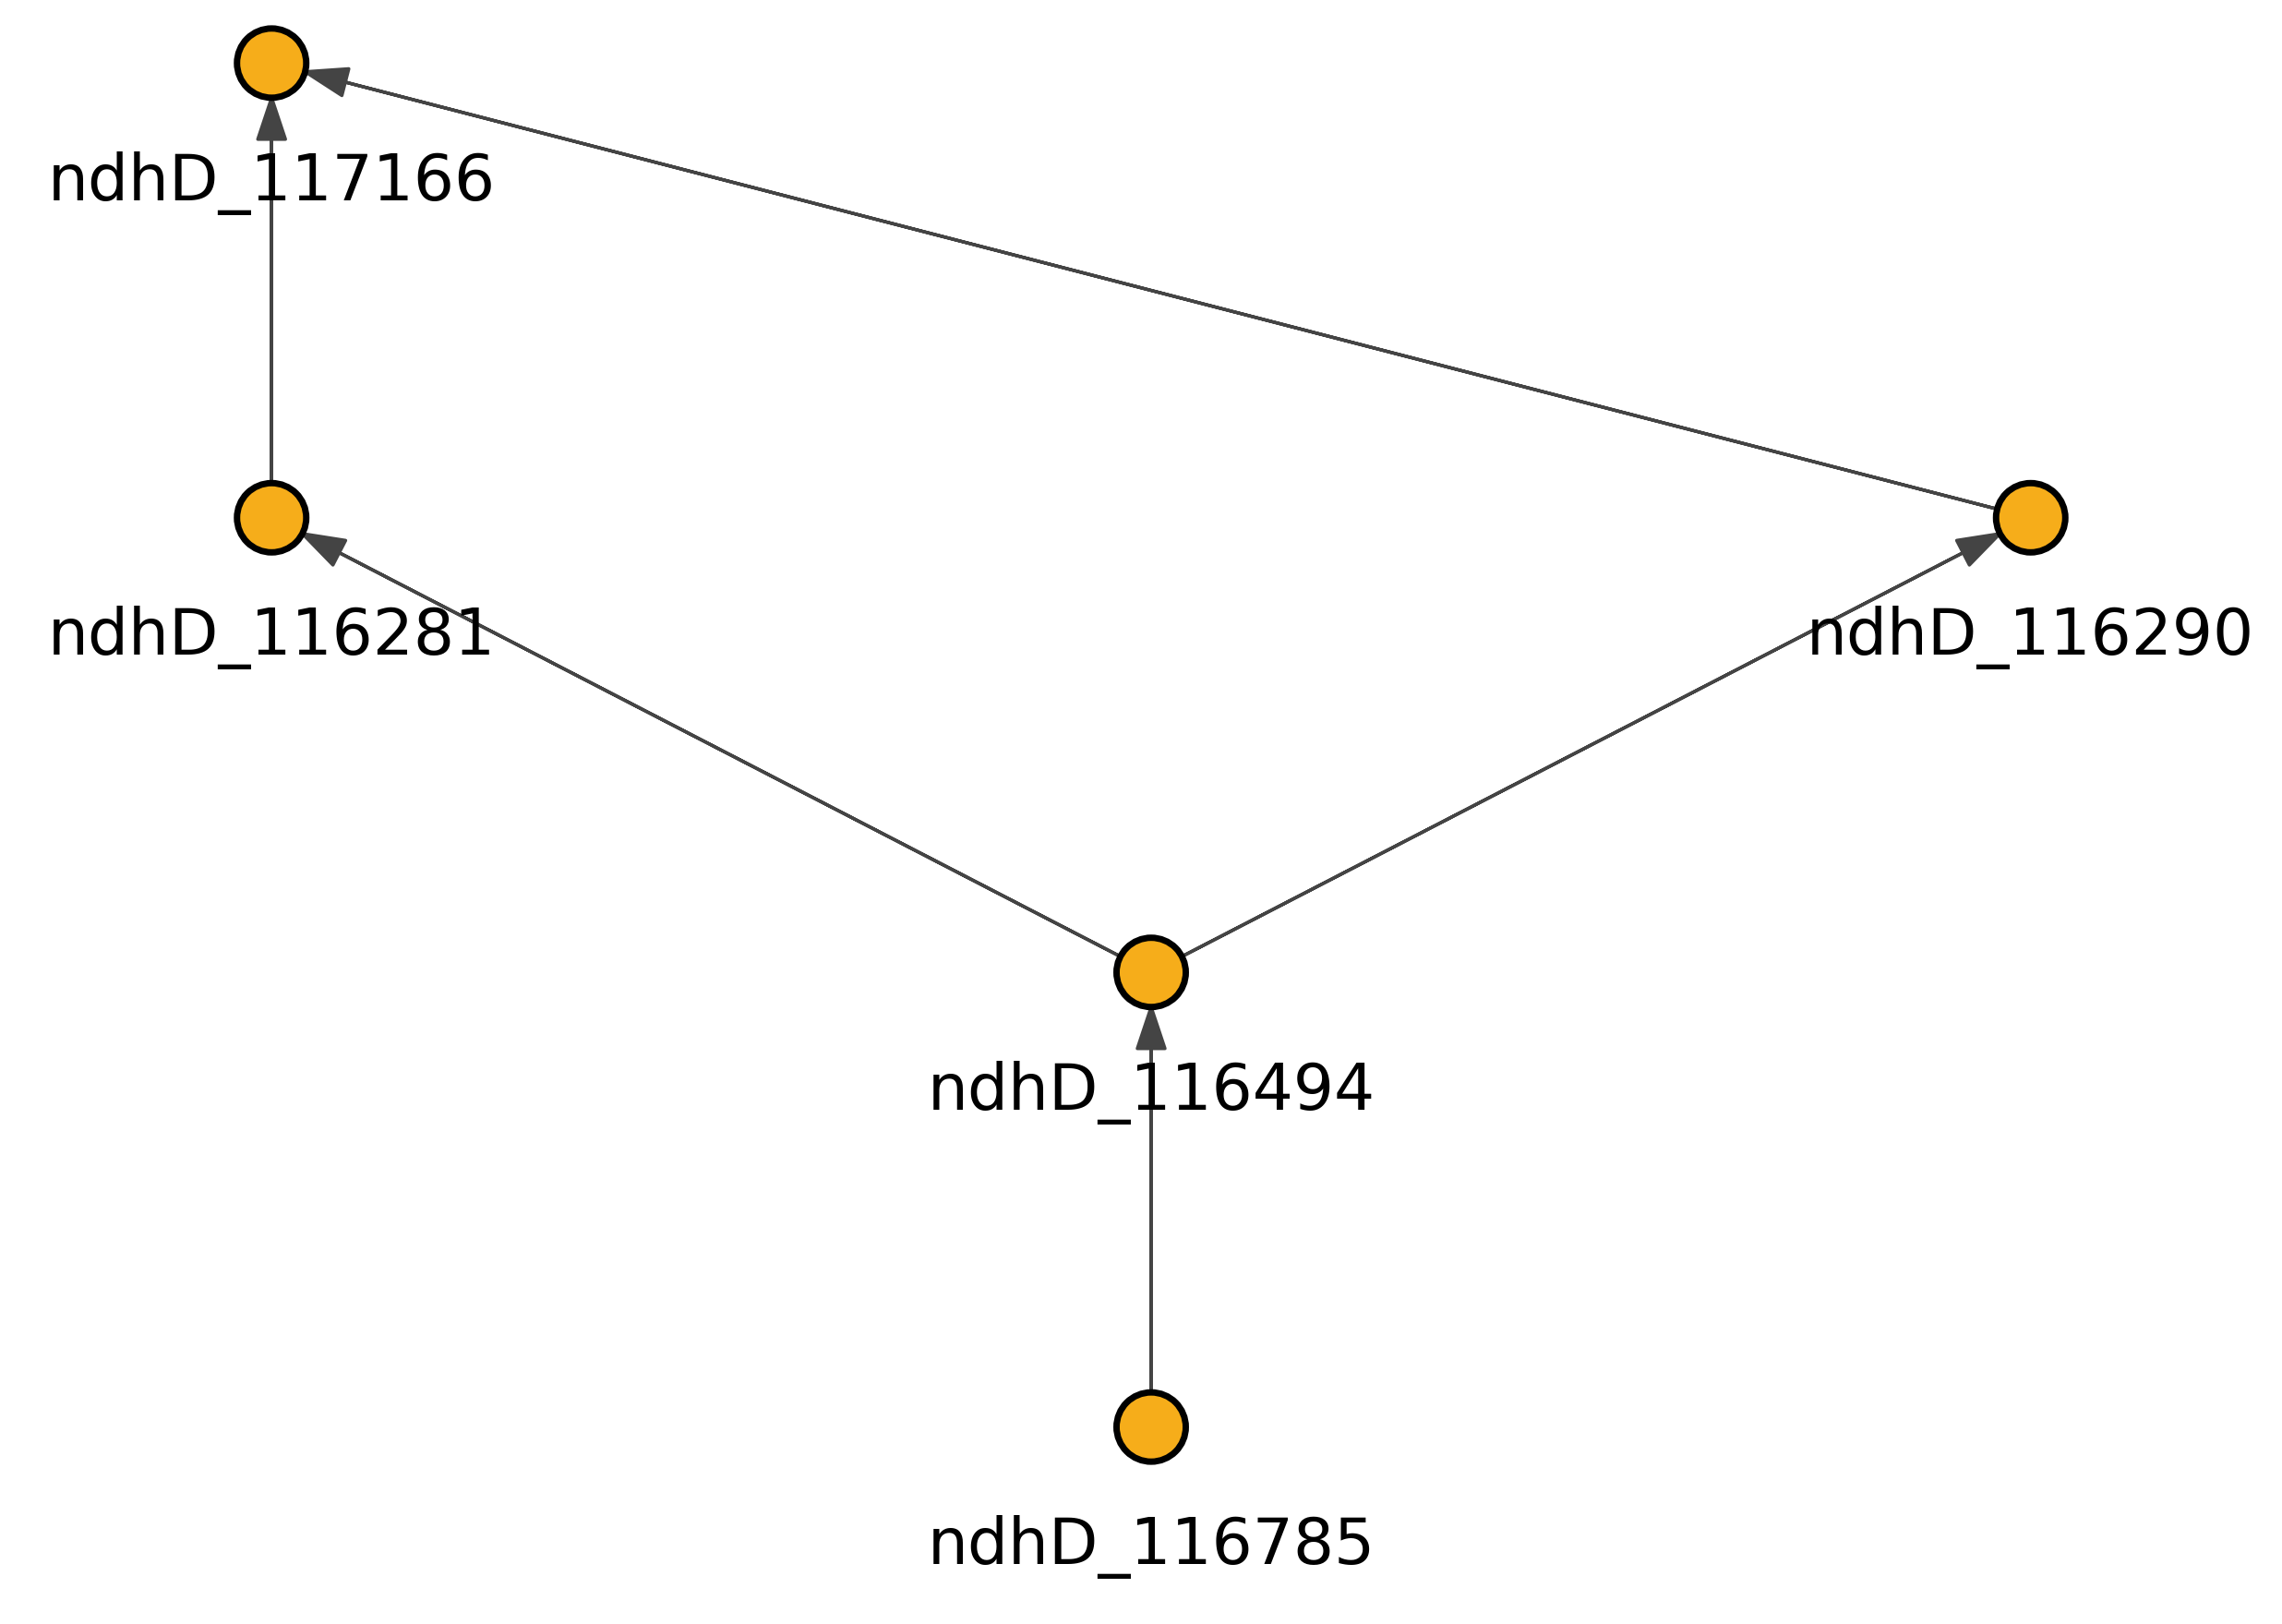
\includegraphics[width=3.125in,height=\textheight,keepaspectratio]{Figures Reference Graphs/chron_ndhD_Fig6.png}

\subcaption{\label{}\emph{ndhD}}
\end{minipage}%

\caption{\label{fig-ref_chrons}Reference models for maturation
chronology}

\end{figure}%

\begin{refremark}
Note that the reference timeline for \emph{ndhB}, illustrated in
Figure~\ref{fig-ref_chrons}, does not include the \emph{intron}. This is
because we observed that this event has an abnormally large effect on
the others. In fact, all graphs we recovered with the deterministic or
causal approach were unfalsifiable; removing this event makes them
falsifiable. We decided to remove from the analysis which is further
justified because, according to
\citeproc{ref-Long_Reads_GuilcherEtAl}{{[}1{]}}, the intron event
occurred at the very end of the timeline.

\label{rem-intron}

\end{refremark}

To conduct the comparison, we evaluated both sets of models
(causal-chronology vs.~reference) using two standard metrics: the
Bayesian Information Criterion (BIC) and the Log-Likelihood. The BIC
balances model fit with complexity, penalizing overfitting, while the
Log-Likelihood measures how well the model explains the observed data.

First, for each model we constructed a \texttt{DiscreteBayesianNetwork}
using the \texttt{pgmpy} library
(\citeproc{ref-pgmpyLibrary}{{[}27{]}}), and estimated its Conditional
Probability Distributions via a \texttt{BayesianEstimator}. We then
computed \texttt{structure\_score} (BIC) and
\texttt{log\_likelihood\_score} on both the reference and
causal-chronology networks. Implementation details and configuration
settings are available in our
\href{https://github.com/cambroise/chloroDAG}{GitHub repository}.

The results, compiled in the charts of Figure~\ref{fig-scores}, show
that at least one causal-chronology model dominates the reference model
in both BIC and log-likelihood. Importantly, \emph{ndhB} shows three
exceptions: the HC, PC and LiNGAM causal models underperform compared to
the reference. Note however that the PC model is close to the reference
model. Furthermore, performance differences are observed across causal
discovery algorithms. These exceptions and performance variations are
mainly due to the dataset size in terms of the number of variables. For
instance, NOTEARS achieved better scores than the other methods for
\emph{ndhB}, but not for \emph{ndhD}. Conversely, LiNGAM achieved better
scores than the other methods for \emph{ndhD}, but not for \emph{ndhB}.

\begin{figure}[H]

\begin{minipage}{0.43\linewidth}

\pandocbounded{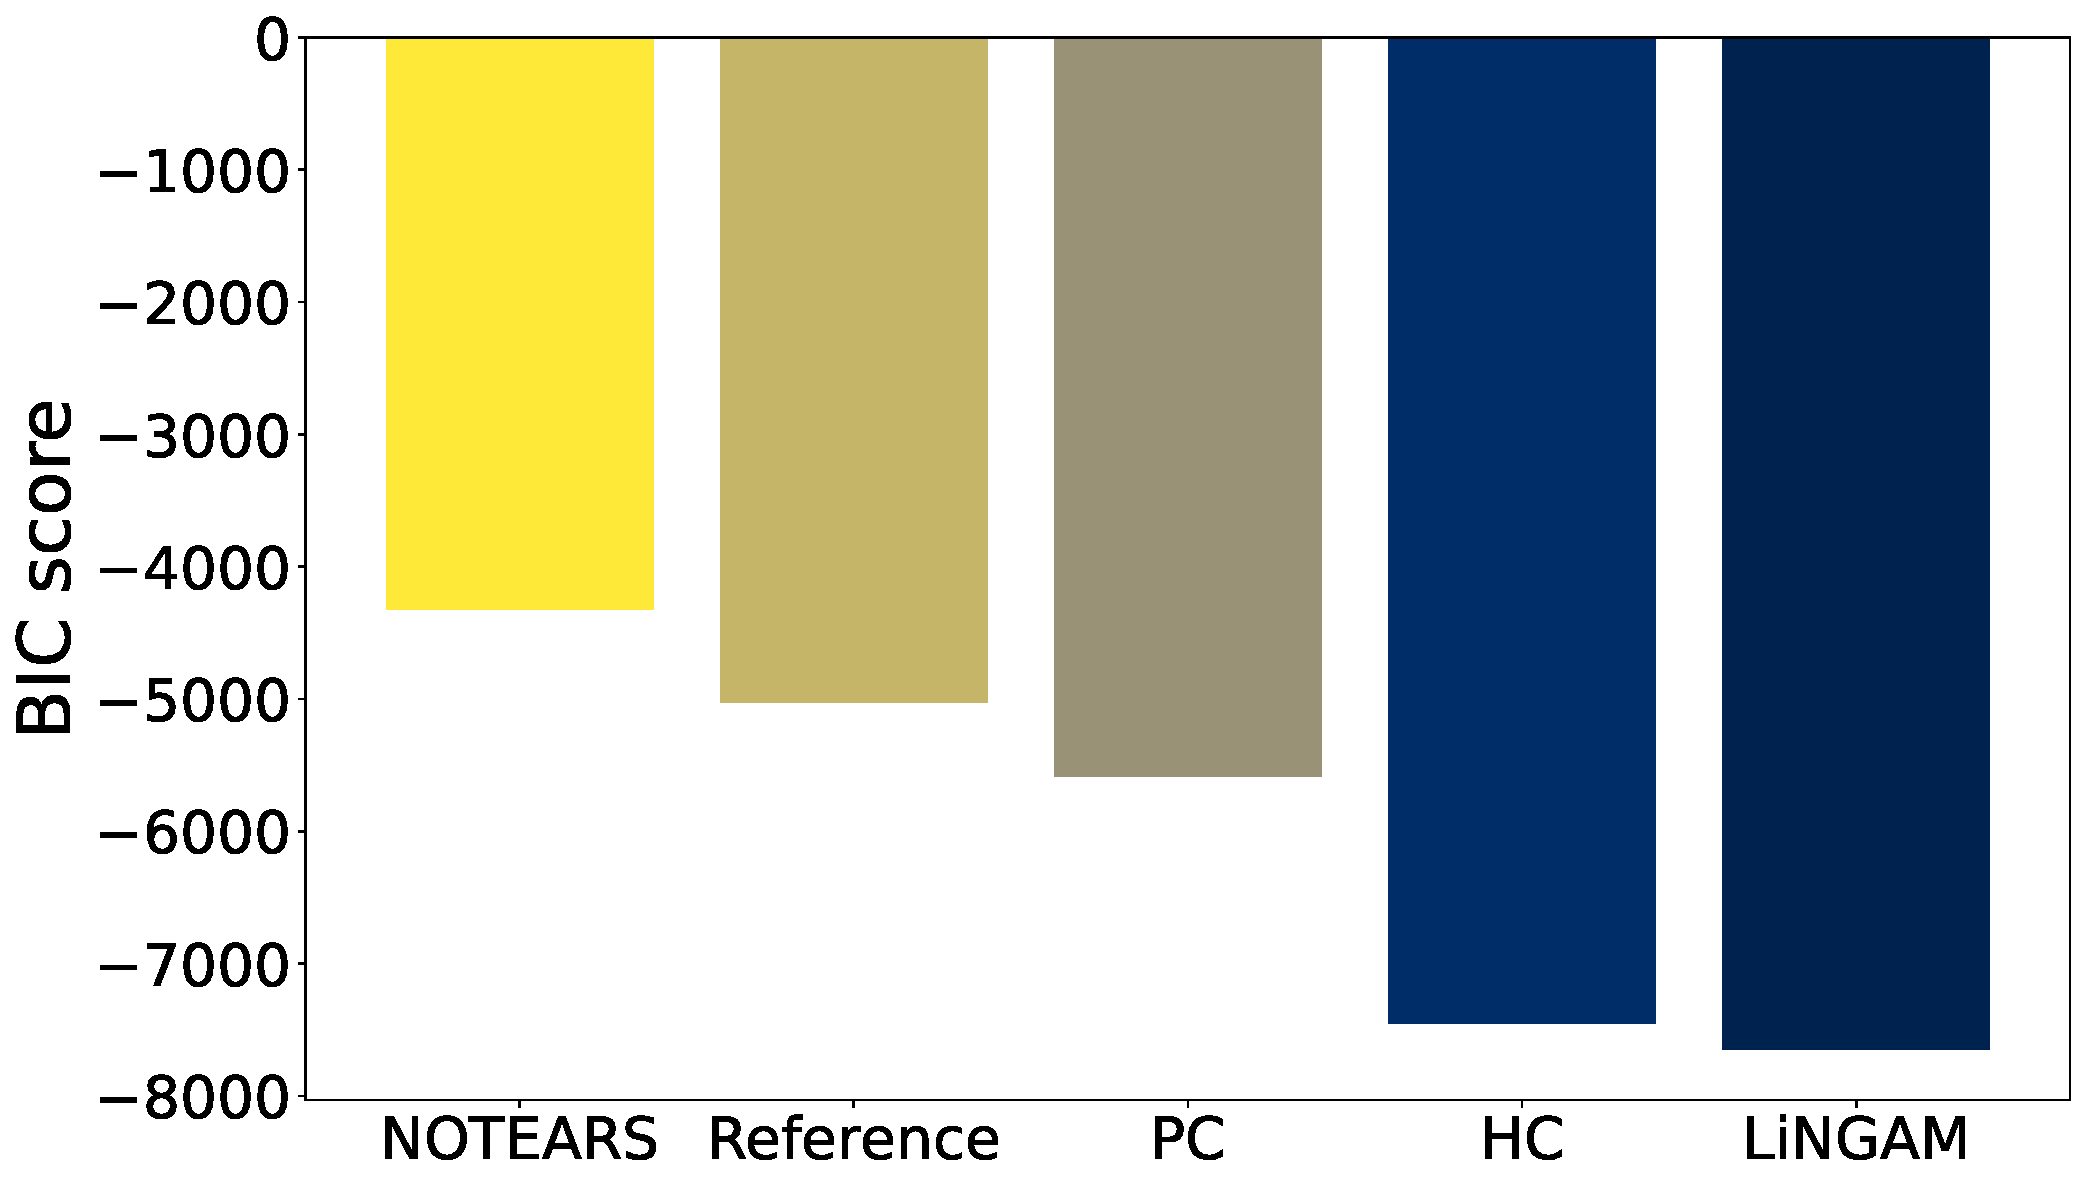
\includegraphics[keepaspectratio]{chloroDAG_files/figure-pdf/chart-bic_scores_ndhb-output-1.pdf}}

\subcaption{\label{}BIC scores for \emph{ndhB}}
\end{minipage}%
%
\begin{minipage}{0.13\linewidth}
~\end{minipage}%
%
\begin{minipage}{0.43\linewidth}

\pandocbounded{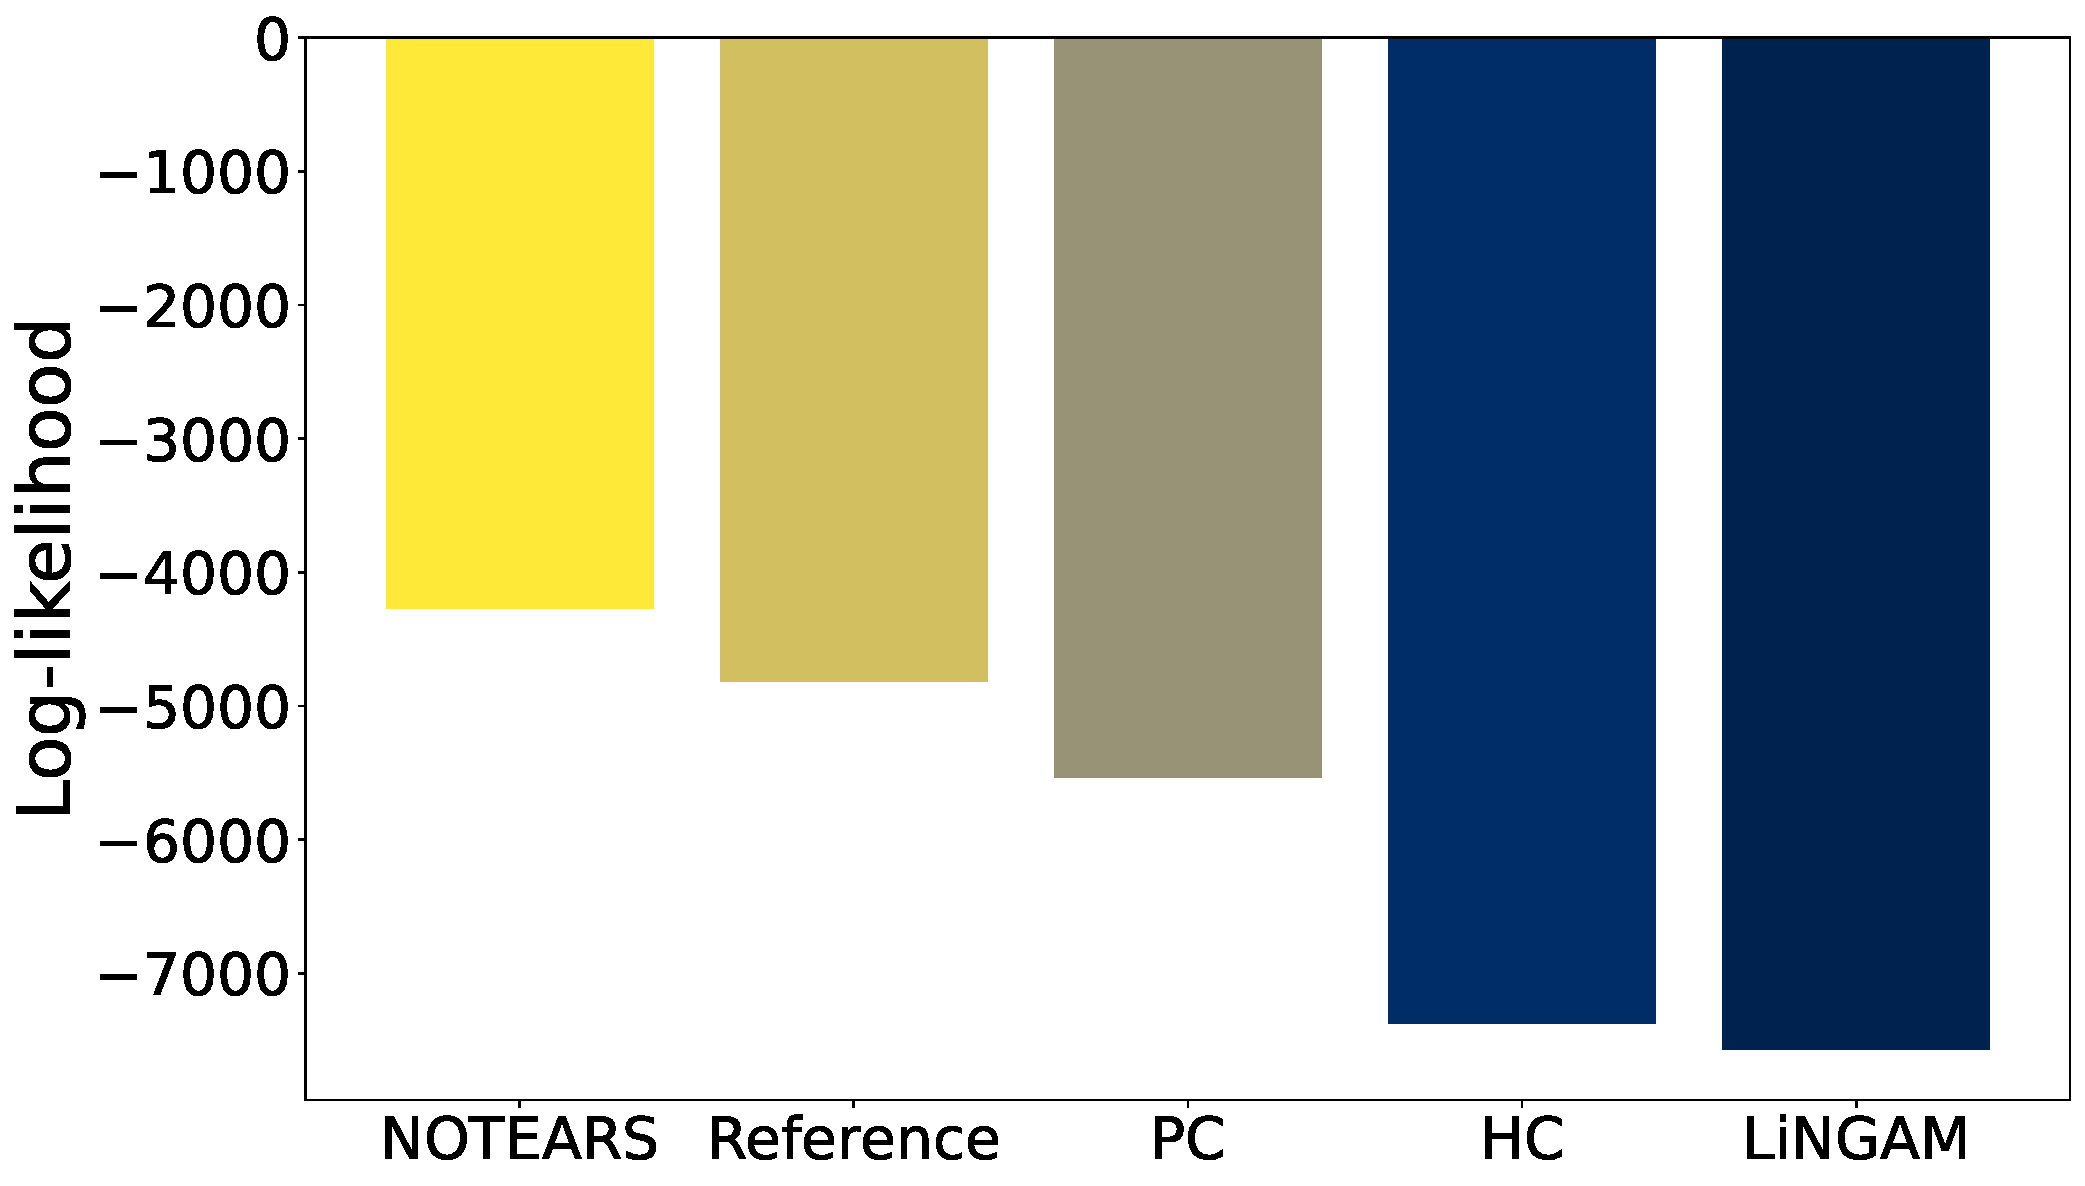
\includegraphics[keepaspectratio]{chloroDAG_files/figure-pdf/chart-logl_scores_ndhb-output-1.pdf}}

\subcaption{\label{}Log-likelihood scores for \emph{ndhB}}
\end{minipage}%
\newline
\begin{minipage}{0.43\linewidth}

\pandocbounded{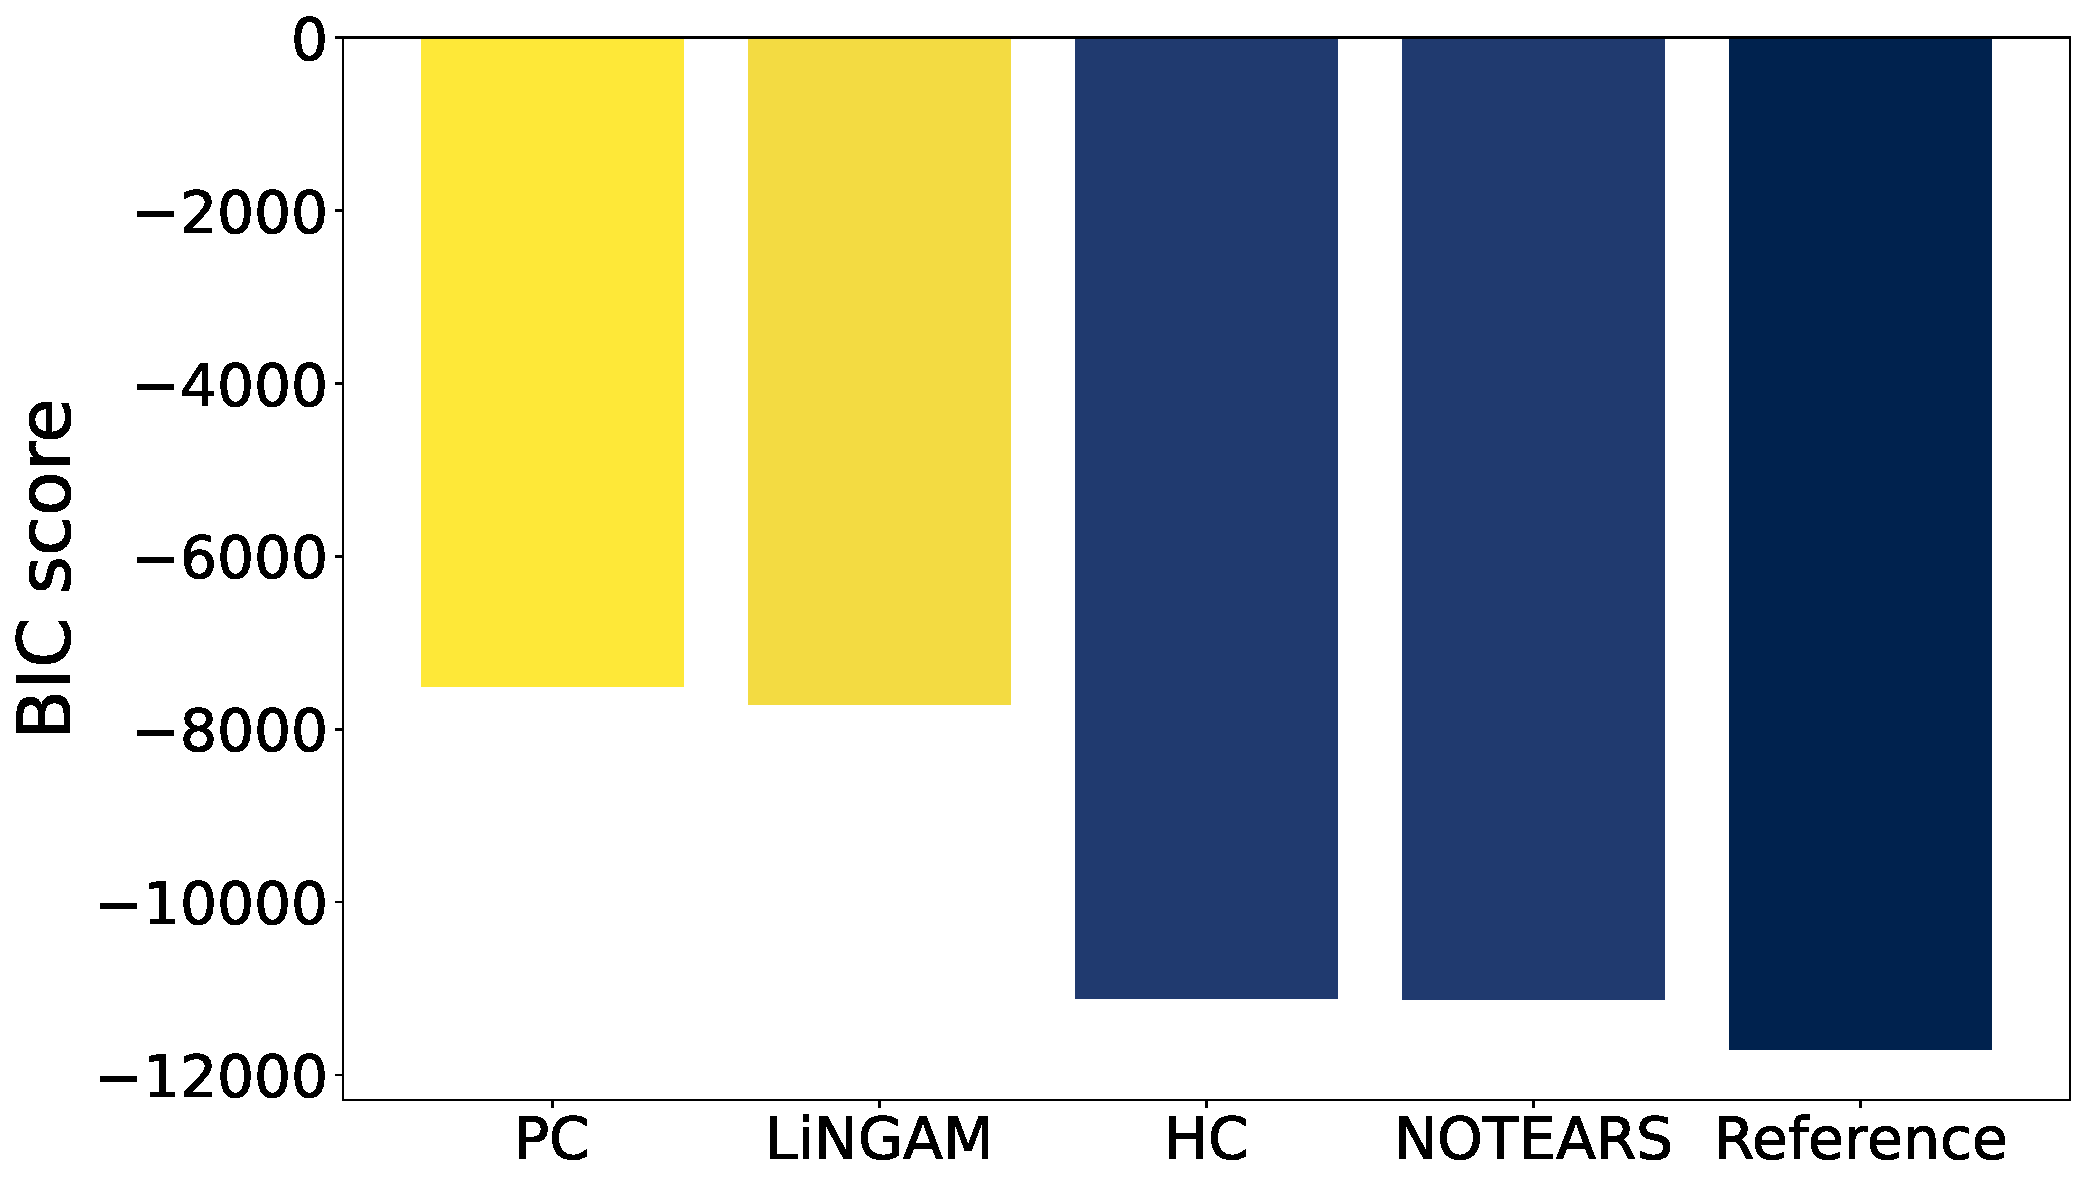
\includegraphics[keepaspectratio]{chloroDAG_files/figure-pdf/chart-bic_scores_ndhd-output-1.pdf}}

\subcaption{\label{}BIC scores for \emph{ndhD}}
\end{minipage}%
%
\begin{minipage}{0.13\linewidth}
~\end{minipage}%
%
\begin{minipage}{0.43\linewidth}

\pandocbounded{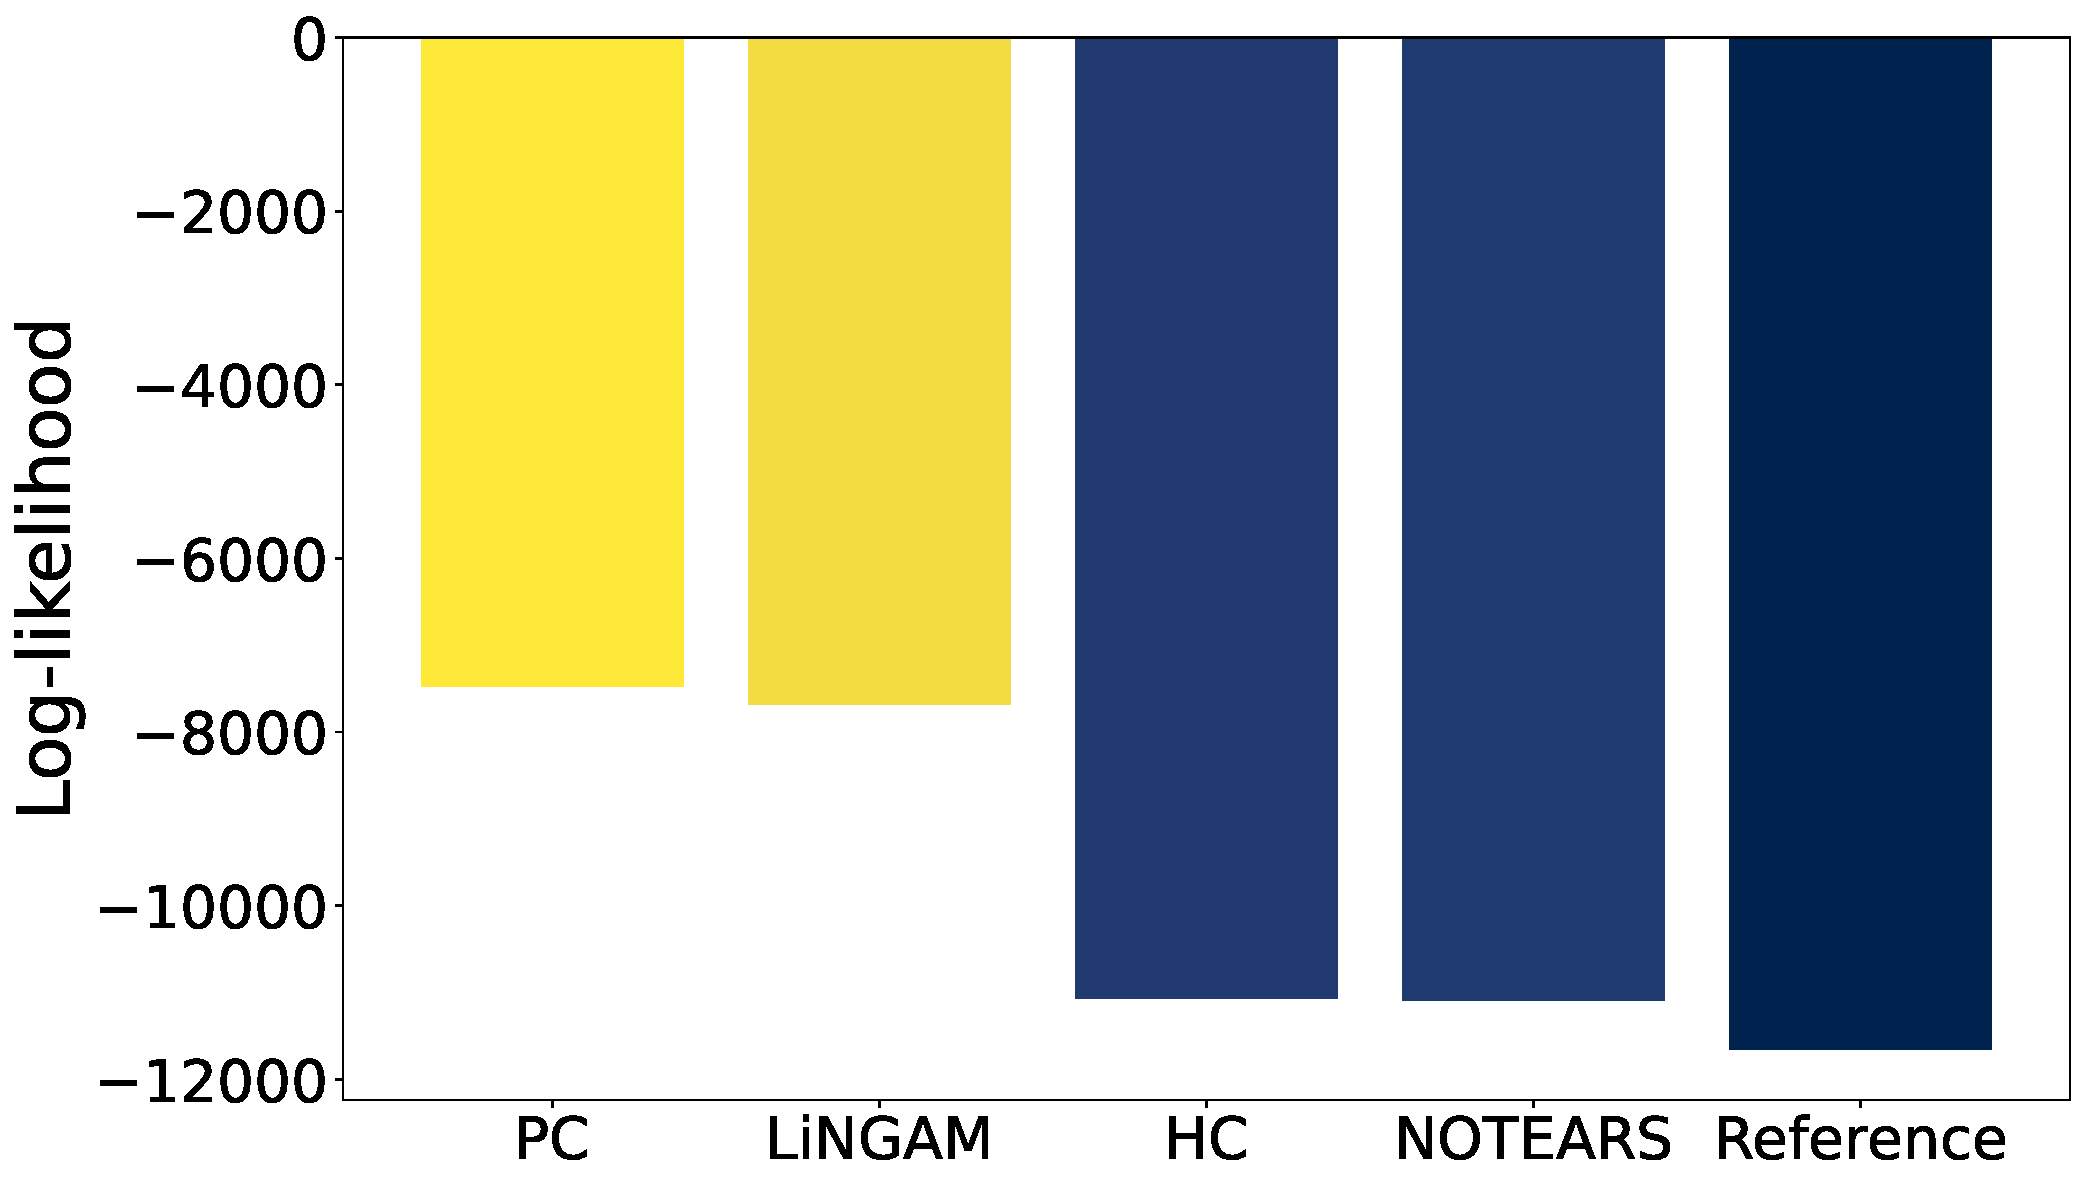
\includegraphics[keepaspectratio]{chloroDAG_files/figure-pdf/chart-logl_scores_ndhd-output-1.pdf}}

\subcaption{\label{}Log-likelihood scores for \emph{ndhD}}
\end{minipage}%

\caption{\label{fig-scores}Bar plots of standard metrics for
causal-chronology models and reference models: \emph{higher is better}.
Note that the scores (y-axes) are \emph{negative values}.}

\end{figure}%

A complementary metric used to compare our causal-chronology models to
the reference is based on the Bayesian network structure itself, as
explained in Section~\ref{sec-fals_tests}.
Figure~\ref{fig-falsification_summaries} summarizes the results of the
falsification tests conducted to assess whether the corresponding DAG is
accepted or rejected based on its fit with the provided data in terms of
conditional independencies. Notably, we observe in
Figure~\ref{fig-falsification_summaries} that there are always at least
two causal-chronology models that pass the tests with very high
performance. As for the reference model, it is rejected for \emph{ndhD}
and accepted for \emph{ndhB}.

\subsubsection{Reliability of the Proposed
Methodology}\label{sec-Reliability}

To conclude our case study, we assess the \textbf{reliability} of the
proposed methodology from two complementary perspectives: the stability
of the estimated causal effects and the validity of the inferred graph
structures.

\paragraph{Robustness of causal effect
estimates}\label{robustness-of-causal-effect-estimates}

The causal effects derived in our inference phase---such as the Average
Causal Effect (ACE), Natural Direct Effect (NDE), and Natural Indirect
Effect (NIE)---are influenced by modeling decisions, including the
structure of the underlying graph and the statistical estimators used.
To ensure that our results are not artifacts of specific configurations
or assumptions, we subject these estimates to robustness checks.

These include tests that examine whether effect estimates remain stable
under data perturbations, such as subsetting or introducing unrelated
variables. Additional checks evaluate whether the estimates degrade
appropriately when key assumptions are violated. Taken together, these
tests help identify estimates that are likely reliable versus those that
may be overly sensitive to modeling choices.

All reported causal effects (presented in Figure~\ref{fig-CR_ndhB} and
Figure~\ref{fig-CR_ndhD}) for which such analyses could be conducted
passed the relevant robustness checks. Full results are available at our
\href{https://github.com/cambroise/chloroDAG}{GitHub repository}.

\paragraph{Consistency of learned graph
structures}\label{sec-fals_tests}

Beyond individual effects, it is essential to validate the overall
graphical models produced during causal discovery. A well-specified DAG
should capture the key conditional independencies present in the data,
and differ meaningfully from random alternatives.

To this end, we assess whether each graph implies conditional
independence relations that are consistent with the observed data, and
whether the graph lies in a narrow equivalence class---indicating a
structure that is both specific and informative. These tests
collectively provide insight into whether the learned DAG captures more
than statistical noise or arbitrary correlations. The results
(summarized in Figure~\ref{fig-falsification_summaries}) reveal that
there are always at least two causal-chronology models that pass the
tests with very high performance.

\begin{figure}[H]

\begin{minipage}{0.43\linewidth}

\pandocbounded{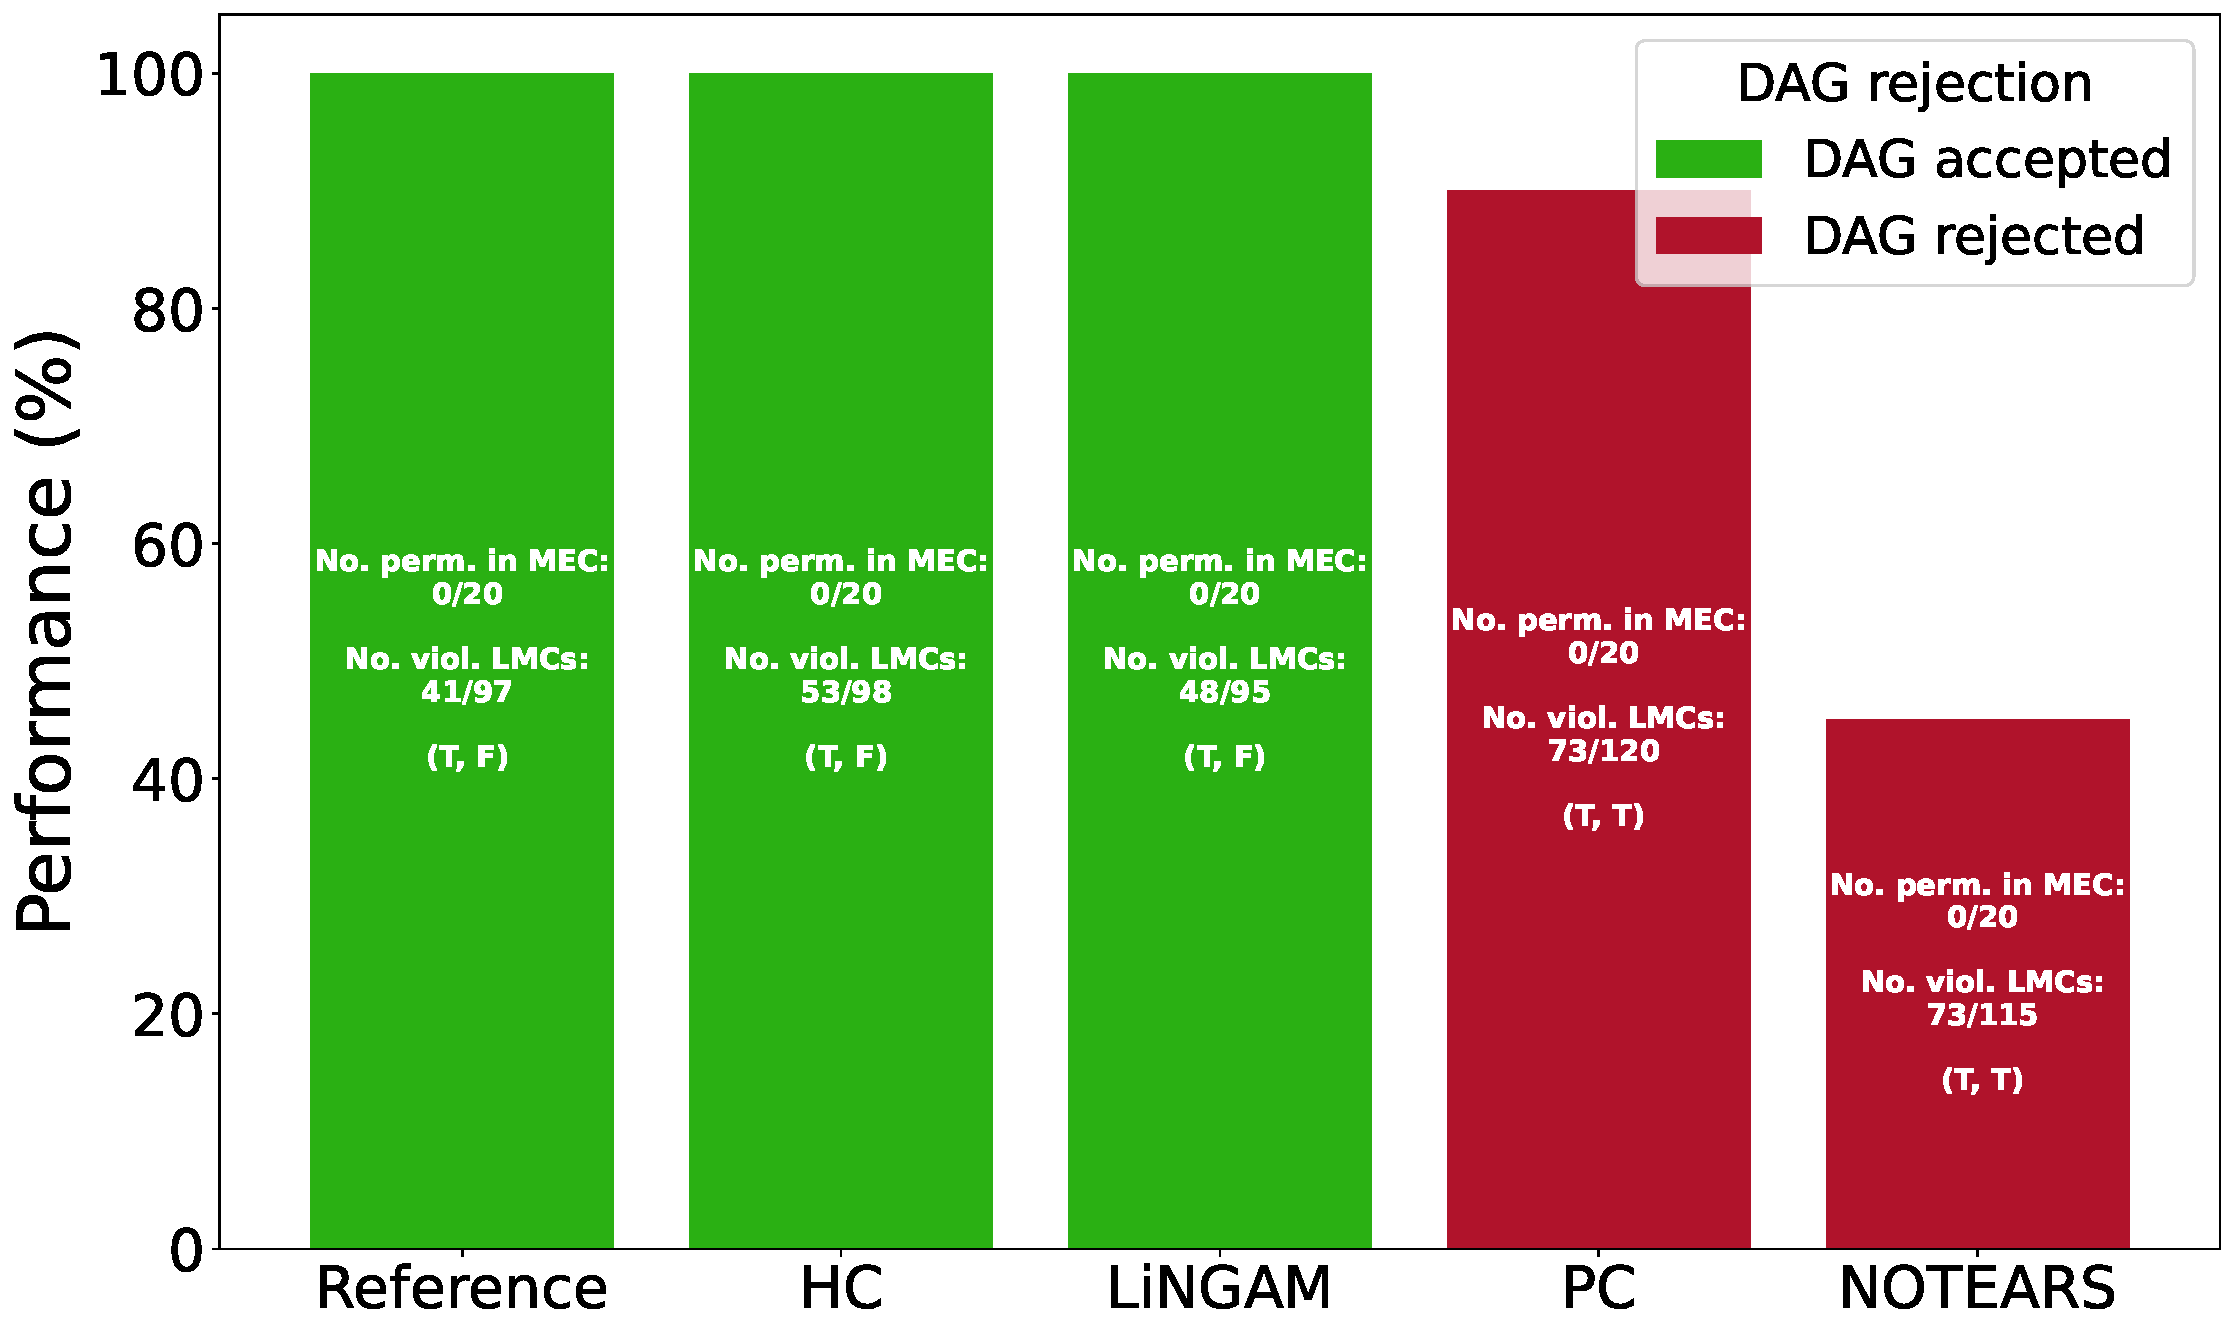
\includegraphics[keepaspectratio]{chloroDAG_files/figure-pdf/chart-falsificaton_ndhb-output-1.pdf}}

\subcaption{\label{}Falsification tests for \emph{ndhB}}
\end{minipage}%
%
\begin{minipage}{0.13\linewidth}
~\end{minipage}%
%
\begin{minipage}{0.43\linewidth}

\pandocbounded{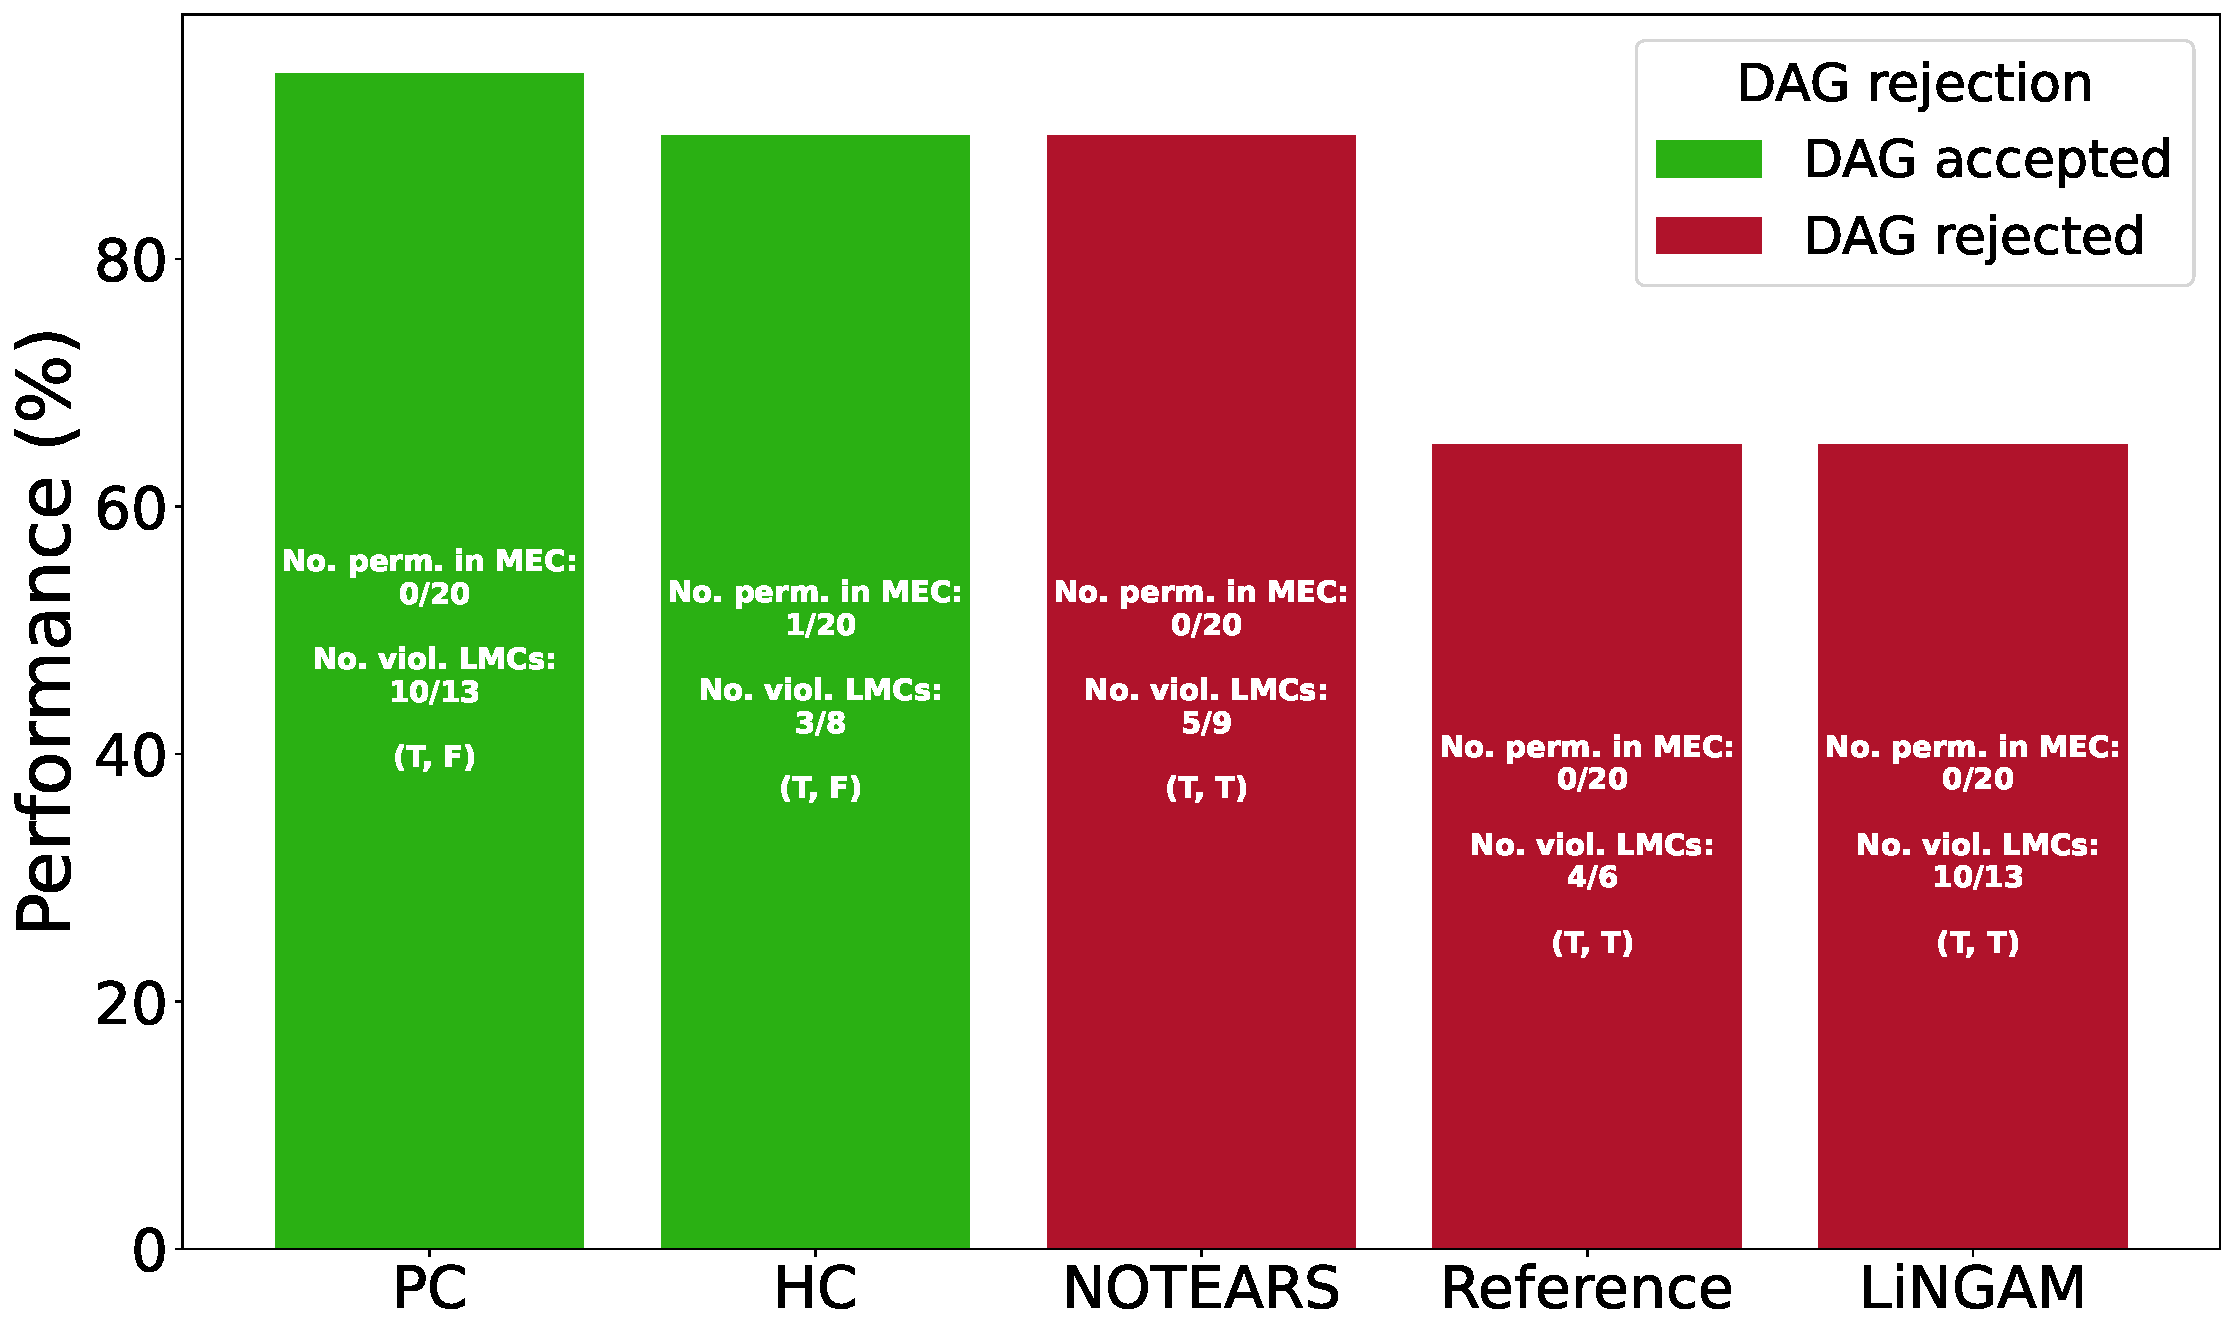
\includegraphics[keepaspectratio]{chloroDAG_files/figure-pdf/chart-falsificaton_ndhd-output-1.pdf}}

\subcaption{\label{}Falsification tests for \emph{ndhD}}
\end{minipage}%

\caption{\label{fig-falsification_summaries}Falsification summaries}

\end{figure}%

\begin{refremark}
Among the four possible (\emph{falsifiable}, \emph{falsified}) outcomes:

\begin{itemize}
\item
  (T, F): the DAG is likely valid or at least not contradicted by the
  data.
\item
  (T, T): the DAG is both specific and contradicted, therefore likely
  incorrect.
\item
  (F, F): inconclusive; the structure may be underdetermined by the
  data.
\item
  (F, T): an inconsistent outcome, suggesting possible issues with
  implementation or test assumptions.
\end{itemize}

It is worth noting that some causal structures---such as chains and
forks---are probabilistically indistinguishable. Therefore, even when
validation tests are passed, expert interpretation remains essential to
resolve ambiguities and confirm causal plausibility.

For all these reliability assessments, we leverage the tools available
in the \texttt{DoWhy} library.

\label{rem-falsification}

\end{refremark}

\section{Conclusive discussion}\label{sec-discussion}

We have introduced a new methodology for reconstructing the chronology
of genetic regulation events, grounded in Pearl's causal inference
framework. This probabilistic approach represents a conceptual shift
from earlier work in the field
\citeproc{ref-Long_Reads_GuilcherEtAl}{{[}1{]}}, moving beyond a
deterministic viewpoint modeling to explicit reasoning over
interventions. Our method captures the complex interplay of maturation
events---consistent with prior findings in the specialized literature
(e.g., \citeproc{ref-Heterologous_SchmitzEtAl}{{[}15{]}},
\citeproc{ref-LarchMito_MarechalEtAl}{{[}16{]}},
\citeproc{ref-ChloroCP31A_TillichEtAl}{{[}17{]}},
\citeproc{ref-SiteSelective_KarcherBock}{{[}18{]}},
\citeproc{ref-CisElements_TakenakaNeuwirtBrennicke}{{[}19{]}})---and
provides a well-founded strategy for extracting plausible maturation
timelines from transcriptomic datasets.

The methodology proceeds in three stages: 1. Causal discovery (learning
the DAG structure from data), 2. Causal inference (estimating the
effects of interventions), and 3. Chronology construction (building a
causal timeline as a tree-like graphical model).

We applied this pipeline to the post-transcriptional regulation of two
chloroplast genes, \emph{ndhB} and \emph{ndhD}, in \emph{Arabidopsis
thaliana}, generating four alternative causal-chronology models for each
gene. Each model corresponds to a distinct causal discovery algorithm.
Compared to the reference chronologies
\citeproc{ref-Long_Reads_GuilcherEtAl}{{[}1{]}}, our causal models
systematically achieved better fit for \emph{ndhD}, with NOTEARS
standing out for \emph{ndhB}, according to both the Bayesian Information
Criterion (BIC) and the log-likelihood. Furthermore, their robustness
was assessed through multiple refutation tests---both on individual
causal effect estimates and on the overall DAG structure---demonstrating
a consistent advantage over the reference models for \emph{ndhD}, while
the reference model remains valid for \emph{ndhB}.

We acknowledge that the causal discovery step introduces an element of
uncertainty, particularly in the presence of latent confounders or
limited data. As discussed in Remark~\ref{rem-falsification}, causal
structure learning cannot be fully validated from observational data
alone. To mitigate this limitation, we complemented standard approaches
(HC, PC, LiNGAM) with a continuous optimization-based method: NOTEARS
\citeproc{ref-DagsNotears}{{[}14{]}}. Because NOTEARS does not prescribe
a principled way to set the \(\ell_1\)-regularization parameter---which
governs the sparsity of the learned graph---we proposed a two-level
stability selection procedure. This approach was benchmarked using the
Sachs et al.~dataset and shown to improve structural reliability. While
\citeproc{ref-DagsNotears}{{[}14{]}} also reports results on this
dataset, it provides little insight into parameter tuning or
sensitivity.

A key practical challenge stemmed from the presence of numerous missing
values in the dataset. Naively restricting the analysis to fully
observed reads would have resulted in an unacceptable loss of
statistical power. Likewise, truncating the variable space to ensure
more complete rows would restrict biological interpretability and risk
introducing structural biases. To overcome this, we adopted a two-step
imputation strategy. First, we performed initial imputation using
IterativeImputer from scikit-learn. Then, a custom graphical model-based
EM algorithm iteratively refined the imputation and the DAG structure.
Interestingly, the choice of initial imputation method proved to have
minimal impact on the final graphical model.

Although our contribution is primarily computational, the proposed
framework naturally yields testable hypotheses and experimentally
verifiable predictions. The estimated causal effects are analogous to
those obtained in randomized controlled trials and can therefore inform
laboratory experiment design in a principled way. This opens the door to
more sophisticated causal analyses, including counterfactual reasoning
and targeted \emph{what if?} questions, thereby enriching the
interpretative power of long-read transcriptomic studies. These
perspectives are aligned with discussions held with the project leaders
of \citeproc{ref-Long_Reads_GuilcherEtAl}{{[}1{]}}.

In summary, we present a principled, flexible, and data-driven framework
for exploring gene regulation chronology. By combining causal discovery,
statistical inference, and domain expertise, it establishes a foundation
for reproducible, hypothesis-driven research in molecular biology.

\section*{References}\label{references}
\addcontentsline{toc}{section}{References}

\phantomsection\label{refs}
\begin{CSLReferences}{0}{0}
\bibitem[\citeproctext]{ref-Long_Reads_GuilcherEtAl}
\CSLLeftMargin{{[}1{]} }%
\CSLRightInline{M. Guilcher \emph{et al.}, {``Full length transcriptome
highlights the coordination of plastid transcript processing,''}
\emph{International Journal of Molecular Sciences}, vol. 22, no. 11297,
2021.}

\bibitem[\citeproctext]{ref-Margolin2006}
\CSLLeftMargin{{[}2{]} }%
\CSLRightInline{A. A. Margolin \emph{et al.}, {``ARACNE: An algorithm
for the reconstruction of gene regulatory networks in a mammalian
cellular context,''} \emph{BMC Bioinformatics}, vol. 7, no. Suppl 1, p.
S7, 2006, doi:
\href{https://doi.org/10.1186/1471-2105-7-S1-S7}{10.1186/1471-2105-7-S1-S7}.}

\bibitem[\citeproctext]{ref-Faith2007}
\CSLLeftMargin{{[}3{]} }%
\CSLRightInline{J. J. Faith \emph{et al.}, {``Large-scale mapping and
validation of *escherichia coli* transcriptional regulation from a
compendium of expression profiles,''} \emph{PLOS Biology}, vol. 5, no.
1, p. e8, 2007, doi:
\href{https://doi.org/10.1371/journal.pbio.0050008}{10.1371/journal.pbio.0050008}.}

\bibitem[\citeproctext]{ref-Meyer2008_minet}
\CSLLeftMargin{{[}4{]} }%
\CSLRightInline{P. E. Meyer, F. Lafitte, and G. Bontempi, {``Minet: An
r/bioconductor package for inferring large transcriptional networks
using mutual information,''} \emph{BMC Bioinformatics}, vol. 9, p. 461,
2008, doi:
\href{https://doi.org/10.1186/1471-2105-9-461}{10.1186/1471-2105-9-461}.}

\bibitem[\citeproctext]{ref-HuynhThu2010}
\CSLLeftMargin{{[}5{]} }%
\CSLRightInline{V. A. Huynh-Thu, A. Irrthum, L. Wehenkel, and P. Geurts,
{``Inferring regulatory networks from expression data using tree-based
methods,''} \emph{PLOS ONE}, vol. 5, no. 9, p. e12776, 2010, doi:
\href{https://doi.org/10.1371/journal.pone.0012776}{10.1371/journal.pone.0012776}.}

\bibitem[\citeproctext]{ref-Friedman2000}
\CSLLeftMargin{{[}6{]} }%
\CSLRightInline{N. Friedman, M. Linial, I. Nachman, and D. Peer,
{``Using bayesian networks to analyze expression data,''} \emph{Journal
of Computational Biology}, vol. 7, no. 3--4, pp. 601--620, 2000, doi:
\href{https://doi.org/10.1089/106652700750050961}{10.1089/106652700750050961}.}

\bibitem[\citeproctext]{ref-Pearl2009}
\CSLLeftMargin{{[}7{]} }%
\CSLRightInline{J. Pearl, \emph{Causality: Models, reasoning and
inference}, 2nd ed. Cambridge University Press, 2009. Available:
\url{https://projects.illc.uva.nl/cil/uploaded_files/inlineitem/Pearl_2009_Causality.pdf}}

\bibitem[\citeproctext]{ref-HuynhThuGeurts2018}
\CSLLeftMargin{{[}8{]} }%
\CSLRightInline{V. A. Huynh-Thu and P. Geurts, {``dynGENIE3: Dynamical
{GENIE3} for the inference of gene networks from time series expression
data,''} \emph{Scientific Reports}, vol. 8, no. 1, p. 3384, 2018, doi:
\href{https://doi.org/10.1038/s41598-018-21715-0}{10.1038/s41598-018-21715-0}.}

\bibitem[\citeproctext]{ref-Murphy2002DBN}
\CSLLeftMargin{{[}9{]} }%
\CSLRightInline{K. P. Murphy, {``Dynamic bayesian networks:
Representation, inference and learning,''} PhD thesis, University of
California, Berkeley, 2002. Available:
\url{https://www2.eecs.berkeley.edu/Pubs/TechRpts/2002/8174.html}}

\bibitem[\citeproctext]{ref-PapiliGao2018SINCERITIES}
\CSLLeftMargin{{[}10{]} }%
\CSLRightInline{N. Papili Gao, S. M. Ud-Dean, O. Gandrillon, and R.
Gunawan, {``SINCERITIES: Inferring gene regulatory networks from
time-stamped single cell transcriptional expression profiles,''}
\emph{Bioinformatics}, vol. 34, no. 2, pp. 258--266, 2018, doi:
\href{https://doi.org/10.1093/bioinformatics/btx622}{10.1093/bioinformatics/btx622}.}

\bibitem[\citeproctext]{ref-Moerman2019GRNBoost2}
\CSLLeftMargin{{[}11{]} }%
\CSLRightInline{T. Moerman \emph{et al.}, {``Efficient and scalable
inference of gene regulatory networks,''} \emph{Bioinformatics}, vol.
35, no. 12, pp. 2159--2161, 2019, doi:
\href{https://doi.org/10.1093/bioinformatics/bty916}{10.1093/bioinformatics/bty916}.}

\bibitem[\citeproctext]{ref-Guilcher2025}
\CSLLeftMargin{{[}12{]} }%
\CSLRightInline{J. Guilcher, L. Lezhneva, R. Williams-Carrier, A.
Barkan, I. Small, and K. Hammani, {``Full length transcriptome
highlights the coordination of plastid transcript processing,''}
\emph{The Plant Cell}, 2025, Available:
\url{https://hal.inrae.fr/hal-03343771}}

\bibitem[\citeproctext]{ref-CausalityBook_Pearl}
\CSLLeftMargin{{[}13{]} }%
\CSLRightInline{J. Pearl, \emph{Causality: Models, reasoning, and
inference}, Second edition. 32 Avenue of the Americas, New York, NY,
USA: Cambridge University Press, 2009.}

\bibitem[\citeproctext]{ref-DagsNotears}
\CSLLeftMargin{{[}14{]} }%
\CSLRightInline{X. Zheng, B. Aragam, P. Ravikumar, and E. P. Xing,
{``DAGs with NO TEARS: Continuous optimization for structure
learning,''} in \emph{Proceedings of the 32nd international conference
on neural information processing systems}, in NIPS'18. Red Hook, NY,
USA: Curran Associates Inc., 2018, pp. 9492--9503.}

\bibitem[\citeproctext]{ref-Heterologous_SchmitzEtAl}
\CSLLeftMargin{{[}15{]} }%
\CSLRightInline{C. Schmitz‐Linneweber, M. Tillich, R. G. Herrmann, and
R. M. Maier, {``Heterologous, splicing-dependent RNA editing in
chloroplasts: Allotetraploidy provides trans-factors,''} \emph{The EMBO
Journal}, vol. 20, no. 17, pp. 4874--4883, 2001.}

\bibitem[\citeproctext]{ref-LarchMito_MarechalEtAl}
\CSLLeftMargin{{[}16{]} }%
\CSLRightInline{L. Maréchal-Drouard, R. Kumar, C. Remacle, and I. Small,
{``RNA editing of larch mitochondrial tRNA his precursors is a
prerequisite for processing,''} \emph{Nucleic Acids Research}, vol. 24,
no. 16, pp. 3229--3234, 1996.}

\bibitem[\citeproctext]{ref-ChloroCP31A_TillichEtAl}
\CSLLeftMargin{{[}17{]} }%
\CSLRightInline{M. Tillich \emph{et al.}, {``Chloroplast
ribonucleoprotein CP31A is required for editing and stability of
specific chloroplast mRNAs,''} \emph{Proceedings of the National Academy
of Sciences}, vol. 106, no. 14, pp. 6002--6007, 2009.}

\bibitem[\citeproctext]{ref-SiteSelective_KarcherBock}
\CSLLeftMargin{{[}18{]} }%
\CSLRightInline{D. Karcher and R. Bock, {``Site-selective inhibition of
plastid RNA editing by heat shock and antibiotics: A role for plastid
translation in RNA editing,''} \emph{Nucleic Acids Research}, vol. 26,
no. 5, pp. 1185--1190, 1998.}

\bibitem[\citeproctext]{ref-CisElements_TakenakaNeuwirtBrennicke}
\CSLLeftMargin{{[}19{]} }%
\CSLRightInline{M. Takenaka, J. Neuwirt, and A. Brennicke, {``Complex
cis-elements determine an RNA editing site in pea mitochondria,''}
\emph{Nucleic Acids Research}, vol. 32, no. 14, pp. 4137--4144, 2004.}

\bibitem[\citeproctext]{ref-TeyssierKoller2005}
\CSLLeftMargin{{[}20{]} }%
\CSLRightInline{M. Teyssier and D. Koller, {``Ordering‑based search: A
simple and effective algorithm for learning bayesian networks,''} in
\emph{Proceedings of the 21st conference on uncertainty in artificial
intelligence (UAI)}, 2005, pp. 584--590.}

\bibitem[\citeproctext]{ref-CausalityPaper_Pearl}
\CSLLeftMargin{{[}21{]} }%
\CSLRightInline{J. Pearl, {``Causal diagrams for empirical research,''}
\emph{Biometrika}, vol. 82, no. 4, pp. 669--688, 1995.}

\bibitem[\citeproctext]{ref-spirtes1993causation}
\CSLLeftMargin{{[}22{]} }%
\CSLRightInline{P. Spirtes, C. Glymour, and R. Scheines,
\emph{Causation, prediction, and search}. New York: Springer-Verlag,
1993.}

\bibitem[\citeproctext]{ref-shimizu2006linear}
\CSLLeftMargin{{[}23{]} }%
\CSLRightInline{S. Shimizu, P. O. Hoyer, A. Hyvärinen, and A. Kerminen,
{``A linear non-gaussian acyclic model for causal discovery,''}
\emph{Journal of Machine Learning Research}, vol. 7, pp. 2003--2030,
2006.}

\bibitem[\citeproctext]{ref-scikit-learnLibrary}
\CSLLeftMargin{{[}24{]} }%
\CSLRightInline{F. Pedregosa \emph{et al.}, {``Scikit-learn: Machine
learning in {P}ython,''} \emph{Journal of Machine Learning Research},
vol. 12, pp. 2825--2830, 2011.}

\bibitem[\citeproctext]{ref-IntelligentSystemsBook_Pearl}
\CSLLeftMargin{{[}25{]} }%
\CSLRightInline{J. Pearl, \emph{Probabilistic reasoning in intelligent
systems: Networks of plausible inference}. Morgan Kaufmann Publishers
Inc., 1988.}

\bibitem[\citeproctext]{ref-LoopyBP}
\CSLLeftMargin{{[}26{]} }%
\CSLRightInline{K. P. Murphy, Y. Weiss, and M. I. Jordan, {``Loopy
belief propagation for approximate inference: An empirical study,''} in
\emph{Proceedings of the fifteenth conference on uncertainty in
artificial intelligence}, in UAI'99, no. 9. San Francisco, CA, USA:
Morgan Kaufmann Publishers Inc., 1999, pp. 467--475.}

\bibitem[\citeproctext]{ref-pgmpyLibrary}
\CSLLeftMargin{{[}27{]} }%
\CSLRightInline{A. Ankan and J. Textor, {``Pgmpy: A python toolkit for
bayesian networks,''} \emph{Journal of Machine Learning Research}, vol.
25, no. 265, pp. 1--8, 2024.}

\bibitem[\citeproctext]{ref-CausalLearnLibrary}
\CSLLeftMargin{{[}28{]} }%
\CSLRightInline{Y. Zheng \emph{et al.}, {``Causal-learn: Causal
discovery in python,''} \emph{Journal of Machine Learning Research},
vol. 25, no. 60, pp. 1--8, 2024.}

\bibitem[\citeproctext]{ref-dowhy}
\CSLLeftMargin{{[}29{]} }%
\CSLRightInline{P. Blöbaum, P. Götz, K. Budhathoki, A. A. Mastakouri,
and D. Janzing, {``DoWhy‑GCM: An extension of DoWhy for causal inference
in graphical causal models,''} \emph{Journal of Machine Learning
Research}, vol. 25, no. 147, pp. 1--7, 2024, Available:
\url{http://jmlr.org/papers/v25/22-1258.html}}

\bibitem[\citeproctext]{ref-igraphLibrary}
\CSLLeftMargin{{[}30{]} }%
\CSLRightInline{G. Csardi and T. Nepusz, {``The igraph software package
for complex network research,''} \emph{InterJournal, Complex Systems},
no. 1695, 2006.}

\bibitem[\citeproctext]{ref-KaiserSipos2021}
\CSLLeftMargin{{[}31{]} }%
\CSLRightInline{M. Kaiser and M. Sipos, {``{Unsuitability of NOTEARS for
Causal Graph Discovery},''} \emph{arXiv preprint arXiv:2104.05441},
2021, Available: \url{https://arxiv.org/abs/2104.05441}}

\end{CSLReferences}

\newpage{}

\section{Appendices}\label{appendices}

\subsection{NOTEARS as a causal discovery algorithm}\label{sec-notears}

We adapted the NOTEARS algorithm \citeproc{ref-DagsNotears}{{[}14{]}} as
part of our causal discovery pipeline. NOTEARS formulates the search for
a DAG structure as a continuous optimization problem over a weighted
adjacency matrix \(W\), avoiding the combinatorial complexity of
traditional structure learning. The acyclicity constraint is enforced
using a smooth algebraic function, and sparsity is promoted via
\(\ell_1\) regularization. The result is a differentiable objective that
can be optimized using gradient-based methods.

In our setting, we observed that NOTEARS was highly sensitive to the
choice of the regularization parameter \(\lambda\), with small changes
leading to radically different graph structures. To address this, we
introduced a two-level stability selection strategy (full details are
available at our \href{https://github.com/cambroise/chloroDAG}{GitHub
repository}):

\begin{enumerate}
\def\labelenumi{\arabic{enumi}.}
\tightlist
\item
  For a grid of \(\lambda\) values, we performed multiple resampling
  iterations (bootstrap or sub-sampling) of the input data.
\item
  For each configuration, we recorded the set of directed edges returned
  by NOTEARS.
\item
  We defined a directed edge as \emph{stable} if it appeared frequently
  across both resamplings and a contiguous range of regularization
  parameters, avoiding overly sparse or overly dense configurations.
\end{enumerate}

This approach allowed us to construct a robust DAG by retaining only
stable directed edges. It mitigates two known limitations of NOTEARS:
its sensitivity to hyperparameters and the lack of invariance to
variable rescaling \citeproc{ref-KaiserSipos2021}{{[}31{]}}.

While the resulting graphs were more interpretable and robust, it is
worth noting that NOTEARS relies on a linear SEM assumption, and its
optimization is non-convex. Therefore, learned graphs should be
interpreted as hypotheses supported by data, rather than definitive
causal claims. As such, we cross-validated NOTEARS outputs with those of
HC, PC, and LiNGAM, and report only consistently supported edges in the
final causal timelines.

\subsection{Causal inference
results}\label{sec-causal_inference_results}

\begin{figure}[H]

\begin{minipage}{0.43\linewidth}

\pandocbounded{\includegraphics[keepaspectratio]{chloroDAG_files/figure-pdf/chart-causality_hc_ndhb-output-1.pdf}}

\subcaption{\label{}Causal effects for the HC-model}
\end{minipage}%
%
\begin{minipage}{0.13\linewidth}
~\end{minipage}%
%
\begin{minipage}{0.43\linewidth}

\pandocbounded{\includegraphics[keepaspectratio]{chloroDAG_files/figure-pdf/chart-causality_pc_ndhb-output-1.pdf}}

\subcaption{\label{}Causal effects for the PC-model}
\end{minipage}%
\newline
\begin{minipage}{0.43\linewidth}

\pandocbounded{\includegraphics[keepaspectratio]{chloroDAG_files/figure-pdf/chart-causality_lingam_ndhb-output-1.pdf}}

\subcaption{\label{}Causal effects for the LiNGAM-model}
\end{minipage}%
%
\begin{minipage}{0.13\linewidth}
~\end{minipage}%
%
\begin{minipage}{0.43\linewidth}

\pandocbounded{\includegraphics[keepaspectratio]{chloroDAG_files/figure-pdf/chart-causality_notears_ndhb-output-1.pdf}}

\subcaption{\label{}Causal effects for the NOTEARS-model}
\end{minipage}%

\caption{\label{fig-CR_ndhB}Causal relations for \emph{ndhB}}

\end{figure}%

\begin{figure}[H]

\begin{minipage}{0.43\linewidth}

\pandocbounded{\includegraphics[keepaspectratio]{chloroDAG_files/figure-pdf/chart-causality_hc_ndhd-output-1.pdf}}

\subcaption{\label{}Causal effects for the HC-model}
\end{minipage}%
%
\begin{minipage}{0.13\linewidth}
~\end{minipage}%
%
\begin{minipage}{0.43\linewidth}

\pandocbounded{\includegraphics[keepaspectratio]{chloroDAG_files/figure-pdf/chart-causality_pc_ndhd-output-1.pdf}}

\subcaption{\label{}Causal effects for the PC-model}
\end{minipage}%
\newline
\begin{minipage}{0.43\linewidth}

\pandocbounded{\includegraphics[keepaspectratio]{chloroDAG_files/figure-pdf/chart-causality_lingam_ndhd-output-1.pdf}}

\subcaption{\label{}Causal effects for the LiNGAM-model}
\end{minipage}%
%
\begin{minipage}{0.13\linewidth}
~\end{minipage}%
%
\begin{minipage}{0.43\linewidth}

\pandocbounded{\includegraphics[keepaspectratio]{chloroDAG_files/figure-pdf/chart-causality_notears_ndhd-output-1.pdf}}

\subcaption{\label{}Causal effects for the NOTEARS-model}
\end{minipage}%

\caption{\label{fig-CR_ndhD}Causal relations for \emph{ndhD}}

\end{figure}%




\end{document}
